\documentclass[twoside]{book}

% Packages required by doxygen
\usepackage{fixltx2e}
\usepackage{calc}
\usepackage{doxygen}
\usepackage[export]{adjustbox} % also loads graphicx
\usepackage{graphicx}
\usepackage[utf8]{inputenc}
\usepackage{makeidx}
\usepackage{multicol}
\usepackage{multirow}
\PassOptionsToPackage{warn}{textcomp}
\usepackage{textcomp}
\usepackage[nointegrals]{wasysym}
\usepackage[table]{xcolor}

% NLS support packages
\usepackage[brazil]{babel}
% Font selection
\usepackage[T1]{fontenc}
\usepackage[scaled=.90]{helvet}
\usepackage{courier}
\usepackage{amssymb}
\usepackage{sectsty}
\renewcommand{\familydefault}{\sfdefault}
\allsectionsfont{%
  \fontseries{bc}\selectfont%
  \color{darkgray}%
}
\renewcommand{\DoxyLabelFont}{%
  \fontseries{bc}\selectfont%
  \color{darkgray}%
}
\newcommand{\+}{\discretionary{\mbox{\scriptsize$\hookleftarrow$}}{}{}}

% Page & text layout
\usepackage{geometry}
\geometry{%
  a4paper,%
  top=2.5cm,%
  bottom=2.5cm,%
  left=2.5cm,%
  right=2.5cm%
}
\tolerance=750
\hfuzz=15pt
\hbadness=750
\setlength{\emergencystretch}{15pt}
\setlength{\parindent}{0cm}
\setlength{\parskip}{0.2cm}
\makeatletter
\renewcommand{\paragraph}{%
  \@startsection{paragraph}{4}{0ex}{-1.0ex}{1.0ex}{%
    \normalfont\normalsize\bfseries\SS@parafont%
  }%
}
\renewcommand{\subparagraph}{%
  \@startsection{subparagraph}{5}{0ex}{-1.0ex}{1.0ex}{%
    \normalfont\normalsize\bfseries\SS@subparafont%
  }%
}
\makeatother

% Headers & footers
\usepackage{fancyhdr}
\pagestyle{fancyplain}
\fancyhead[LE]{\fancyplain{}{\bfseries\thepage}}
\fancyhead[CE]{\fancyplain{}{}}
\fancyhead[RE]{\fancyplain{}{\bfseries\leftmark}}
\fancyhead[LO]{\fancyplain{}{\bfseries\rightmark}}
\fancyhead[CO]{\fancyplain{}{}}
\fancyhead[RO]{\fancyplain{}{\bfseries\thepage}}
\fancyfoot[LE]{\fancyplain{}{}}
\fancyfoot[CE]{\fancyplain{}{}}
\fancyfoot[RE]{\fancyplain{}{\bfseries\scriptsize Gerado por Doxygen }}
\fancyfoot[LO]{\fancyplain{}{\bfseries\scriptsize Gerado por Doxygen }}
\fancyfoot[CO]{\fancyplain{}{}}
\fancyfoot[RO]{\fancyplain{}{}}
\renewcommand{\footrulewidth}{0.4pt}
\renewcommand{\chaptermark}[1]{%
  \markboth{#1}{}%
}
\renewcommand{\sectionmark}[1]{%
  \markright{\thesection\ #1}%
}

% Indices & bibliography
\usepackage{natbib}
\usepackage[titles]{tocloft}
\setcounter{tocdepth}{3}
\setcounter{secnumdepth}{5}
\makeindex

% Hyperlinks (required, but should be loaded last)
\usepackage{ifpdf}
\ifpdf
  \usepackage[pdftex,pagebackref=true]{hyperref}
\else
  \usepackage[ps2pdf,pagebackref=true]{hyperref}
\fi
\hypersetup{%
  colorlinks=true,%
  linkcolor=blue,%
  citecolor=blue,%
  unicode%
}

% Custom commands
\newcommand{\clearemptydoublepage}{%
  \newpage{\pagestyle{empty}\cleardoublepage}%
}


%===== C O N T E N T S =====

\begin{document}

% Titlepage & ToC
\hypersetup{pageanchor=false,
             bookmarks=true,
             bookmarksnumbered=true,
             pdfencoding=unicode
            }
\pagenumbering{roman}
\begin{titlepage}
\vspace*{7cm}
\begin{center}%
{\Large Trabalho de Grafos \\[1ex]\large 1 }\\
\vspace*{1cm}
{\large Gerado por Doxygen 1.8.10}\\
\end{center}
\end{titlepage}
\clearemptydoublepage
\tableofcontents
\clearemptydoublepage
\pagenumbering{arabic}
\hypersetup{pageanchor=true}

%--- Begin generated contents ---
\chapter{Índice das Estruturas de Dados}
\section{Estruturas de Dados}
Aqui estão as estruturas de dados, uniões e suas respectivas descrições\+:\begin{DoxyCompactList}
\item\contentsline{section}{\hyperlink{structCelula__priv}{Celula\+\_\+priv} }{\pageref{structCelula__priv}}{}
\item\contentsline{section}{\hyperlink{structgrafo__priv}{grafo\+\_\+priv} }{\pageref{structgrafo__priv}}{}
\item\contentsline{section}{\hyperlink{structlista__aresta}{lista\+\_\+aresta} }{\pageref{structlista__aresta}}{}
\item\contentsline{section}{\hyperlink{structlista__origem}{lista\+\_\+origem} }{\pageref{structlista__origem}}{}
\item\contentsline{section}{\hyperlink{structlista__vert}{lista\+\_\+vert} }{\pageref{structlista__vert}}{}
\item\contentsline{section}{\hyperlink{structlista__vert__codigo}{lista\+\_\+vert\+\_\+codigo} }{\pageref{structlista__vert__codigo}}{}
\item\contentsline{section}{\hyperlink{structModulo}{Modulo} }{\pageref{structModulo}}{}
\end{DoxyCompactList}

\chapter{Índice dos Arquivos}
\section{Lista de Arquivos}
Esta é a lista de todos os arquivos e suas respectivas descrições\+:\begin{DoxyCompactList}
\item\contentsline{section}{/home/rafael/\+Projeto\+Final\+M\+P/\+Fase2\+Interface/include/\hyperlink{grafo_8h}{grafo.\+h} \\*Define funções usadas pelo usuario }{\pageref{grafo_8h}}{}
\item\contentsline{section}{/home/rafael/\+Projeto\+Final\+M\+P/\+Fase2\+Interface/include/\hyperlink{grafo__priv_8h}{grafo\+\_\+priv.\+h} }{\pageref{grafo__priv_8h}}{}
\item\contentsline{section}{\hyperlink{grafo_8cpp}{grafo.\+cpp} }{\pageref{grafo_8cpp}}{}
\item\contentsline{section}{\hyperlink{interface_8cpp}{interface.\+cpp} }{\pageref{interface_8cpp}}{}
\end{DoxyCompactList}

\chapter{Estruturas}
\hypertarget{structCelula__priv}{}\section{Referência da Estrutura Celula\+\_\+priv}
\label{structCelula__priv}\index{Celula\+\_\+priv@{Celula\+\_\+priv}}


{\ttfamily \#include $<$grafo\+\_\+priv.\+h$>$}

\subsection*{Campos de Dados}
\begin{DoxyCompactItemize}
\item 
int \hyperlink{structCelula__priv_a78a8525da28e1918d0faaf127001bd7b}{id\+\_\+externo}
\item 
int \hyperlink{structCelula__priv_af5f995caad41372e844f965021c5d183}{executada}
\item 
int \hyperlink{structCelula__priv_aee72d429cf8e17c945a1eb4e05ad85c7}{duracao}
\item 
int \hyperlink{structCelula__priv_a3c49601fe078bd7bb1512f0107af5301}{ini\+\_\+min}
\item 
int \hyperlink{structCelula__priv_a3ff8d3c4d0ba994771391320203619fc}{pre\+\_\+req}
\item 
int $\ast$ \hyperlink{structCelula__priv_ad54839cd4d96e78a58c226ab2e8d0579}{reqs}
\item 
char \hyperlink{structCelula__priv_a7f33fa72aceed7b44922f0f39d6f7f59}{nome} \mbox{[}200\mbox{]}
\end{DoxyCompactItemize}


\subsection{Descrição Detalhada}


Definição na linha 6 do arquivo grafo\+\_\+priv.\+h.



\subsection{Campos}
\hypertarget{structCelula__priv_aee72d429cf8e17c945a1eb4e05ad85c7}{}\index{Celula\+\_\+priv@{Celula\+\_\+priv}!duracao@{duracao}}
\index{duracao@{duracao}!Celula\+\_\+priv@{Celula\+\_\+priv}}
\subsubsection[{duracao}]{\setlength{\rightskip}{0pt plus 5cm}int Celula\+\_\+priv\+::duracao}\label{structCelula__priv_aee72d429cf8e17c945a1eb4e05ad85c7}


Definição na linha 7 do arquivo grafo\+\_\+priv.\+h.



Referenciado por cria\+\_\+celula(), cria\+Grafo\+Arq(), editar\+\_\+celula(), Grava\+\_\+\+Arq(), Imprime\+\_\+\+Tarefas(), interface\+\_\+inserir\+\_\+tarefa() e interface\+\_\+vizualizar\+\_\+determinada\+\_\+tarefa().

\hypertarget{structCelula__priv_af5f995caad41372e844f965021c5d183}{}\index{Celula\+\_\+priv@{Celula\+\_\+priv}!executada@{executada}}
\index{executada@{executada}!Celula\+\_\+priv@{Celula\+\_\+priv}}
\subsubsection[{executada}]{\setlength{\rightskip}{0pt plus 5cm}int Celula\+\_\+priv\+::executada}\label{structCelula__priv_af5f995caad41372e844f965021c5d183}


Definição na linha 7 do arquivo grafo\+\_\+priv.\+h.



Referenciado por cria\+\_\+celula(), cria\+Grafo\+Arq(), criar\+\_\+grafo(), editar\+\_\+celula(), Grava\+\_\+\+Arq(), Imprime\+\_\+\+Tarefas(), interface\+\_\+inserir\+\_\+tarefa() e interface\+\_\+vizualizar\+\_\+determinada\+\_\+tarefa().

\hypertarget{structCelula__priv_a78a8525da28e1918d0faaf127001bd7b}{}\index{Celula\+\_\+priv@{Celula\+\_\+priv}!id\+\_\+externo@{id\+\_\+externo}}
\index{id\+\_\+externo@{id\+\_\+externo}!Celula\+\_\+priv@{Celula\+\_\+priv}}
\subsubsection[{id\+\_\+externo}]{\setlength{\rightskip}{0pt plus 5cm}int Celula\+\_\+priv\+::id\+\_\+externo}\label{structCelula__priv_a78a8525da28e1918d0faaf127001bd7b}


Definição na linha 7 do arquivo grafo\+\_\+priv.\+h.



Referenciado por achar\+\_\+celula(), achar\+\_\+id(), cria\+\_\+celula(), cria\+Grafo\+Arq(), criar\+\_\+grafo(), deletar\+\_\+grafo(), editar\+\_\+celula(), existe\+\_\+vert(), Grava\+\_\+\+Arq(), Imprime\+\_\+\+Tarefas(), inserir\+\_\+aresta(), inserir\+\_\+origem(), inserir\+\_\+vert(), interface\+\_\+inserir\+\_\+tarefa() e interface\+\_\+vizualizar\+\_\+determinada\+\_\+tarefa().

\hypertarget{structCelula__priv_a3c49601fe078bd7bb1512f0107af5301}{}\index{Celula\+\_\+priv@{Celula\+\_\+priv}!ini\+\_\+min@{ini\+\_\+min}}
\index{ini\+\_\+min@{ini\+\_\+min}!Celula\+\_\+priv@{Celula\+\_\+priv}}
\subsubsection[{ini\+\_\+min}]{\setlength{\rightskip}{0pt plus 5cm}int Celula\+\_\+priv\+::ini\+\_\+min}\label{structCelula__priv_a3c49601fe078bd7bb1512f0107af5301}


Definição na linha 8 do arquivo grafo\+\_\+priv.\+h.



Referenciado por cria\+\_\+celula(), cria\+Grafo\+Arq(), criar\+\_\+grafo(), editar\+\_\+celula(), Grava\+\_\+\+Arq(), Imprime\+\_\+\+Tarefas(), inserir\+\_\+vert(), interface\+\_\+inserir\+\_\+tarefa(), interface\+\_\+vizualizar\+\_\+determinada\+\_\+tarefa() e menor\+\_\+caminho().

\hypertarget{structCelula__priv_a7f33fa72aceed7b44922f0f39d6f7f59}{}\index{Celula\+\_\+priv@{Celula\+\_\+priv}!nome@{nome}}
\index{nome@{nome}!Celula\+\_\+priv@{Celula\+\_\+priv}}
\subsubsection[{nome}]{\setlength{\rightskip}{0pt plus 5cm}char Celula\+\_\+priv\+::nome\mbox{[}200\mbox{]}}\label{structCelula__priv_a7f33fa72aceed7b44922f0f39d6f7f59}


Definição na linha 10 do arquivo grafo\+\_\+priv.\+h.



Referenciado por cria\+\_\+celula(), cria\+Grafo\+Arq(), criar\+\_\+grafo(), editar\+\_\+celula(), Grava\+\_\+\+Arq(), Imprime\+\_\+\+Tarefas(), inserir\+\_\+aresta(), inserir\+\_\+origem(), inserir\+\_\+vert(), interface\+\_\+inserir\+\_\+tarefa() e interface\+\_\+vizualizar\+\_\+determinada\+\_\+tarefa().

\hypertarget{structCelula__priv_a3ff8d3c4d0ba994771391320203619fc}{}\index{Celula\+\_\+priv@{Celula\+\_\+priv}!pre\+\_\+req@{pre\+\_\+req}}
\index{pre\+\_\+req@{pre\+\_\+req}!Celula\+\_\+priv@{Celula\+\_\+priv}}
\subsubsection[{pre\+\_\+req}]{\setlength{\rightskip}{0pt plus 5cm}int Celula\+\_\+priv\+::pre\+\_\+req}\label{structCelula__priv_a3ff8d3c4d0ba994771391320203619fc}


Definição na linha 8 do arquivo grafo\+\_\+priv.\+h.



Referenciado por cria\+\_\+celula(), cria\+Grafo\+Arq(), criar\+\_\+grafo(), editar\+\_\+celula(), Grava\+\_\+\+Arq(), Imprime\+\_\+\+Tarefas(), inserir\+\_\+vert(), interface\+\_\+inserir\+\_\+tarefa() e interface\+\_\+vizualizar\+\_\+determinada\+\_\+tarefa().

\hypertarget{structCelula__priv_ad54839cd4d96e78a58c226ab2e8d0579}{}\index{Celula\+\_\+priv@{Celula\+\_\+priv}!reqs@{reqs}}
\index{reqs@{reqs}!Celula\+\_\+priv@{Celula\+\_\+priv}}
\subsubsection[{reqs}]{\setlength{\rightskip}{0pt plus 5cm}int$\ast$ Celula\+\_\+priv\+::reqs}\label{structCelula__priv_ad54839cd4d96e78a58c226ab2e8d0579}


Definição na linha 9 do arquivo grafo\+\_\+priv.\+h.



Referenciado por cria\+\_\+celula(), cria\+Grafo\+Arq(), editar\+\_\+celula(), Grava\+\_\+\+Arq(), Imprime\+\_\+\+Tarefas(), interface\+\_\+inserir\+\_\+tarefa() e interface\+\_\+vizualizar\+\_\+determinada\+\_\+tarefa().



A documentação para esta estrutura foi gerada a partir do seguinte arquivo\+:\begin{DoxyCompactItemize}
\item 
/home/rafael/\+Projeto\+Final\+M\+P/\+Fase2\+Interface/include/\hyperlink{grafo__priv_8h}{grafo\+\_\+priv.\+h}\end{DoxyCompactItemize}

\hypertarget{structgrafo__priv}{}\section{Referência da Estrutura grafo\+\_\+priv}
\label{structgrafo__priv}\index{grafo\+\_\+priv@{grafo\+\_\+priv}}


{\ttfamily \#include $<$grafo\+\_\+priv.\+h$>$}



Diagrama de colaboração para grafo\+\_\+priv\+:\nopagebreak
\begin{figure}[H]
\begin{center}
\leavevmode
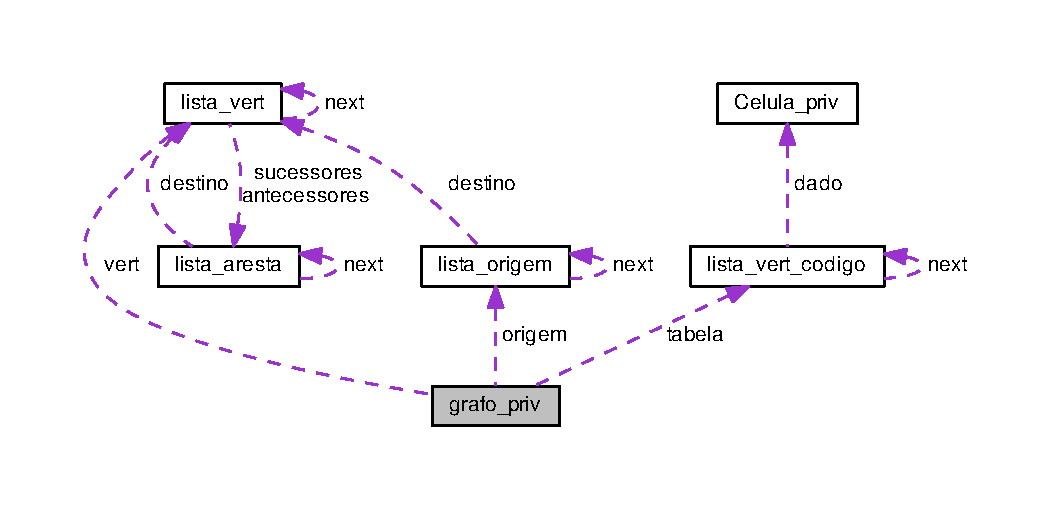
\includegraphics[width=350pt]{structgrafo__priv__coll__graph}
\end{center}
\end{figure}
\subsection*{Campos de Dados}
\begin{DoxyCompactItemize}
\item 
\hyperlink{grafo__priv_8h_ae17c76eddcd8bd44e7d91faf7c00e2e5}{lista\+\_\+vert\+\_\+codigo\+\_\+t} $\ast$ \hyperlink{structgrafo__priv_a7aaee4699517501a8ca504043ef78ddb}{tabela}
\item 
\hyperlink{grafo__priv_8h_aecb68281fecb412bf6427dd6a07d5077}{lista\+\_\+vert\+\_\+t} $\ast$ \hyperlink{structgrafo__priv_a6f7e609364c2e69e02c56860b1a2c3ad}{vert}
\item 
\hyperlink{grafo__priv_8h_a91c8b187403e9724a757c92c941ab631}{lista\+\_\+origem\+\_\+t} $\ast$ \hyperlink{structgrafo__priv_a49b9f7cfbed0b2dff3c5b373d79385db}{origem}
\end{DoxyCompactItemize}


\subsection{Descrição Detalhada}


Definição na linha 41 do arquivo grafo\+\_\+priv.\+h.



\subsection{Campos}
\hypertarget{structgrafo__priv_a49b9f7cfbed0b2dff3c5b373d79385db}{}\index{grafo\+\_\+priv@{grafo\+\_\+priv}!origem@{origem}}
\index{origem@{origem}!grafo\+\_\+priv@{grafo\+\_\+priv}}
\subsubsection[{origem}]{\setlength{\rightskip}{0pt plus 5cm}{\bf lista\+\_\+origem\+\_\+t}$\ast$ grafo\+\_\+priv\+::origem}\label{structgrafo__priv_a49b9f7cfbed0b2dff3c5b373d79385db}


Definição na linha 44 do arquivo grafo\+\_\+priv.\+h.



Referenciado por criar\+\_\+grafo(), eh\+\_\+conexo(), existe\+\_\+origem(), inserir\+\_\+origem() e remover\+\_\+origem().

\hypertarget{structgrafo__priv_a7aaee4699517501a8ca504043ef78ddb}{}\index{grafo\+\_\+priv@{grafo\+\_\+priv}!tabela@{tabela}}
\index{tabela@{tabela}!grafo\+\_\+priv@{grafo\+\_\+priv}}
\subsubsection[{tabela}]{\setlength{\rightskip}{0pt plus 5cm}{\bf lista\+\_\+vert\+\_\+codigo\+\_\+t}$\ast$ grafo\+\_\+priv\+::tabela}\label{structgrafo__priv_a7aaee4699517501a8ca504043ef78ddb}


Definição na linha 42 do arquivo grafo\+\_\+priv.\+h.



Referenciado por achar\+\_\+celula(), achar\+\_\+id(), criar\+\_\+grafo(), deletar\+\_\+grafo(), existe\+\_\+vert(), Grava\+\_\+\+Arq(), Imprime\+\_\+\+Tarefas(), inserir\+\_\+vert(), ja\+\_\+feito(), maior\+\_\+id() e remover\+\_\+vert().

\hypertarget{structgrafo__priv_a6f7e609364c2e69e02c56860b1a2c3ad}{}\index{grafo\+\_\+priv@{grafo\+\_\+priv}!vert@{vert}}
\index{vert@{vert}!grafo\+\_\+priv@{grafo\+\_\+priv}}
\subsubsection[{vert}]{\setlength{\rightskip}{0pt plus 5cm}{\bf lista\+\_\+vert\+\_\+t}$\ast$ grafo\+\_\+priv\+::vert}\label{structgrafo__priv_a6f7e609364c2e69e02c56860b1a2c3ad}


Definição na linha 43 do arquivo grafo\+\_\+priv.\+h.



Referenciado por criar\+\_\+grafo(), existe\+\_\+aresta(), inserir\+\_\+aresta(), inserir\+\_\+origem(), inserir\+\_\+vert(), menor\+\_\+caminho(), num\+\_\+arestas(), num\+\_\+vert(), remover\+\_\+aresta() e remover\+\_\+vert().



A documentação para esta estrutura foi gerada a partir do seguinte arquivo\+:\begin{DoxyCompactItemize}
\item 
/home/rafael/\+Projeto\+Final\+M\+P/\+Fase2\+Interface/include/\hyperlink{grafo__priv_8h}{grafo\+\_\+priv.\+h}\end{DoxyCompactItemize}

\hypertarget{structlista__aresta}{}\section{Referência da Estrutura lista\+\_\+aresta}
\label{structlista__aresta}\index{lista\+\_\+aresta@{lista\+\_\+aresta}}


{\ttfamily \#include $<$grafo\+\_\+priv.\+h$>$}



Diagrama de colaboração para lista\+\_\+aresta\+:\nopagebreak
\begin{figure}[H]
\begin{center}
\leavevmode
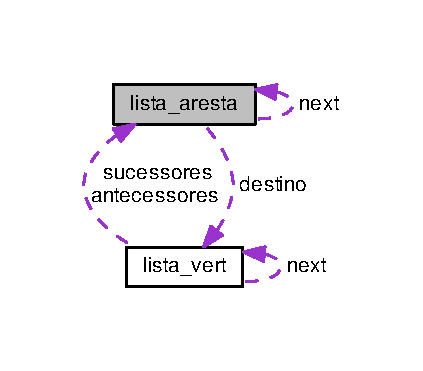
\includegraphics[width=203pt]{structlista__aresta__coll__graph}
\end{center}
\end{figure}
\subsection*{Campos de Dados}
\begin{DoxyCompactItemize}
\item 
struct \hyperlink{structlista__vert}{lista\+\_\+vert} $\ast$ \hyperlink{structlista__aresta_a324d065ab2fc1df5d59128027c4c8a5a}{destino}
\item 
int \hyperlink{structlista__aresta_aecaf90a9521bc8a80a0b67f80603b6ce}{peso}
\item 
struct \hyperlink{structlista__aresta}{lista\+\_\+aresta} $\ast$ \hyperlink{structlista__aresta_a55d9a8d5fcc901c1d8802239735b4af7}{next}
\end{DoxyCompactItemize}


\subsection{Descrição Detalhada}


Definição na linha 22 do arquivo grafo\+\_\+priv.\+h.



\subsection{Campos}
\hypertarget{structlista__aresta_a324d065ab2fc1df5d59128027c4c8a5a}{}\index{lista\+\_\+aresta@{lista\+\_\+aresta}!destino@{destino}}
\index{destino@{destino}!lista\+\_\+aresta@{lista\+\_\+aresta}}
\subsubsection[{destino}]{\setlength{\rightskip}{0pt plus 5cm}struct {\bf lista\+\_\+vert}$\ast$ lista\+\_\+aresta\+::destino}\label{structlista__aresta_a324d065ab2fc1df5d59128027c4c8a5a}


Definição na linha 23 do arquivo grafo\+\_\+priv.\+h.



Referenciado por dfs(), existe\+\_\+aresta(), inserir\+\_\+aresta(), menor\+\_\+caminho() e remover\+\_\+vert().

\hypertarget{structlista__aresta_a55d9a8d5fcc901c1d8802239735b4af7}{}\index{lista\+\_\+aresta@{lista\+\_\+aresta}!next@{next}}
\index{next@{next}!lista\+\_\+aresta@{lista\+\_\+aresta}}
\subsubsection[{next}]{\setlength{\rightskip}{0pt plus 5cm}struct {\bf lista\+\_\+aresta}$\ast$ lista\+\_\+aresta\+::next}\label{structlista__aresta_a55d9a8d5fcc901c1d8802239735b4af7}


Definição na linha 25 do arquivo grafo\+\_\+priv.\+h.



Referenciado por dfs(), existe\+\_\+aresta(), inserir\+\_\+aresta(), menor\+\_\+caminho(), num\+\_\+arestas() e remover\+\_\+aresta().

\hypertarget{structlista__aresta_aecaf90a9521bc8a80a0b67f80603b6ce}{}\index{lista\+\_\+aresta@{lista\+\_\+aresta}!peso@{peso}}
\index{peso@{peso}!lista\+\_\+aresta@{lista\+\_\+aresta}}
\subsubsection[{peso}]{\setlength{\rightskip}{0pt plus 5cm}int lista\+\_\+aresta\+::peso}\label{structlista__aresta_aecaf90a9521bc8a80a0b67f80603b6ce}


Definição na linha 24 do arquivo grafo\+\_\+priv.\+h.



Referenciado por inserir\+\_\+aresta() e menor\+\_\+caminho().



A documentação para esta estrutura foi gerada a partir do seguinte arquivo\+:\begin{DoxyCompactItemize}
\item 
/home/rafael/\+Projeto\+Final\+M\+P/\+Fase2\+Interface/include/\hyperlink{grafo__priv_8h}{grafo\+\_\+priv.\+h}\end{DoxyCompactItemize}

\hypertarget{structlista__origem}{}\section{Referência da Estrutura lista\+\_\+origem}
\label{structlista__origem}\index{lista\+\_\+origem@{lista\+\_\+origem}}


{\ttfamily \#include $<$grafo\+\_\+priv.\+h$>$}



Diagrama de colaboração para lista\+\_\+origem\+:
\nopagebreak
\begin{figure}[H]
\begin{center}
\leavevmode
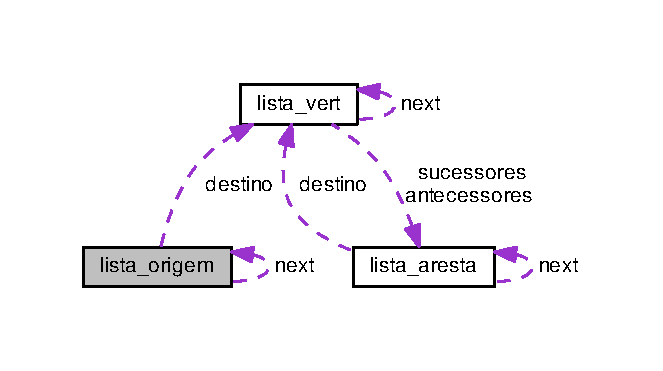
\includegraphics[width=318pt]{structlista__origem__coll__graph}
\end{center}
\end{figure}
\subsection*{Campos de Dados}
\begin{DoxyCompactItemize}
\item 
\hyperlink{grafo__priv_8h_aecb68281fecb412bf6427dd6a07d5077}{lista\+\_\+vert\+\_\+t} $\ast$ \hyperlink{structlista__origem_a2634ade77a03658b5cbc02e44d3e784f}{destino}
\item 
struct \hyperlink{structlista__origem}{lista\+\_\+origem} $\ast$ \hyperlink{structlista__origem_a3d90d523832090d0a99ee45025c95c03}{next}
\end{DoxyCompactItemize}


\subsection{Descrição Detalhada}


Definição na linha 36 do arquivo grafo\+\_\+priv.\+h.



\subsection{Campos}
\hypertarget{structlista__origem_a2634ade77a03658b5cbc02e44d3e784f}{}\index{lista\+\_\+origem@{lista\+\_\+origem}!destino@{destino}}
\index{destino@{destino}!lista\+\_\+origem@{lista\+\_\+origem}}
\subsubsection[{destino}]{\setlength{\rightskip}{0pt plus 5cm}{\bf lista\+\_\+vert\+\_\+t}$\ast$ lista\+\_\+origem\+::destino}\label{structlista__origem_a2634ade77a03658b5cbc02e44d3e784f}


Definição na linha 37 do arquivo grafo\+\_\+priv.\+h.



Referenciado por eh\+\_\+conexo(), existe\+\_\+origem(), inserir\+\_\+origem() e remover\+\_\+origem().

\hypertarget{structlista__origem_a3d90d523832090d0a99ee45025c95c03}{}\index{lista\+\_\+origem@{lista\+\_\+origem}!next@{next}}
\index{next@{next}!lista\+\_\+origem@{lista\+\_\+origem}}
\subsubsection[{next}]{\setlength{\rightskip}{0pt plus 5cm}struct {\bf lista\+\_\+origem}$\ast$ lista\+\_\+origem\+::next}\label{structlista__origem_a3d90d523832090d0a99ee45025c95c03}


Definição na linha 38 do arquivo grafo\+\_\+priv.\+h.



Referenciado por eh\+\_\+conexo(), existe\+\_\+origem(), inserir\+\_\+origem() e remover\+\_\+origem().



A documentação para esta estrutura foi gerada a partir do seguinte arquivo\+:\begin{DoxyCompactItemize}
\item 
/home/rafael/\+Projeto\+Final\+M\+P/\+Fase2\+Interface/include/\hyperlink{grafo__priv_8h}{grafo\+\_\+priv.\+h}\end{DoxyCompactItemize}

\hypertarget{structlista__vert}{}\section{Referência da Estrutura lista\+\_\+vert}
\label{structlista__vert}\index{lista\+\_\+vert@{lista\+\_\+vert}}


{\ttfamily \#include $<$grafo\+\_\+priv.\+h$>$}



Diagrama de colaboração para lista\+\_\+vert\+:\nopagebreak
\begin{figure}[H]
\begin{center}
\leavevmode
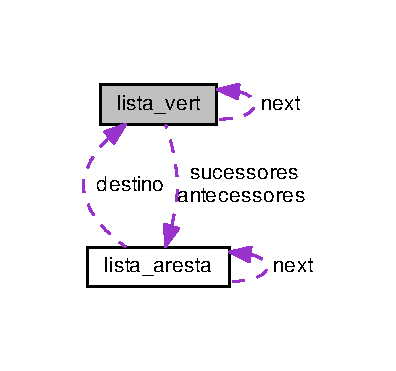
\includegraphics[width=190pt]{structlista__vert__coll__graph}
\end{center}
\end{figure}
\subsection*{Campos de Dados}
\begin{DoxyCompactItemize}
\item 
int \hyperlink{structlista__vert_acce74c81e9c5ed24ff7bc175e22a7079}{id}
\item 
int \hyperlink{structlista__vert_a4741315d4db64dad0ee3b59d8f5a4951}{id\+\_\+externo}
\item 
\hyperlink{grafo__priv_8h_a8c99b03365ae7f753c4cf1a20d9e9257}{lista\+\_\+aresta\+\_\+t} $\ast$ \hyperlink{structlista__vert_a39a423ac0ec49cb5bcca3c73c353db19}{antecessores}
\item 
\hyperlink{grafo__priv_8h_a8c99b03365ae7f753c4cf1a20d9e9257}{lista\+\_\+aresta\+\_\+t} $\ast$ \hyperlink{structlista__vert_ac003e2d2beffcf2432cac5460cf82263}{sucessores}
\item 
struct \hyperlink{structlista__vert}{lista\+\_\+vert} $\ast$ \hyperlink{structlista__vert_a772eebf412b0d7e40a73f5989e6a1835}{next}
\end{DoxyCompactItemize}


\subsection{Descrição Detalhada}


Definição na linha 28 do arquivo grafo\+\_\+priv.\+h.



\subsection{Campos}
\hypertarget{structlista__vert_a39a423ac0ec49cb5bcca3c73c353db19}{}\index{lista\+\_\+vert@{lista\+\_\+vert}!antecessores@{antecessores}}
\index{antecessores@{antecessores}!lista\+\_\+vert@{lista\+\_\+vert}}
\subsubsection[{antecessores}]{\setlength{\rightskip}{0pt plus 5cm}{\bf lista\+\_\+aresta\+\_\+t}$\ast$ lista\+\_\+vert\+::antecessores}\label{structlista__vert_a39a423ac0ec49cb5bcca3c73c353db19}


Definição na linha 31 do arquivo grafo\+\_\+priv.\+h.



Referenciado por inserir\+\_\+vert() e remover\+\_\+aresta().

\hypertarget{structlista__vert_acce74c81e9c5ed24ff7bc175e22a7079}{}\index{lista\+\_\+vert@{lista\+\_\+vert}!id@{id}}
\index{id@{id}!lista\+\_\+vert@{lista\+\_\+vert}}
\subsubsection[{id}]{\setlength{\rightskip}{0pt plus 5cm}int lista\+\_\+vert\+::id}\label{structlista__vert_acce74c81e9c5ed24ff7bc175e22a7079}


Definição na linha 29 do arquivo grafo\+\_\+priv.\+h.



Referenciado por dfs(), eh\+\_\+conexo(), inserir\+\_\+origem(), inserir\+\_\+vert(), menor\+\_\+caminho(), remover\+\_\+aresta(), remover\+\_\+origem() e remover\+\_\+vert().

\hypertarget{structlista__vert_a4741315d4db64dad0ee3b59d8f5a4951}{}\index{lista\+\_\+vert@{lista\+\_\+vert}!id\+\_\+externo@{id\+\_\+externo}}
\index{id\+\_\+externo@{id\+\_\+externo}!lista\+\_\+vert@{lista\+\_\+vert}}
\subsubsection[{id\+\_\+externo}]{\setlength{\rightskip}{0pt plus 5cm}int lista\+\_\+vert\+::id\+\_\+externo}\label{structlista__vert_a4741315d4db64dad0ee3b59d8f5a4951}


Definição na linha 30 do arquivo grafo\+\_\+priv.\+h.



Referenciado por existe\+\_\+aresta(), existe\+\_\+origem(), inserir\+\_\+vert() e remover\+\_\+vert().

\hypertarget{structlista__vert_a772eebf412b0d7e40a73f5989e6a1835}{}\index{lista\+\_\+vert@{lista\+\_\+vert}!next@{next}}
\index{next@{next}!lista\+\_\+vert@{lista\+\_\+vert}}
\subsubsection[{next}]{\setlength{\rightskip}{0pt plus 5cm}struct {\bf lista\+\_\+vert}$\ast$ lista\+\_\+vert\+::next}\label{structlista__vert_a772eebf412b0d7e40a73f5989e6a1835}


Definição na linha 33 do arquivo grafo\+\_\+priv.\+h.



Referenciado por existe\+\_\+aresta(), inserir\+\_\+aresta(), inserir\+\_\+origem(), inserir\+\_\+vert(), menor\+\_\+caminho(), num\+\_\+arestas(), num\+\_\+vert(), remover\+\_\+aresta() e remover\+\_\+vert().

\hypertarget{structlista__vert_ac003e2d2beffcf2432cac5460cf82263}{}\index{lista\+\_\+vert@{lista\+\_\+vert}!sucessores@{sucessores}}
\index{sucessores@{sucessores}!lista\+\_\+vert@{lista\+\_\+vert}}
\subsubsection[{sucessores}]{\setlength{\rightskip}{0pt plus 5cm}{\bf lista\+\_\+aresta\+\_\+t}$\ast$ lista\+\_\+vert\+::sucessores}\label{structlista__vert_ac003e2d2beffcf2432cac5460cf82263}


Definição na linha 32 do arquivo grafo\+\_\+priv.\+h.



Referenciado por dfs(), existe\+\_\+aresta(), inserir\+\_\+aresta(), inserir\+\_\+vert(), menor\+\_\+caminho(), num\+\_\+arestas() e remover\+\_\+aresta().



A documentação para esta estrutura foi gerada a partir do seguinte arquivo\+:\begin{DoxyCompactItemize}
\item 
/home/rafael/\+Projeto\+Final\+M\+P/\+Fase2\+Interface/include/\hyperlink{grafo__priv_8h}{grafo\+\_\+priv.\+h}\end{DoxyCompactItemize}

\hypertarget{structlista__vert__codigo}{}\section{Referência da Estrutura lista\+\_\+vert\+\_\+codigo}
\label{structlista__vert__codigo}\index{lista\+\_\+vert\+\_\+codigo@{lista\+\_\+vert\+\_\+codigo}}


{\ttfamily \#include $<$grafo\+\_\+priv.\+h$>$}



Diagrama de colaboração para lista\+\_\+vert\+\_\+codigo\+:
\nopagebreak
\begin{figure}[H]
\begin{center}
\leavevmode
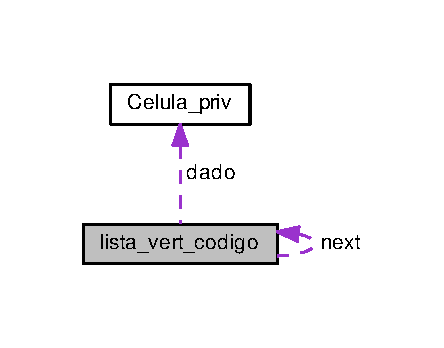
\includegraphics[width=213pt]{structlista__vert__codigo__coll__graph}
\end{center}
\end{figure}
\subsection*{Campos de Dados}
\begin{DoxyCompactItemize}
\item 
\hyperlink{grafo_8h_ac2219b5d1f94e440b5895ce440ab23b9}{Celula\+\_\+priv\+\_\+t} \hyperlink{structlista__vert__codigo_a8e51b3141307b34cb74d6433a136f73b}{dado}
\item 
int \hyperlink{structlista__vert__codigo_acc7c3bce66ab242ba6e64e763dfb63b3}{id}
\item 
struct \hyperlink{structlista__vert__codigo}{lista\+\_\+vert\+\_\+codigo} $\ast$ \hyperlink{structlista__vert__codigo_af1cac7f22cb6142a13bd1f9c41f4c0b5}{next}
\end{DoxyCompactItemize}


\subsection{Descrição Detalhada}


Definição na linha 16 do arquivo grafo\+\_\+priv.\+h.



\subsection{Campos}
\hypertarget{structlista__vert__codigo_a8e51b3141307b34cb74d6433a136f73b}{}\index{lista\+\_\+vert\+\_\+codigo@{lista\+\_\+vert\+\_\+codigo}!dado@{dado}}
\index{dado@{dado}!lista\+\_\+vert\+\_\+codigo@{lista\+\_\+vert\+\_\+codigo}}
\subsubsection[{dado}]{\setlength{\rightskip}{0pt plus 5cm}{\bf Celula\+\_\+priv\+\_\+t} lista\+\_\+vert\+\_\+codigo\+::dado}\label{structlista__vert__codigo_a8e51b3141307b34cb74d6433a136f73b}


Definição na linha 17 do arquivo grafo\+\_\+priv.\+h.



Referenciado por achar\+\_\+celula(), achar\+\_\+id(), existe\+\_\+vert(), Grava\+\_\+\+Arq() e Imprime\+\_\+\+Tarefas().

\hypertarget{structlista__vert__codigo_acc7c3bce66ab242ba6e64e763dfb63b3}{}\index{lista\+\_\+vert\+\_\+codigo@{lista\+\_\+vert\+\_\+codigo}!id@{id}}
\index{id@{id}!lista\+\_\+vert\+\_\+codigo@{lista\+\_\+vert\+\_\+codigo}}
\subsubsection[{id}]{\setlength{\rightskip}{0pt plus 5cm}int lista\+\_\+vert\+\_\+codigo\+::id}\label{structlista__vert__codigo_acc7c3bce66ab242ba6e64e763dfb63b3}


Definição na linha 18 do arquivo grafo\+\_\+priv.\+h.



Referenciado por achar\+\_\+id(), inserir\+\_\+vert(), ja\+\_\+feito(), maior\+\_\+id() e remover\+\_\+vert().

\hypertarget{structlista__vert__codigo_af1cac7f22cb6142a13bd1f9c41f4c0b5}{}\index{lista\+\_\+vert\+\_\+codigo@{lista\+\_\+vert\+\_\+codigo}!next@{next}}
\index{next@{next}!lista\+\_\+vert\+\_\+codigo@{lista\+\_\+vert\+\_\+codigo}}
\subsubsection[{next}]{\setlength{\rightskip}{0pt plus 5cm}struct {\bf lista\+\_\+vert\+\_\+codigo}$\ast$ lista\+\_\+vert\+\_\+codigo\+::next}\label{structlista__vert__codigo_af1cac7f22cb6142a13bd1f9c41f4c0b5}


Definição na linha 19 do arquivo grafo\+\_\+priv.\+h.



Referenciado por achar\+\_\+celula(), achar\+\_\+id(), existe\+\_\+vert(), Grava\+\_\+\+Arq(), Imprime\+\_\+\+Tarefas(), inserir\+\_\+vert(), ja\+\_\+feito(), maior\+\_\+id() e remover\+\_\+vert().



A documentação para esta estrutura foi gerada a partir do seguinte arquivo\+:\begin{DoxyCompactItemize}
\item 
/home/rafael/\+Projeto\+Final\+M\+P/\+Fase2\+Interface/include/\hyperlink{grafo__priv_8h}{grafo\+\_\+priv.\+h}\end{DoxyCompactItemize}

\chapter{Arquivos}
\hypertarget{grafo_8h}{}\section{Referência do Arquivo /home/rafael/\+Projeto\+Final\+M\+P/\+Fase2\+Interface/include/grafo.h}
\label{grafo_8h}\index{/home/rafael/\+Projeto\+Final\+M\+P/\+Fase2\+Interface/include/grafo.\+h@{/home/rafael/\+Projeto\+Final\+M\+P/\+Fase2\+Interface/include/grafo.\+h}}


Define funções usadas pelo usuario.  


Este grafo mostra quais arquivos estão direta ou indiretamente relacionados com este arquivo\+:\nopagebreak
\begin{figure}[H]
\begin{center}
\leavevmode
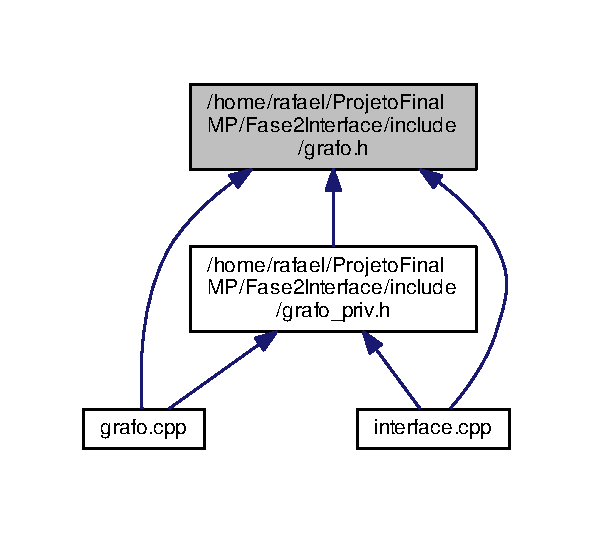
\includegraphics[width=285pt]{grafo_8h__dep__incl}
\end{center}
\end{figure}
\subsection*{Definições de Tipos}
\begin{DoxyCompactItemize}
\item 
typedef enum \hyperlink{grafo_8h_a4a2eceb977b50eb0028c419047e56e1d}{resp} \hyperlink{grafo_8h_a64f906a639abdfda7fffa9ace7e4c286}{resposta}
\item 
typedef struct \hyperlink{structgrafo__priv}{grafo\+\_\+priv} \hyperlink{grafo_8h_a282167c584dceb79dde5c159a85b685b}{grafo\+\_\+priv\+\_\+t}
\item 
typedef struct \hyperlink{structCelula__priv}{Celula\+\_\+priv} \hyperlink{grafo_8h_ac2219b5d1f94e440b5895ce440ab23b9}{Celula\+\_\+priv\+\_\+t}
\end{DoxyCompactItemize}
\subsection*{Enumerações}
\begin{DoxyCompactItemize}
\item 
enum \hyperlink{grafo_8h_a4a2eceb977b50eb0028c419047e56e1d}{resp} \{ \hyperlink{grafo_8h_a4a2eceb977b50eb0028c419047e56e1da18eca9337ac663e3309296308db9dcd7}{F\+A\+L\+S\+E\+\_\+\+T}, 
\hyperlink{grafo_8h_a4a2eceb977b50eb0028c419047e56e1da5cb1a0e1a9975a61106e3b540ca4c0ad}{T\+R\+U\+E\+\_\+\+T}
 \}
\end{DoxyCompactItemize}
\subsection*{Funções}
\begin{DoxyCompactItemize}
\item 
\hyperlink{grafo_8h_a282167c584dceb79dde5c159a85b685b}{grafo\+\_\+priv\+\_\+t} $\ast$ \hyperlink{grafo_8h_a3e61bf2ada0f9af7e2e9883241496606}{criar\+\_\+grafo} (void)
\begin{DoxyCompactList}\small\item\em Cria grafo. \end{DoxyCompactList}\item 
\hyperlink{grafo_8h_a282167c584dceb79dde5c159a85b685b}{grafo\+\_\+priv\+\_\+t} $\ast$ \hyperlink{grafo_8h_af4f0fbcdd746c0f494e9601a83ddc9fe}{deletar\+\_\+grafo} (\hyperlink{grafo_8h_a282167c584dceb79dde5c159a85b685b}{grafo\+\_\+priv\+\_\+t} $\ast$meu\+\_\+grafo)
\begin{DoxyCompactList}\small\item\em Deleta grafo. \end{DoxyCompactList}\item 
\hyperlink{grafo_8h_a64f906a639abdfda7fffa9ace7e4c286}{resposta} \hyperlink{grafo_8h_ac70f5a4fd6ff7c6913f0ce99de099263}{existe\+\_\+vert} (const \hyperlink{grafo_8h_a282167c584dceb79dde5c159a85b685b}{grafo\+\_\+priv\+\_\+t} $\ast$meu\+\_\+grafo, int id\+\_\+externo)
\item 
\hyperlink{grafo_8h_ac2219b5d1f94e440b5895ce440ab23b9}{Celula\+\_\+priv\+\_\+t} $\ast$ \hyperlink{grafo_8h_a28b6414a2684992da035d5605178c770}{cria\+\_\+celula} (int id\+\_\+externo, int executada, int duracao, int ini\+\_\+min, int pre\+\_\+req, int $\ast$reqs, const char $\ast$nome)
\item 
\hyperlink{grafo_8h_a64f906a639abdfda7fffa9ace7e4c286}{resposta} \hyperlink{grafo_8h_a56edc294bdf9e834989d9c8d31ed3a64}{existe\+\_\+aresta} (const \hyperlink{grafo_8h_a282167c584dceb79dde5c159a85b685b}{grafo\+\_\+priv\+\_\+t} $\ast$meu\+\_\+grafo, int id\+\_\+externo1, int id\+\_\+externo2)
\item 
int \hyperlink{grafo_8h_ac428ee7436d16b5251b093aa79183fda}{achar\+\_\+id} (const \hyperlink{grafo_8h_a282167c584dceb79dde5c159a85b685b}{grafo\+\_\+priv\+\_\+t} $\ast$meu\+\_\+grafo, int id\+\_\+externo)
\item 
\hyperlink{grafo_8h_ac2219b5d1f94e440b5895ce440ab23b9}{Celula\+\_\+priv\+\_\+t} $\ast$ \hyperlink{grafo_8h_a90390d2135067928e2c69cd964c9bec5}{achar\+\_\+celula} (const \hyperlink{grafo_8h_a282167c584dceb79dde5c159a85b685b}{grafo\+\_\+priv\+\_\+t} $\ast$meu\+\_\+grafo, int id\+\_\+externo)
\item 
void \hyperlink{grafo_8h_a659b567cb7e165b526b6fe05a433452e}{inserir\+\_\+vert} (\hyperlink{grafo_8h_a282167c584dceb79dde5c159a85b685b}{grafo\+\_\+priv\+\_\+t} $\ast$meu\+\_\+grafo, \hyperlink{grafo_8h_ac2219b5d1f94e440b5895ce440ab23b9}{Celula\+\_\+priv\+\_\+t} $\ast$celula)
\item 
void \hyperlink{grafo_8h_a0e69707897c891bf77319d494cae8f26}{inserir\+\_\+aresta} (\hyperlink{grafo_8h_a282167c584dceb79dde5c159a85b685b}{grafo\+\_\+priv\+\_\+t} $\ast$meu\+\_\+grafo, int id\+\_\+externo1, \hyperlink{grafo_8h_ac2219b5d1f94e440b5895ce440ab23b9}{Celula\+\_\+priv\+\_\+t} $\ast$celula2, int peso)
\item 
void \hyperlink{grafo_8h_a2812c8a1cbeaab16d0aaa6da10ec4372}{remover\+\_\+vert} (\hyperlink{grafo_8h_a282167c584dceb79dde5c159a85b685b}{grafo\+\_\+priv\+\_\+t} $\ast$meu\+\_\+grafo, int id\+\_\+externo)
\item 
void \hyperlink{grafo_8h_ac16199e4256247b546b67d6d881be137}{remover\+\_\+aresta} (\hyperlink{grafo_8h_a282167c584dceb79dde5c159a85b685b}{grafo\+\_\+priv\+\_\+t} $\ast$meu\+\_\+grafo, int id\+\_\+externo1, int id\+\_\+externo2)
\item 
int \hyperlink{grafo_8h_a5bedfb800e326da354b0403421e0d1ef}{maior\+\_\+id} (const \hyperlink{grafo_8h_a282167c584dceb79dde5c159a85b685b}{grafo\+\_\+priv\+\_\+t} $\ast$meu\+\_\+grafo)
\item 
int \hyperlink{grafo_8h_a31c64875fe3134ba04439feb7d119cf3}{num\+\_\+vert} (const \hyperlink{grafo_8h_a282167c584dceb79dde5c159a85b685b}{grafo\+\_\+priv\+\_\+t} $\ast$meu\+\_\+grafo)
\item 
int \hyperlink{grafo_8h_ac94be03e94792b9b868abb38c7e17e36}{num\+\_\+arestas} (const \hyperlink{grafo_8h_a282167c584dceb79dde5c159a85b685b}{grafo\+\_\+priv\+\_\+t} $\ast$meu\+\_\+grafo)
\item 
int \hyperlink{grafo_8h_ad507a38f9feef6cad69436ec774b535f}{menor\+\_\+caminho} (const \hyperlink{grafo_8h_a282167c584dceb79dde5c159a85b685b}{grafo\+\_\+priv\+\_\+t} $\ast$meu\+\_\+grafo, int $\ast$$\ast$dist)
\item 
\hyperlink{grafo_8h_a64f906a639abdfda7fffa9ace7e4c286}{resposta} \hyperlink{grafo_8h_a46f8363c4da6edf056e5fffba46e1bc7}{eh\+\_\+conexo} (const \hyperlink{grafo_8h_a282167c584dceb79dde5c159a85b685b}{grafo\+\_\+priv\+\_\+t} $\ast$meu\+\_\+grafo)
\item 
int \hyperlink{grafo_8h_a14183876086781302e2d81ab2457dc4e}{tempo\+\_\+minimo} (const \hyperlink{grafo_8h_a282167c584dceb79dde5c159a85b685b}{grafo\+\_\+priv\+\_\+t} $\ast$meu\+\_\+grafo, int id\+\_\+fim)
\item 
void \hyperlink{grafo_8h_acb5b55f7d1508a1b35b76e43bc817623}{ja\+\_\+feito} (const \hyperlink{grafo_8h_a282167c584dceb79dde5c159a85b685b}{grafo\+\_\+priv\+\_\+t} $\ast$meu\+\_\+grafo, int d)
\item 
void \hyperlink{grafo_8h_acd0aa806c04807a2b8086bd7a6c59b50}{Ler\+\_\+\+Tarefas} (\hyperlink{grafo_8h_a282167c584dceb79dde5c159a85b685b}{grafo\+\_\+priv\+\_\+t} $\ast$meu\+\_\+grafo, \hyperlink{grafo_8h_ac2219b5d1f94e440b5895ce440ab23b9}{Celula\+\_\+priv\+\_\+t} $\ast$celula, const char $\ast$Nome\+Arq)
\item 
void \hyperlink{grafo_8h_a79154a07716d283ad68106cf54beaf07}{editar\+\_\+celula} (\hyperlink{grafo_8h_a282167c584dceb79dde5c159a85b685b}{grafo\+\_\+priv\+\_\+t} $\ast$meu\+\_\+grafo, int I\+D)
\item 
void \hyperlink{grafo_8h_a1dd7cc6696ade339827db4d2019239fc}{Imprime\+\_\+\+Tarefas} (const \hyperlink{grafo_8h_a282167c584dceb79dde5c159a85b685b}{grafo\+\_\+priv\+\_\+t} $\ast$meu\+\_\+grafo, int linha, int coluna)
\item 
void \hyperlink{grafo_8h_aadbd57b376954aeeb119120d5a4a196f}{Grava\+\_\+\+Arq} (\hyperlink{grafo_8h_a282167c584dceb79dde5c159a85b685b}{grafo\+\_\+priv\+\_\+t} $\ast$meu\+\_\+grafo, char $\ast$Nome\+Arq)
\item 
\hyperlink{grafo_8h_a282167c584dceb79dde5c159a85b685b}{grafo\+\_\+priv\+\_\+t} $\ast$ \hyperlink{grafo_8h_a1bb7038cecd5aa54025b6c5931bc0205}{cria\+Grafo\+Arq} (char $\ast$nome\+Arq)
\end{DoxyCompactItemize}


\subsection{Descrição Detalhada}
Define funções usadas pelo usuario. 



\subsection{Definições dos tipos}
\hypertarget{grafo_8h_ac2219b5d1f94e440b5895ce440ab23b9}{}\index{grafo.\+h@{grafo.\+h}!Celula\+\_\+priv\+\_\+t@{Celula\+\_\+priv\+\_\+t}}
\index{Celula\+\_\+priv\+\_\+t@{Celula\+\_\+priv\+\_\+t}!grafo.\+h@{grafo.\+h}}
\subsubsection[{Celula\+\_\+priv\+\_\+t}]{\setlength{\rightskip}{0pt plus 5cm}typedef struct {\bf Celula\+\_\+priv} {\bf Celula\+\_\+priv\+\_\+t}}\label{grafo_8h_ac2219b5d1f94e440b5895ce440ab23b9}


Definição na linha 19 do arquivo grafo.\+h.

\hypertarget{grafo_8h_a282167c584dceb79dde5c159a85b685b}{}\index{grafo.\+h@{grafo.\+h}!grafo\+\_\+priv\+\_\+t@{grafo\+\_\+priv\+\_\+t}}
\index{grafo\+\_\+priv\+\_\+t@{grafo\+\_\+priv\+\_\+t}!grafo.\+h@{grafo.\+h}}
\subsubsection[{grafo\+\_\+priv\+\_\+t}]{\setlength{\rightskip}{0pt plus 5cm}typedef struct {\bf grafo\+\_\+priv} {\bf grafo\+\_\+priv\+\_\+t}}\label{grafo_8h_a282167c584dceb79dde5c159a85b685b}


Definição na linha 17 do arquivo grafo.\+h.

\hypertarget{grafo_8h_a64f906a639abdfda7fffa9ace7e4c286}{}\index{grafo.\+h@{grafo.\+h}!resposta@{resposta}}
\index{resposta@{resposta}!grafo.\+h@{grafo.\+h}}
\subsubsection[{resposta}]{\setlength{\rightskip}{0pt plus 5cm}typedef enum {\bf resp}  {\bf resposta}}\label{grafo_8h_a64f906a639abdfda7fffa9ace7e4c286}


\subsection{Enumerações}
\hypertarget{grafo_8h_a4a2eceb977b50eb0028c419047e56e1d}{}\index{grafo.\+h@{grafo.\+h}!resp@{resp}}
\index{resp@{resp}!grafo.\+h@{grafo.\+h}}
\subsubsection[{resp}]{\setlength{\rightskip}{0pt plus 5cm}enum {\bf resp}}\label{grafo_8h_a4a2eceb977b50eb0028c419047e56e1d}
\begin{Desc}
\item[Valores de enumerações]\par
\begin{description}
\index{F\+A\+L\+S\+E\+\_\+\+T@{F\+A\+L\+S\+E\+\_\+\+T}!grafo.\+h@{grafo.\+h}}\index{grafo.\+h@{grafo.\+h}!F\+A\+L\+S\+E\+\_\+\+T@{F\+A\+L\+S\+E\+\_\+\+T}}\item[{\em 
\hypertarget{grafo_8h_a4a2eceb977b50eb0028c419047e56e1da18eca9337ac663e3309296308db9dcd7}{}F\+A\+L\+S\+E\+\_\+\+T\label{grafo_8h_a4a2eceb977b50eb0028c419047e56e1da18eca9337ac663e3309296308db9dcd7}
}]\index{T\+R\+U\+E\+\_\+\+T@{T\+R\+U\+E\+\_\+\+T}!grafo.\+h@{grafo.\+h}}\index{grafo.\+h@{grafo.\+h}!T\+R\+U\+E\+\_\+\+T@{T\+R\+U\+E\+\_\+\+T}}\item[{\em 
\hypertarget{grafo_8h_a4a2eceb977b50eb0028c419047e56e1da5cb1a0e1a9975a61106e3b540ca4c0ad}{}T\+R\+U\+E\+\_\+\+T\label{grafo_8h_a4a2eceb977b50eb0028c419047e56e1da5cb1a0e1a9975a61106e3b540ca4c0ad}
}]\end{description}
\end{Desc}


Definição na linha 9 do arquivo grafo.\+h.



\subsection{Funções}
\hypertarget{grafo_8h_a90390d2135067928e2c69cd964c9bec5}{}\index{grafo.\+h@{grafo.\+h}!achar\+\_\+celula@{achar\+\_\+celula}}
\index{achar\+\_\+celula@{achar\+\_\+celula}!grafo.\+h@{grafo.\+h}}
\subsubsection[{achar\+\_\+celula(const grafo\+\_\+priv\+\_\+t $\ast$meu\+\_\+grafo, int id\+\_\+externo)}]{\setlength{\rightskip}{0pt plus 5cm}{\bf Celula\+\_\+priv\+\_\+t}$\ast$ achar\+\_\+celula (
\begin{DoxyParamCaption}
\item[{const {\bf grafo\+\_\+priv\+\_\+t} $\ast$}]{meu\+\_\+grafo, }
\item[{int}]{id\+\_\+externo}
\end{DoxyParamCaption}
)}\label{grafo_8h_a90390d2135067928e2c69cd964c9bec5}


Definição na linha 117 do arquivo grafo.\+cpp.



Referências lista\+\_\+vert\+\_\+codigo\+::dado, Celula\+\_\+priv\+::id\+\_\+externo, lista\+\_\+vert\+\_\+codigo\+::next e grafo\+\_\+priv\+::tabela.



Referenciado por editar\+\_\+celula(), interface\+\_\+vizualizar\+\_\+determinada\+\_\+tarefa() e menor\+\_\+caminho().



Este é o diagrama das funções que utilizam esta função\+:\nopagebreak
\begin{figure}[H]
\begin{center}
\leavevmode
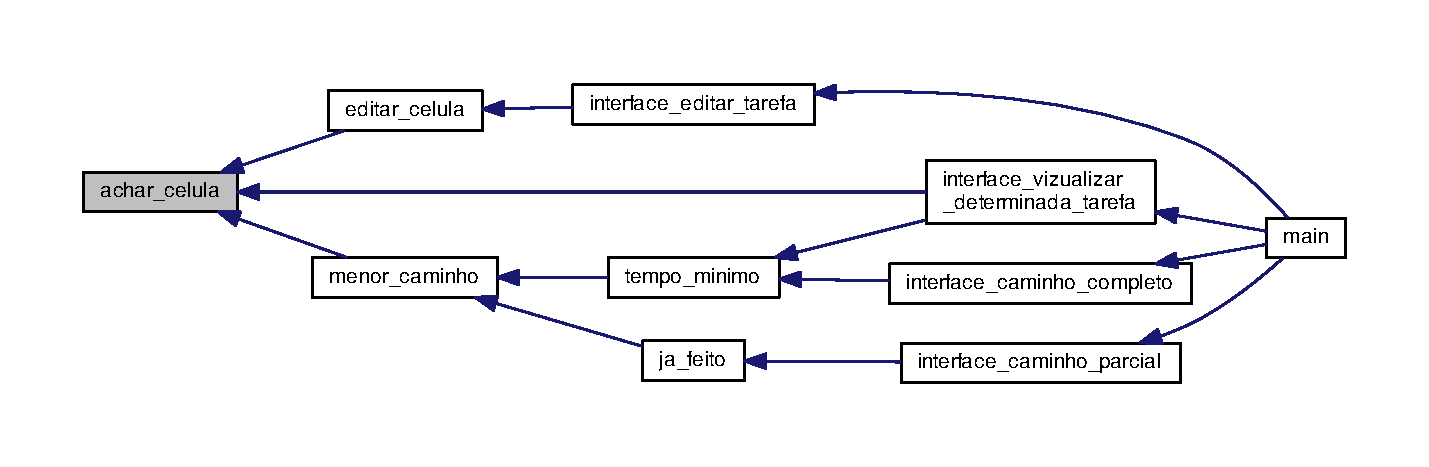
\includegraphics[width=350pt]{grafo_8h_a90390d2135067928e2c69cd964c9bec5_icgraph}
\end{center}
\end{figure}


\hypertarget{grafo_8h_ac428ee7436d16b5251b093aa79183fda}{}\index{grafo.\+h@{grafo.\+h}!achar\+\_\+id@{achar\+\_\+id}}
\index{achar\+\_\+id@{achar\+\_\+id}!grafo.\+h@{grafo.\+h}}
\subsubsection[{achar\+\_\+id(const grafo\+\_\+priv\+\_\+t $\ast$meu\+\_\+grafo, int id\+\_\+externo)}]{\setlength{\rightskip}{0pt plus 5cm}int achar\+\_\+id (
\begin{DoxyParamCaption}
\item[{const {\bf grafo\+\_\+priv\+\_\+t} $\ast$}]{meu\+\_\+grafo, }
\item[{int}]{id\+\_\+externo}
\end{DoxyParamCaption}
)}\label{grafo_8h_ac428ee7436d16b5251b093aa79183fda}


Definição na linha 107 do arquivo grafo.\+cpp.



Referências lista\+\_\+vert\+\_\+codigo\+::dado, lista\+\_\+vert\+\_\+codigo\+::id, Celula\+\_\+priv\+::id\+\_\+externo, lista\+\_\+vert\+\_\+codigo\+::next e grafo\+\_\+priv\+::tabela.



Referenciado por inserir\+\_\+aresta(), inserir\+\_\+origem(), menor\+\_\+caminho(), remover\+\_\+aresta(), remover\+\_\+origem() e remover\+\_\+vert().



Este é o diagrama das funções que utilizam esta função\+:
\nopagebreak
\begin{figure}[H]
\begin{center}
\leavevmode
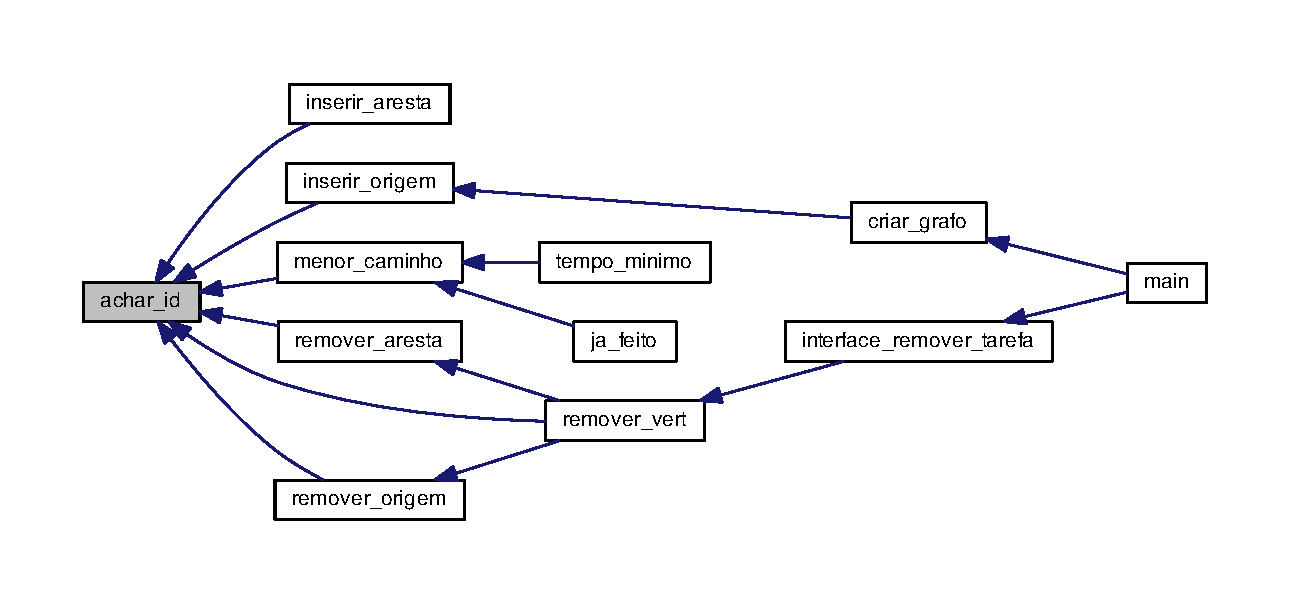
\includegraphics[width=350pt]{grafo_8h_ac428ee7436d16b5251b093aa79183fda_icgraph}
\end{center}
\end{figure}


\hypertarget{grafo_8h_a28b6414a2684992da035d5605178c770}{}\index{grafo.\+h@{grafo.\+h}!cria\+\_\+celula@{cria\+\_\+celula}}
\index{cria\+\_\+celula@{cria\+\_\+celula}!grafo.\+h@{grafo.\+h}}
\subsubsection[{cria\+\_\+celula(int id\+\_\+externo, int executada, int duracao, int ini\+\_\+min, int pre\+\_\+req, int $\ast$reqs, const char $\ast$nome)}]{\setlength{\rightskip}{0pt plus 5cm}{\bf Celula\+\_\+priv\+\_\+t}$\ast$ cria\+\_\+celula (
\begin{DoxyParamCaption}
\item[{int}]{id\+\_\+externo, }
\item[{int}]{executada, }
\item[{int}]{duracao, }
\item[{int}]{ini\+\_\+min, }
\item[{int}]{pre\+\_\+req, }
\item[{int $\ast$}]{reqs, }
\item[{const char $\ast$}]{nome}
\end{DoxyParamCaption}
)}\label{grafo_8h_a28b6414a2684992da035d5605178c770}


Definição na linha 43 do arquivo grafo.\+cpp.



Referências Celula\+\_\+priv\+::duracao, Celula\+\_\+priv\+::executada, Celula\+\_\+priv\+::id\+\_\+externo, Celula\+\_\+priv\+::ini\+\_\+min, Celula\+\_\+priv\+::nome, Celula\+\_\+priv\+::pre\+\_\+req e Celula\+\_\+priv\+::reqs.

\hypertarget{grafo_8h_a1bb7038cecd5aa54025b6c5931bc0205}{}\index{grafo.\+h@{grafo.\+h}!cria\+Grafo\+Arq@{cria\+Grafo\+Arq}}
\index{cria\+Grafo\+Arq@{cria\+Grafo\+Arq}!grafo.\+h@{grafo.\+h}}
\subsubsection[{cria\+Grafo\+Arq(char $\ast$nome\+Arq)}]{\setlength{\rightskip}{0pt plus 5cm}{\bf grafo\+\_\+priv\+\_\+t}$\ast$ cria\+Grafo\+Arq (
\begin{DoxyParamCaption}
\item[{char $\ast$}]{nome\+Arq}
\end{DoxyParamCaption}
)}\label{grafo_8h_a1bb7038cecd5aa54025b6c5931bc0205}


Definição na linha 753 do arquivo grafo.\+cpp.



Referências criar\+\_\+grafo(), Celula\+\_\+priv\+::duracao, Celula\+\_\+priv\+::executada, Celula\+\_\+priv\+::id\+\_\+externo, Celula\+\_\+priv\+::ini\+\_\+min, inserir\+\_\+aresta(), inserir\+\_\+vert(), Celula\+\_\+priv\+::nome, Celula\+\_\+priv\+::pre\+\_\+req e Celula\+\_\+priv\+::reqs.



Referenciado por main().



Este é o diagrama das funções utilizadas por esta função\+:\nopagebreak
\begin{figure}[H]
\begin{center}
\leavevmode
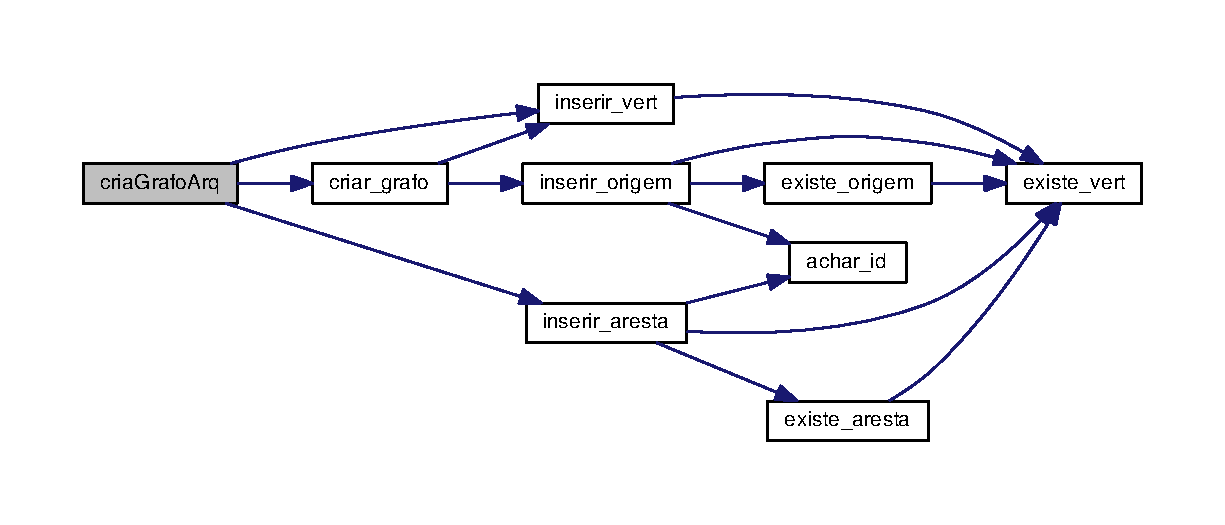
\includegraphics[width=350pt]{grafo_8h_a1bb7038cecd5aa54025b6c5931bc0205_cgraph}
\end{center}
\end{figure}




Este é o diagrama das funções que utilizam esta função\+:\nopagebreak
\begin{figure}[H]
\begin{center}
\leavevmode
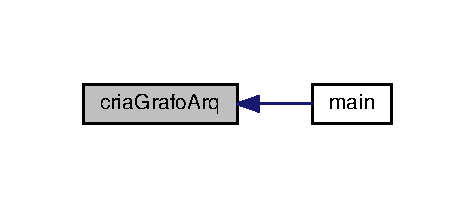
\includegraphics[width=228pt]{grafo_8h_a1bb7038cecd5aa54025b6c5931bc0205_icgraph}
\end{center}
\end{figure}


\hypertarget{grafo_8h_a3e61bf2ada0f9af7e2e9883241496606}{}\index{grafo.\+h@{grafo.\+h}!criar\+\_\+grafo@{criar\+\_\+grafo}}
\index{criar\+\_\+grafo@{criar\+\_\+grafo}!grafo.\+h@{grafo.\+h}}
\subsubsection[{criar\+\_\+grafo(void)}]{\setlength{\rightskip}{0pt plus 5cm}{\bf grafo\+\_\+priv\+\_\+t}$\ast$ criar\+\_\+grafo (
\begin{DoxyParamCaption}
\item[{void}]{}
\end{DoxyParamCaption}
)}\label{grafo_8h_a3e61bf2ada0f9af7e2e9883241496606}


Cria grafo. 

\hypertarget{grafo_8cpp_desc}{}\subsection{Descrição}\label{grafo_8cpp_desc}
Aloca a memória necessária e inicializa um grafo \hypertarget{grafo_8cpp_para}{}\subsection{Parâmetros}\label{grafo_8cpp_para}
Não ha parâmetros, a alocação e inicializam não dependem de nenhum parâmetro do usuário

\begin{DoxyReturn}{Retorna}
Se retorna um ponteiro para a grafo criado
\end{DoxyReturn}
\hypertarget{grafo_8cpp_assert}{}\subsection{Assertiva de saída}\label{grafo_8cpp_assert}
O grafo gerado é consistente e não possui nenhum vértice, origem ou aresta. 

Definição na linha 12 do arquivo grafo.\+cpp.



Referências Celula\+\_\+priv\+::executada, Celula\+\_\+priv\+::id\+\_\+externo, Celula\+\_\+priv\+::ini\+\_\+min, inserir\+\_\+origem(), inserir\+\_\+vert(), Celula\+\_\+priv\+::nome, grafo\+\_\+priv\+::origem, Celula\+\_\+priv\+::pre\+\_\+req, grafo\+\_\+priv\+::tabela e grafo\+\_\+priv\+::vert.



Referenciado por cria\+Grafo\+Arq().



Este é o diagrama das funções utilizadas por esta função\+:\nopagebreak
\begin{figure}[H]
\begin{center}
\leavevmode
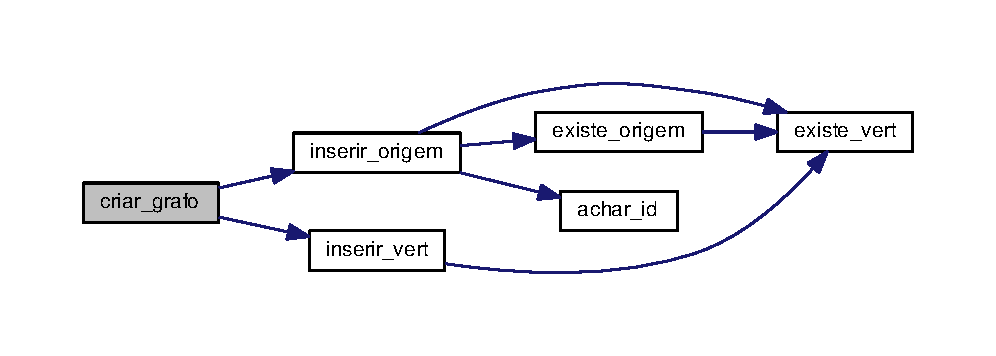
\includegraphics[width=350pt]{grafo_8h_a3e61bf2ada0f9af7e2e9883241496606_cgraph}
\end{center}
\end{figure}




Este é o diagrama das funções que utilizam esta função\+:\nopagebreak
\begin{figure}[H]
\begin{center}
\leavevmode
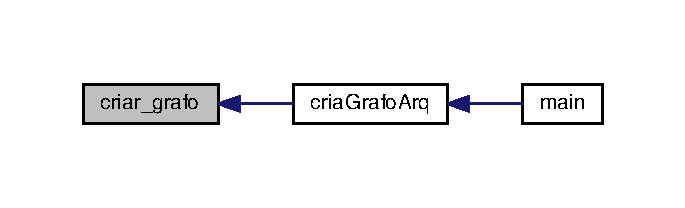
\includegraphics[width=329pt]{grafo_8h_a3e61bf2ada0f9af7e2e9883241496606_icgraph}
\end{center}
\end{figure}


\hypertarget{grafo_8h_af4f0fbcdd746c0f494e9601a83ddc9fe}{}\index{grafo.\+h@{grafo.\+h}!deletar\+\_\+grafo@{deletar\+\_\+grafo}}
\index{deletar\+\_\+grafo@{deletar\+\_\+grafo}!grafo.\+h@{grafo.\+h}}
\subsubsection[{deletar\+\_\+grafo(grafo\+\_\+priv\+\_\+t $\ast$meu\+\_\+grafo)}]{\setlength{\rightskip}{0pt plus 5cm}{\bf grafo\+\_\+priv\+\_\+t}$\ast$ deletar\+\_\+grafo (
\begin{DoxyParamCaption}
\item[{{\bf grafo\+\_\+priv\+\_\+t} $\ast$}]{meu\+\_\+grafo}
\end{DoxyParamCaption}
)}\label{grafo_8h_af4f0fbcdd746c0f494e9601a83ddc9fe}


Deleta grafo. 

\hypertarget{grafo_8cpp_desc}{}\subsection{Descrição}\label{grafo_8cpp_desc}
Desaloca toda a memória utilizada pelo grafo


\begin{DoxyParams}{Parâmetros}
{\em meu\+\_\+grafo} & -\/ Deve ser passado um ponteiro para um grafo inicializado\\
\hline
\end{DoxyParams}
\begin{DoxyReturn}{Retorna}
Retorna um ponteiro para o grafo, que será N\+U\+L\+L. O valor de retorno é muito importante, uma vez que se ele não for utilizado o grafo do usuário apontará para um endereço não alocado e qualquer tentativa de utilizá-\/lo poderá gerar erros no sistema. Caso o grafo passado não tenha sido inicializado, o programa poderá parar a execução
\end{DoxyReturn}
\hypertarget{grafo_8cpp_assert}{}\subsection{Assertiva de saída}\label{grafo_8cpp_assert}
O grafo já deve ter sido inicializado por \hyperlink{grafo_8h_a3e61bf2ada0f9af7e2e9883241496606}{criar\+\_\+grafo()} Assertiva de saída Se retornará um ponteiro para o mesmo grafo passado, após a deleção que será N\+U\+L\+L. 

Definição na linha 32 do arquivo grafo.\+cpp.



Referências lista\+\_\+vert\+\_\+codigo\+::dado, Celula\+\_\+priv\+::id\+\_\+externo, remover\+\_\+vert() e grafo\+\_\+priv\+::tabela.



Este é o diagrama das funções utilizadas por esta função\+:
\nopagebreak
\begin{figure}[H]
\begin{center}
\leavevmode
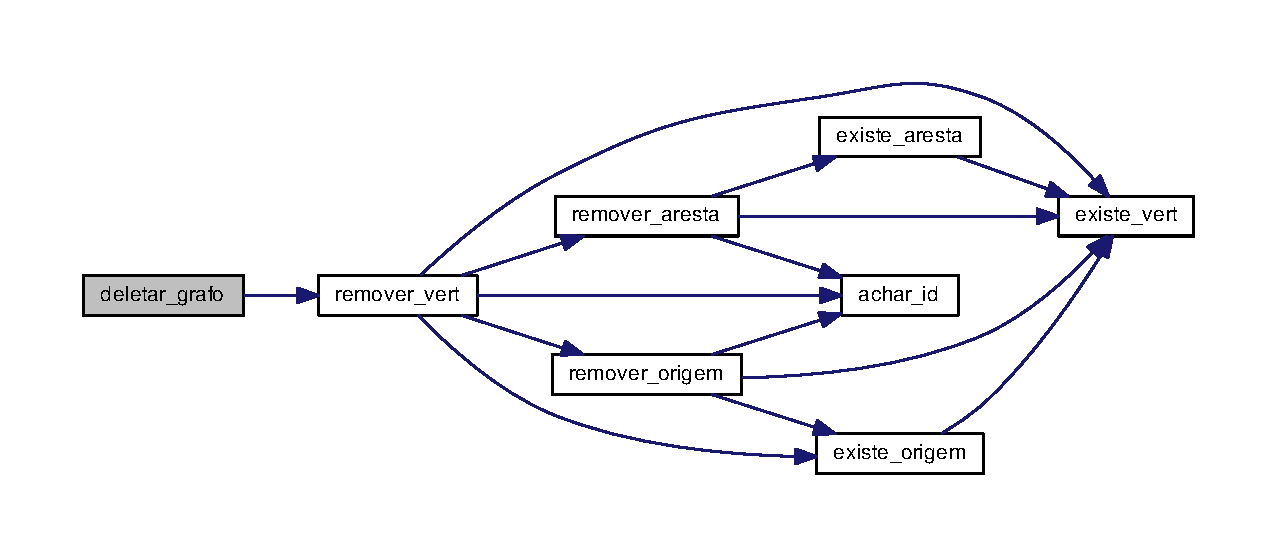
\includegraphics[width=350pt]{grafo_8h_af4f0fbcdd746c0f494e9601a83ddc9fe_cgraph}
\end{center}
\end{figure}


\hypertarget{grafo_8h_a79154a07716d283ad68106cf54beaf07}{}\index{grafo.\+h@{grafo.\+h}!editar\+\_\+celula@{editar\+\_\+celula}}
\index{editar\+\_\+celula@{editar\+\_\+celula}!grafo.\+h@{grafo.\+h}}
\subsubsection[{editar\+\_\+celula(grafo\+\_\+priv\+\_\+t $\ast$meu\+\_\+grafo, int I\+D)}]{\setlength{\rightskip}{0pt plus 5cm}void editar\+\_\+celula (
\begin{DoxyParamCaption}
\item[{{\bf grafo\+\_\+priv\+\_\+t} $\ast$}]{meu\+\_\+grafo, }
\item[{int}]{I\+D}
\end{DoxyParamCaption}
)}\label{grafo_8h_a79154a07716d283ad68106cf54beaf07}


Definição na linha 662 do arquivo grafo.\+cpp.



Referências achar\+\_\+celula(), Celula\+\_\+priv\+::duracao, Celula\+\_\+priv\+::executada, Celula\+\_\+priv\+::id\+\_\+externo, Celula\+\_\+priv\+::ini\+\_\+min, Celula\+\_\+priv\+::nome, Celula\+\_\+priv\+::pre\+\_\+req e Celula\+\_\+priv\+::reqs.



Referenciado por interface\+\_\+editar\+\_\+tarefa().



Este é o diagrama das funções utilizadas por esta função\+:\nopagebreak
\begin{figure}[H]
\begin{center}
\leavevmode
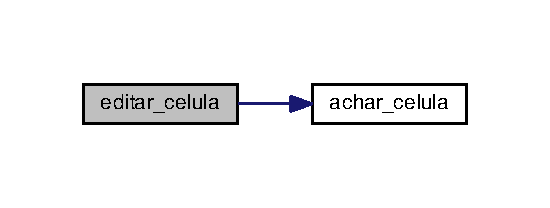
\includegraphics[width=264pt]{grafo_8h_a79154a07716d283ad68106cf54beaf07_cgraph}
\end{center}
\end{figure}




Este é o diagrama das funções que utilizam esta função\+:\nopagebreak
\begin{figure}[H]
\begin{center}
\leavevmode
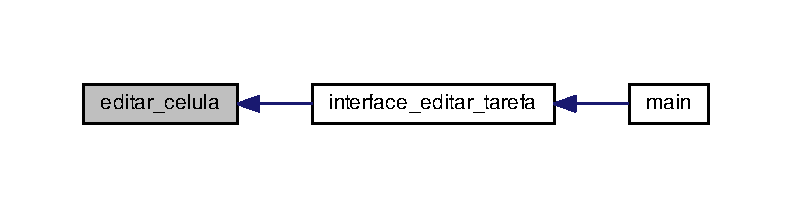
\includegraphics[width=350pt]{grafo_8h_a79154a07716d283ad68106cf54beaf07_icgraph}
\end{center}
\end{figure}


\hypertarget{grafo_8h_a46f8363c4da6edf056e5fffba46e1bc7}{}\index{grafo.\+h@{grafo.\+h}!eh\+\_\+conexo@{eh\+\_\+conexo}}
\index{eh\+\_\+conexo@{eh\+\_\+conexo}!grafo.\+h@{grafo.\+h}}
\subsubsection[{eh\+\_\+conexo(const grafo\+\_\+priv\+\_\+t $\ast$meu\+\_\+grafo)}]{\setlength{\rightskip}{0pt plus 5cm}{\bf resposta} eh\+\_\+conexo (
\begin{DoxyParamCaption}
\item[{const {\bf grafo\+\_\+priv\+\_\+t} $\ast$}]{meu\+\_\+grafo}
\end{DoxyParamCaption}
)}\label{grafo_8h_a46f8363c4da6edf056e5fffba46e1bc7}


Definição na linha 581 do arquivo grafo.\+cpp.



Referências lista\+\_\+origem\+::destino, dfs(), F\+A\+L\+S\+E\+\_\+\+T, lista\+\_\+vert\+::id, maior\+\_\+id(), lista\+\_\+origem\+::next, num\+\_\+vert(), grafo\+\_\+priv\+::origem e T\+R\+U\+E\+\_\+\+T.



Este é o diagrama das funções utilizadas por esta função\+:\nopagebreak
\begin{figure}[H]
\begin{center}
\leavevmode
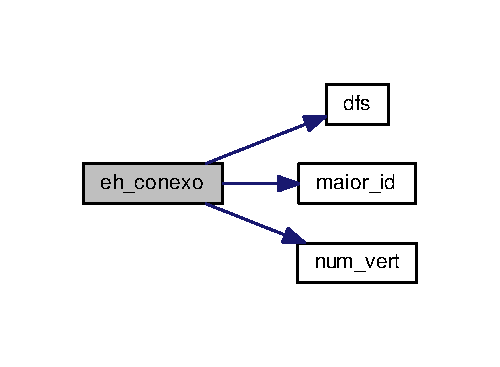
\includegraphics[width=240pt]{grafo_8h_a46f8363c4da6edf056e5fffba46e1bc7_cgraph}
\end{center}
\end{figure}


\hypertarget{grafo_8h_a56edc294bdf9e834989d9c8d31ed3a64}{}\index{grafo.\+h@{grafo.\+h}!existe\+\_\+aresta@{existe\+\_\+aresta}}
\index{existe\+\_\+aresta@{existe\+\_\+aresta}!grafo.\+h@{grafo.\+h}}
\subsubsection[{existe\+\_\+aresta(const grafo\+\_\+priv\+\_\+t $\ast$meu\+\_\+grafo, int id\+\_\+externo1, int id\+\_\+externo2)}]{\setlength{\rightskip}{0pt plus 5cm}{\bf resposta} existe\+\_\+aresta (
\begin{DoxyParamCaption}
\item[{const {\bf grafo\+\_\+priv\+\_\+t} $\ast$}]{meu\+\_\+grafo, }
\item[{int}]{id\+\_\+externo1, }
\item[{int}]{id\+\_\+externo2}
\end{DoxyParamCaption}
)}\label{grafo_8h_a56edc294bdf9e834989d9c8d31ed3a64}


Definição na linha 87 do arquivo grafo.\+cpp.



Referências lista\+\_\+aresta\+::destino, existe\+\_\+vert(), F\+A\+L\+S\+E\+\_\+\+T, lista\+\_\+vert\+::id\+\_\+externo, lista\+\_\+aresta\+::next, lista\+\_\+vert\+::next, lista\+\_\+vert\+::sucessores, T\+R\+U\+E\+\_\+\+T e grafo\+\_\+priv\+::vert.



Referenciado por inserir\+\_\+aresta() e remover\+\_\+aresta().



Este é o diagrama das funções utilizadas por esta função\+:\nopagebreak
\begin{figure}[H]
\begin{center}
\leavevmode
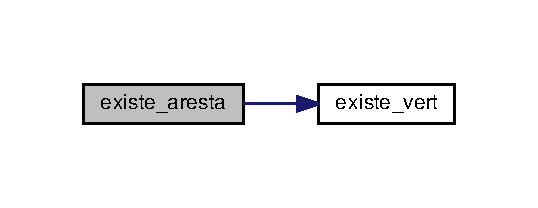
\includegraphics[width=258pt]{grafo_8h_a56edc294bdf9e834989d9c8d31ed3a64_cgraph}
\end{center}
\end{figure}




Este é o diagrama das funções que utilizam esta função\+:
\nopagebreak
\begin{figure}[H]
\begin{center}
\leavevmode
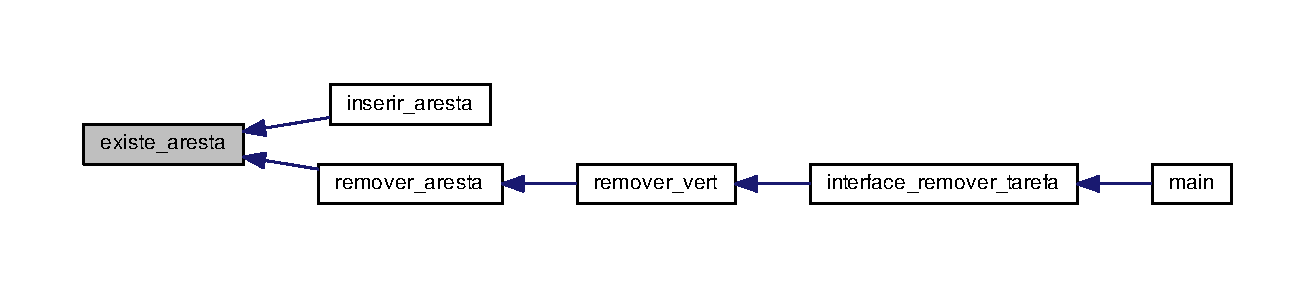
\includegraphics[width=350pt]{grafo_8h_a56edc294bdf9e834989d9c8d31ed3a64_icgraph}
\end{center}
\end{figure}


\hypertarget{grafo_8h_ac70f5a4fd6ff7c6913f0ce99de099263}{}\index{grafo.\+h@{grafo.\+h}!existe\+\_\+vert@{existe\+\_\+vert}}
\index{existe\+\_\+vert@{existe\+\_\+vert}!grafo.\+h@{grafo.\+h}}
\subsubsection[{existe\+\_\+vert(const grafo\+\_\+priv\+\_\+t $\ast$meu\+\_\+grafo, int id\+\_\+externo)}]{\setlength{\rightskip}{0pt plus 5cm}{\bf resposta} existe\+\_\+vert (
\begin{DoxyParamCaption}
\item[{const {\bf grafo\+\_\+priv\+\_\+t} $\ast$}]{meu\+\_\+grafo, }
\item[{int}]{id\+\_\+externo}
\end{DoxyParamCaption}
)}\label{grafo_8h_ac70f5a4fd6ff7c6913f0ce99de099263}


Definição na linha 64 do arquivo grafo.\+cpp.



Referências lista\+\_\+vert\+\_\+codigo\+::dado, F\+A\+L\+S\+E\+\_\+\+T, Celula\+\_\+priv\+::id\+\_\+externo, lista\+\_\+vert\+\_\+codigo\+::next, grafo\+\_\+priv\+::tabela e T\+R\+U\+E\+\_\+\+T.



Referenciado por existe\+\_\+aresta(), existe\+\_\+origem(), inserir\+\_\+aresta(), inserir\+\_\+origem(), inserir\+\_\+vert(), remover\+\_\+aresta(), remover\+\_\+origem() e remover\+\_\+vert().



Este é o diagrama das funções que utilizam esta função\+:
\nopagebreak
\begin{figure}[H]
\begin{center}
\leavevmode
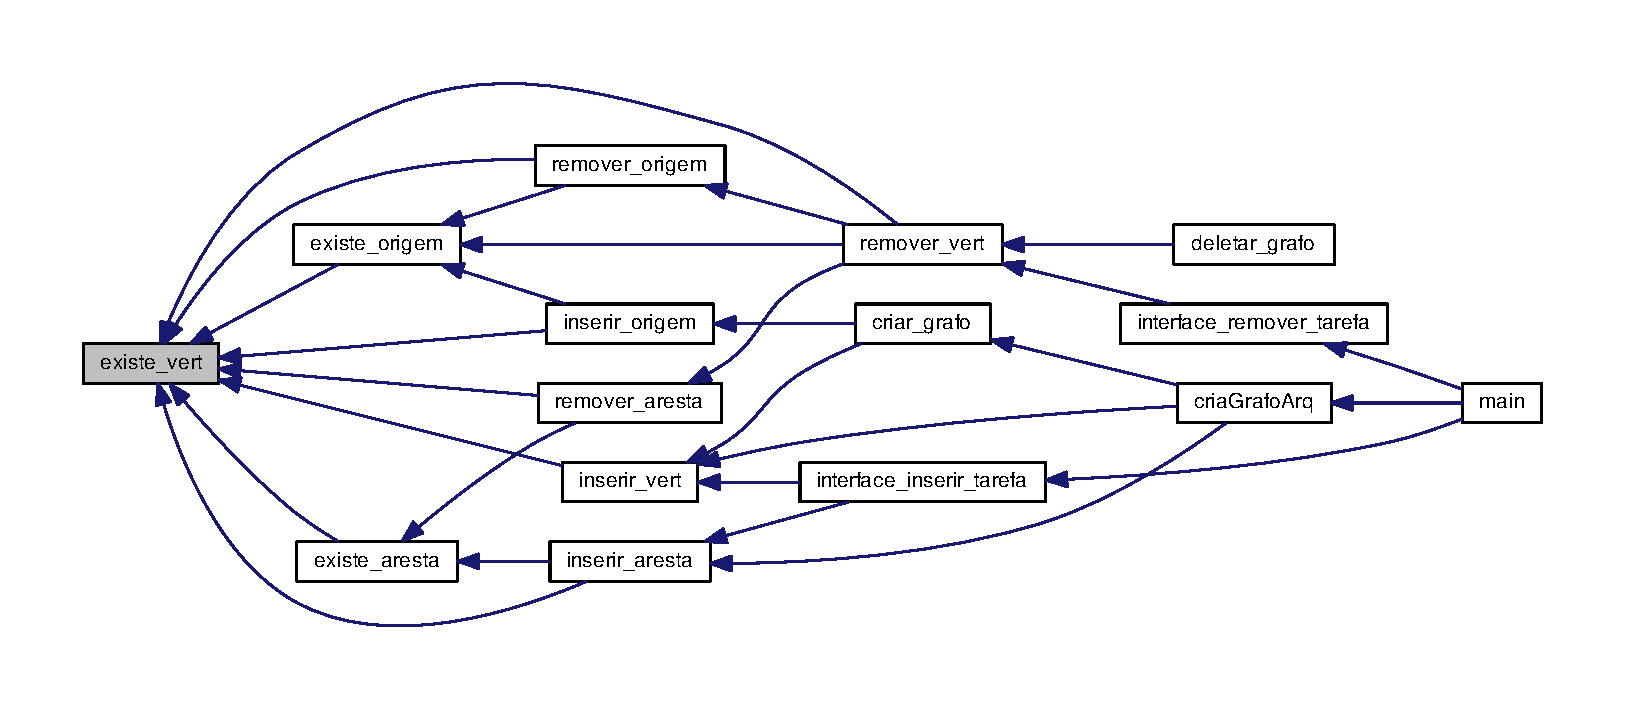
\includegraphics[width=350pt]{grafo_8h_ac70f5a4fd6ff7c6913f0ce99de099263_icgraph}
\end{center}
\end{figure}


\hypertarget{grafo_8h_aadbd57b376954aeeb119120d5a4a196f}{}\index{grafo.\+h@{grafo.\+h}!Grava\+\_\+\+Arq@{Grava\+\_\+\+Arq}}
\index{Grava\+\_\+\+Arq@{Grava\+\_\+\+Arq}!grafo.\+h@{grafo.\+h}}
\subsubsection[{Grava\+\_\+\+Arq(grafo\+\_\+priv\+\_\+t $\ast$meu\+\_\+grafo, char $\ast$\+Nome\+Arq)}]{\setlength{\rightskip}{0pt plus 5cm}void Grava\+\_\+\+Arq (
\begin{DoxyParamCaption}
\item[{{\bf grafo\+\_\+priv\+\_\+t} $\ast$}]{meu\+\_\+grafo, }
\item[{char $\ast$}]{Nome\+Arq}
\end{DoxyParamCaption}
)}\label{grafo_8h_aadbd57b376954aeeb119120d5a4a196f}


Definição na linha 636 do arquivo grafo.\+cpp.



Referências lista\+\_\+vert\+\_\+codigo\+::dado, Celula\+\_\+priv\+::duracao, Celula\+\_\+priv\+::executada, Celula\+\_\+priv\+::id\+\_\+externo, Celula\+\_\+priv\+::ini\+\_\+min, lista\+\_\+vert\+\_\+codigo\+::next, Celula\+\_\+priv\+::nome, Celula\+\_\+priv\+::pre\+\_\+req, Celula\+\_\+priv\+::reqs e grafo\+\_\+priv\+::tabela.



Referenciado por main().



Este é o diagrama das funções que utilizam esta função\+:\nopagebreak
\begin{figure}[H]
\begin{center}
\leavevmode
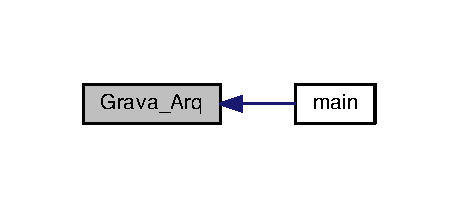
\includegraphics[width=220pt]{grafo_8h_aadbd57b376954aeeb119120d5a4a196f_icgraph}
\end{center}
\end{figure}


\hypertarget{grafo_8h_a1dd7cc6696ade339827db4d2019239fc}{}\index{grafo.\+h@{grafo.\+h}!Imprime\+\_\+\+Tarefas@{Imprime\+\_\+\+Tarefas}}
\index{Imprime\+\_\+\+Tarefas@{Imprime\+\_\+\+Tarefas}!grafo.\+h@{grafo.\+h}}
\subsubsection[{Imprime\+\_\+\+Tarefas(const grafo\+\_\+priv\+\_\+t $\ast$meu\+\_\+grafo, int linha, int coluna)}]{\setlength{\rightskip}{0pt plus 5cm}void Imprime\+\_\+\+Tarefas (
\begin{DoxyParamCaption}
\item[{const {\bf grafo\+\_\+priv\+\_\+t} $\ast$}]{meu\+\_\+grafo, }
\item[{int}]{linha, }
\item[{int}]{coluna}
\end{DoxyParamCaption}
)}\label{grafo_8h_a1dd7cc6696ade339827db4d2019239fc}


Definição na linha 616 do arquivo grafo.\+cpp.



Referências lista\+\_\+vert\+\_\+codigo\+::dado, Celula\+\_\+priv\+::duracao, Celula\+\_\+priv\+::executada, Celula\+\_\+priv\+::id\+\_\+externo, Celula\+\_\+priv\+::ini\+\_\+min, lista\+\_\+vert\+\_\+codigo\+::next, Celula\+\_\+priv\+::nome, Celula\+\_\+priv\+::pre\+\_\+req, Celula\+\_\+priv\+::reqs e grafo\+\_\+priv\+::tabela.



Referenciado por interface\+\_\+vizualizar\+\_\+tarefas().



Este é o diagrama das funções que utilizam esta função\+:\nopagebreak
\begin{figure}[H]
\begin{center}
\leavevmode
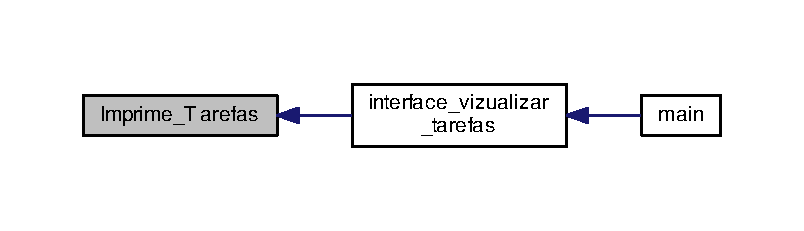
\includegraphics[width=350pt]{grafo_8h_a1dd7cc6696ade339827db4d2019239fc_icgraph}
\end{center}
\end{figure}


\hypertarget{grafo_8h_a0e69707897c891bf77319d494cae8f26}{}\index{grafo.\+h@{grafo.\+h}!inserir\+\_\+aresta@{inserir\+\_\+aresta}}
\index{inserir\+\_\+aresta@{inserir\+\_\+aresta}!grafo.\+h@{grafo.\+h}}
\subsubsection[{inserir\+\_\+aresta(grafo\+\_\+priv\+\_\+t $\ast$meu\+\_\+grafo, int id\+\_\+externo1, Celula\+\_\+priv\+\_\+t $\ast$celula2, int peso)}]{\setlength{\rightskip}{0pt plus 5cm}void inserir\+\_\+aresta (
\begin{DoxyParamCaption}
\item[{{\bf grafo\+\_\+priv\+\_\+t} $\ast$}]{meu\+\_\+grafo, }
\item[{int}]{id\+\_\+externo1, }
\item[{{\bf Celula\+\_\+priv\+\_\+t} $\ast$}]{celula2, }
\item[{int}]{peso}
\end{DoxyParamCaption}
)}\label{grafo_8h_a0e69707897c891bf77319d494cae8f26}


Definição na linha 250 do arquivo grafo.\+cpp.



Referências achar\+\_\+id(), lista\+\_\+aresta\+::destino, existe\+\_\+aresta(), existe\+\_\+vert(), F\+A\+L\+S\+E\+\_\+\+T, Celula\+\_\+priv\+::id\+\_\+externo, lista\+\_\+aresta\+::next, lista\+\_\+vert\+::next, Celula\+\_\+priv\+::nome, lista\+\_\+aresta\+::peso, lista\+\_\+vert\+::sucessores, T\+R\+U\+E\+\_\+\+T e grafo\+\_\+priv\+::vert.



Referenciado por cria\+Grafo\+Arq() e interface\+\_\+inserir\+\_\+tarefa().



Este é o diagrama das funções utilizadas por esta função\+:\nopagebreak
\begin{figure}[H]
\begin{center}
\leavevmode
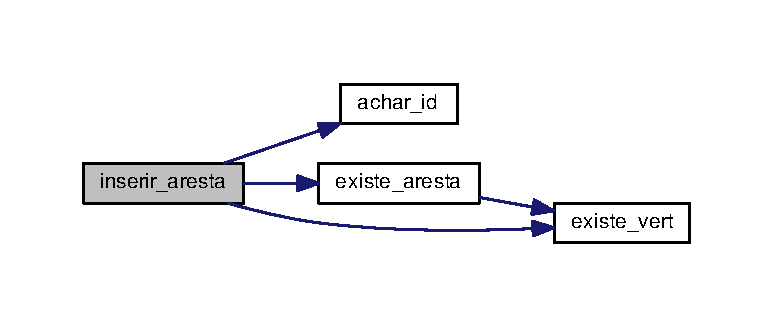
\includegraphics[width=350pt]{grafo_8h_a0e69707897c891bf77319d494cae8f26_cgraph}
\end{center}
\end{figure}




Este é o diagrama das funções que utilizam esta função\+:\nopagebreak
\begin{figure}[H]
\begin{center}
\leavevmode
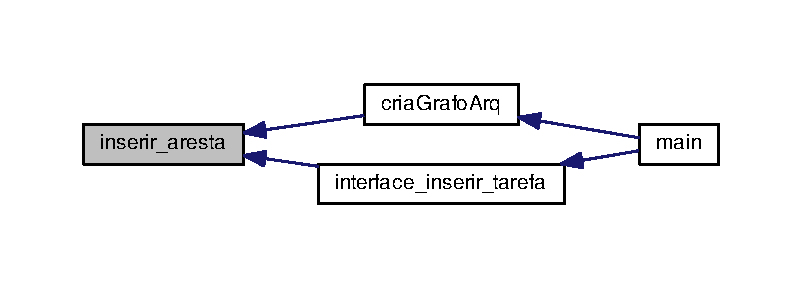
\includegraphics[width=350pt]{grafo_8h_a0e69707897c891bf77319d494cae8f26_icgraph}
\end{center}
\end{figure}


\hypertarget{grafo_8h_a659b567cb7e165b526b6fe05a433452e}{}\index{grafo.\+h@{grafo.\+h}!inserir\+\_\+vert@{inserir\+\_\+vert}}
\index{inserir\+\_\+vert@{inserir\+\_\+vert}!grafo.\+h@{grafo.\+h}}
\subsubsection[{inserir\+\_\+vert(grafo\+\_\+priv\+\_\+t $\ast$meu\+\_\+grafo, Celula\+\_\+priv\+\_\+t $\ast$celula)}]{\setlength{\rightskip}{0pt plus 5cm}void inserir\+\_\+vert (
\begin{DoxyParamCaption}
\item[{{\bf grafo\+\_\+priv\+\_\+t} $\ast$}]{meu\+\_\+grafo, }
\item[{{\bf Celula\+\_\+priv\+\_\+t} $\ast$}]{celula}
\end{DoxyParamCaption}
)}\label{grafo_8h_a659b567cb7e165b526b6fe05a433452e}


Definição na linha 128 do arquivo grafo.\+cpp.



Referências lista\+\_\+vert\+::antecessores, existe\+\_\+vert(), F\+A\+L\+S\+E\+\_\+\+T, lista\+\_\+vert\+\_\+codigo\+::id, lista\+\_\+vert\+::id, Celula\+\_\+priv\+::id\+\_\+externo, lista\+\_\+vert\+::id\+\_\+externo, Celula\+\_\+priv\+::ini\+\_\+min, lista\+\_\+vert\+\_\+codigo\+::next, lista\+\_\+vert\+::next, Celula\+\_\+priv\+::nome, Celula\+\_\+priv\+::pre\+\_\+req, lista\+\_\+vert\+::sucessores, grafo\+\_\+priv\+::tabela e grafo\+\_\+priv\+::vert.



Referenciado por cria\+Grafo\+Arq(), criar\+\_\+grafo() e interface\+\_\+inserir\+\_\+tarefa().



Este é o diagrama das funções utilizadas por esta função\+:\nopagebreak
\begin{figure}[H]
\begin{center}
\leavevmode
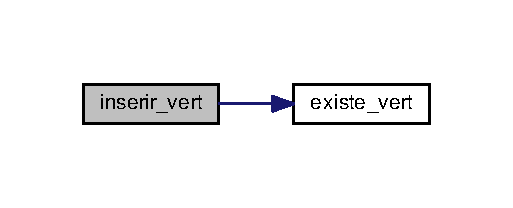
\includegraphics[width=246pt]{grafo_8h_a659b567cb7e165b526b6fe05a433452e_cgraph}
\end{center}
\end{figure}




Este é o diagrama das funções que utilizam esta função\+:\nopagebreak
\begin{figure}[H]
\begin{center}
\leavevmode
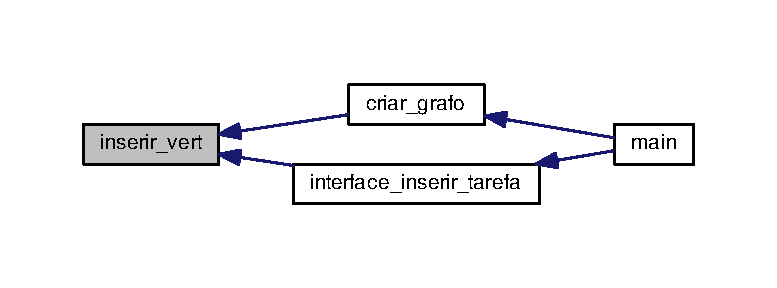
\includegraphics[width=350pt]{grafo_8h_a659b567cb7e165b526b6fe05a433452e_icgraph}
\end{center}
\end{figure}


\hypertarget{grafo_8h_acb5b55f7d1508a1b35b76e43bc817623}{}\index{grafo.\+h@{grafo.\+h}!ja\+\_\+feito@{ja\+\_\+feito}}
\index{ja\+\_\+feito@{ja\+\_\+feito}!grafo.\+h@{grafo.\+h}}
\subsubsection[{ja\+\_\+feito(const grafo\+\_\+priv\+\_\+t $\ast$meu\+\_\+grafo, int d)}]{\setlength{\rightskip}{0pt plus 5cm}void ja\+\_\+feito (
\begin{DoxyParamCaption}
\item[{const {\bf grafo\+\_\+priv\+\_\+t} $\ast$}]{meu\+\_\+grafo, }
\item[{int}]{d}
\end{DoxyParamCaption}
)}\label{grafo_8h_acb5b55f7d1508a1b35b76e43bc817623}


Definição na linha 733 do arquivo grafo.\+cpp.



Referências lista\+\_\+vert\+\_\+codigo\+::id, menor\+\_\+caminho(), lista\+\_\+vert\+\_\+codigo\+::next e grafo\+\_\+priv\+::tabela.



Este é o diagrama das funções utilizadas por esta função\+:\nopagebreak
\begin{figure}[H]
\begin{center}
\leavevmode
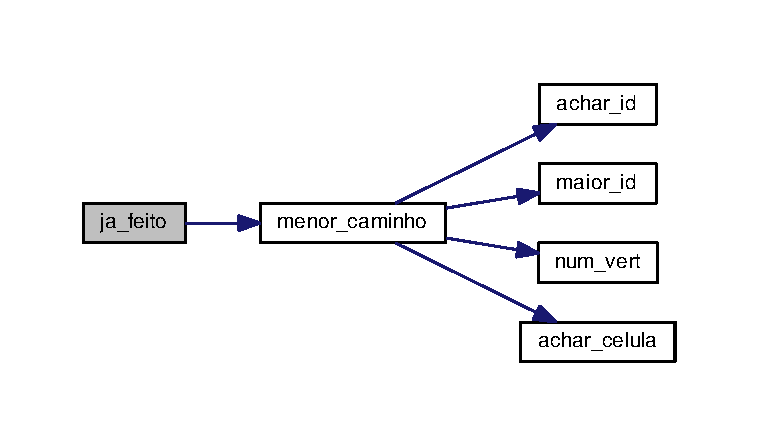
\includegraphics[width=350pt]{grafo_8h_acb5b55f7d1508a1b35b76e43bc817623_cgraph}
\end{center}
\end{figure}


\hypertarget{grafo_8h_acd0aa806c04807a2b8086bd7a6c59b50}{}\index{grafo.\+h@{grafo.\+h}!Ler\+\_\+\+Tarefas@{Ler\+\_\+\+Tarefas}}
\index{Ler\+\_\+\+Tarefas@{Ler\+\_\+\+Tarefas}!grafo.\+h@{grafo.\+h}}
\subsubsection[{Ler\+\_\+\+Tarefas(grafo\+\_\+priv\+\_\+t $\ast$meu\+\_\+grafo, Celula\+\_\+priv\+\_\+t $\ast$celula, const char $\ast$\+Nome\+Arq)}]{\setlength{\rightskip}{0pt plus 5cm}void Ler\+\_\+\+Tarefas (
\begin{DoxyParamCaption}
\item[{{\bf grafo\+\_\+priv\+\_\+t} $\ast$}]{meu\+\_\+grafo, }
\item[{{\bf Celula\+\_\+priv\+\_\+t} $\ast$}]{celula, }
\item[{const char $\ast$}]{Nome\+Arq}
\end{DoxyParamCaption}
)}\label{grafo_8h_acd0aa806c04807a2b8086bd7a6c59b50}
\hypertarget{grafo_8h_a5bedfb800e326da354b0403421e0d1ef}{}\index{grafo.\+h@{grafo.\+h}!maior\+\_\+id@{maior\+\_\+id}}
\index{maior\+\_\+id@{maior\+\_\+id}!grafo.\+h@{grafo.\+h}}
\subsubsection[{maior\+\_\+id(const grafo\+\_\+priv\+\_\+t $\ast$meu\+\_\+grafo)}]{\setlength{\rightskip}{0pt plus 5cm}int maior\+\_\+id (
\begin{DoxyParamCaption}
\item[{const {\bf grafo\+\_\+priv\+\_\+t} $\ast$}]{meu\+\_\+grafo}
\end{DoxyParamCaption}
)}\label{grafo_8h_a5bedfb800e326da354b0403421e0d1ef}


Definição na linha 490 do arquivo grafo.\+cpp.



Referências lista\+\_\+vert\+\_\+codigo\+::id, lista\+\_\+vert\+\_\+codigo\+::next e grafo\+\_\+priv\+::tabela.



Referenciado por eh\+\_\+conexo() e menor\+\_\+caminho().



Este é o diagrama das funções que utilizam esta função\+:\nopagebreak
\begin{figure}[H]
\begin{center}
\leavevmode
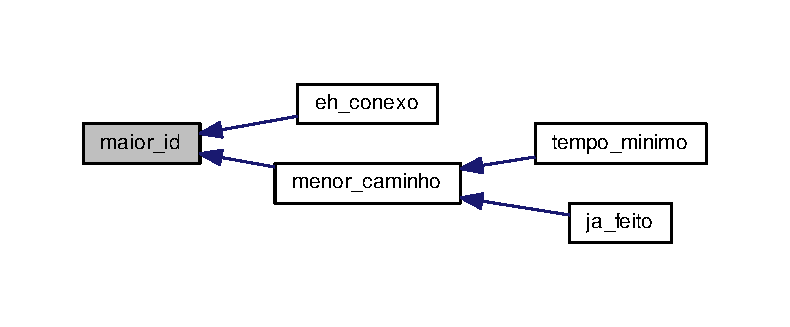
\includegraphics[width=350pt]{grafo_8h_a5bedfb800e326da354b0403421e0d1ef_icgraph}
\end{center}
\end{figure}


\hypertarget{grafo_8h_ad507a38f9feef6cad69436ec774b535f}{}\index{grafo.\+h@{grafo.\+h}!menor\+\_\+caminho@{menor\+\_\+caminho}}
\index{menor\+\_\+caminho@{menor\+\_\+caminho}!grafo.\+h@{grafo.\+h}}
\subsubsection[{menor\+\_\+caminho(const grafo\+\_\+priv\+\_\+t $\ast$meu\+\_\+grafo, int $\ast$$\ast$dist)}]{\setlength{\rightskip}{0pt plus 5cm}int menor\+\_\+caminho (
\begin{DoxyParamCaption}
\item[{const {\bf grafo\+\_\+priv\+\_\+t} $\ast$}]{meu\+\_\+grafo, }
\item[{int $\ast$$\ast$}]{dist}
\end{DoxyParamCaption}
)}\label{grafo_8h_ad507a38f9feef6cad69436ec774b535f}


Definição na linha 524 do arquivo grafo.\+cpp.



Referências achar\+\_\+celula(), achar\+\_\+id(), lista\+\_\+aresta\+::destino, lista\+\_\+vert\+::id, Celula\+\_\+priv\+::ini\+\_\+min, maior\+\_\+id(), lista\+\_\+aresta\+::next, lista\+\_\+vert\+::next, num\+\_\+vert(), lista\+\_\+aresta\+::peso, lista\+\_\+vert\+::sucessores e grafo\+\_\+priv\+::vert.



Referenciado por ja\+\_\+feito() e tempo\+\_\+minimo().



Este é o diagrama das funções utilizadas por esta função\+:\nopagebreak
\begin{figure}[H]
\begin{center}
\leavevmode
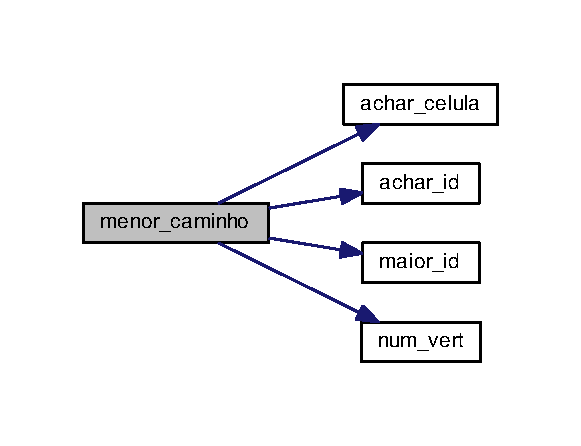
\includegraphics[width=279pt]{grafo_8h_ad507a38f9feef6cad69436ec774b535f_cgraph}
\end{center}
\end{figure}




Este é o diagrama das funções que utilizam esta função\+:\nopagebreak
\begin{figure}[H]
\begin{center}
\leavevmode
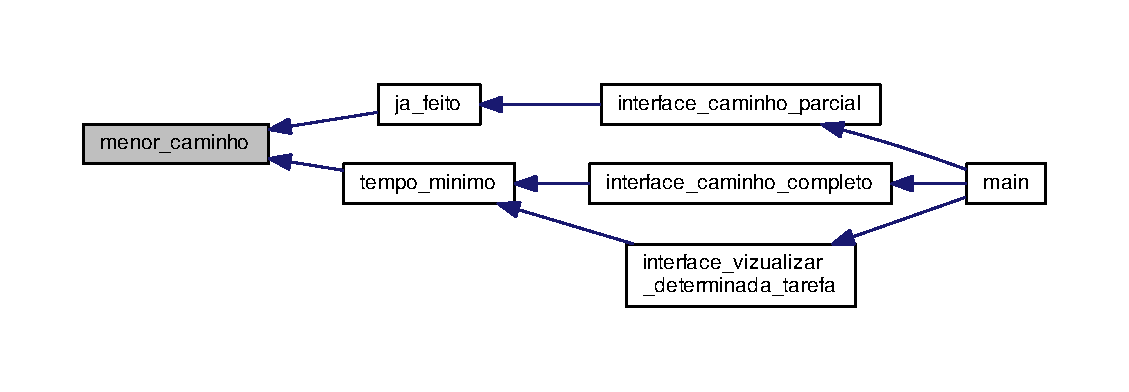
\includegraphics[width=287pt]{grafo_8h_ad507a38f9feef6cad69436ec774b535f_icgraph}
\end{center}
\end{figure}


\hypertarget{grafo_8h_ac94be03e94792b9b868abb38c7e17e36}{}\index{grafo.\+h@{grafo.\+h}!num\+\_\+arestas@{num\+\_\+arestas}}
\index{num\+\_\+arestas@{num\+\_\+arestas}!grafo.\+h@{grafo.\+h}}
\subsubsection[{num\+\_\+arestas(const grafo\+\_\+priv\+\_\+t $\ast$meu\+\_\+grafo)}]{\setlength{\rightskip}{0pt plus 5cm}int num\+\_\+arestas (
\begin{DoxyParamCaption}
\item[{const {\bf grafo\+\_\+priv\+\_\+t} $\ast$}]{meu\+\_\+grafo}
\end{DoxyParamCaption}
)}\label{grafo_8h_ac94be03e94792b9b868abb38c7e17e36}


Definição na linha 511 do arquivo grafo.\+cpp.



Referências lista\+\_\+aresta\+::next, lista\+\_\+vert\+::next, lista\+\_\+vert\+::sucessores e grafo\+\_\+priv\+::vert.

\hypertarget{grafo_8h_a31c64875fe3134ba04439feb7d119cf3}{}\index{grafo.\+h@{grafo.\+h}!num\+\_\+vert@{num\+\_\+vert}}
\index{num\+\_\+vert@{num\+\_\+vert}!grafo.\+h@{grafo.\+h}}
\subsubsection[{num\+\_\+vert(const grafo\+\_\+priv\+\_\+t $\ast$meu\+\_\+grafo)}]{\setlength{\rightskip}{0pt plus 5cm}int num\+\_\+vert (
\begin{DoxyParamCaption}
\item[{const {\bf grafo\+\_\+priv\+\_\+t} $\ast$}]{meu\+\_\+grafo}
\end{DoxyParamCaption}
)}\label{grafo_8h_a31c64875fe3134ba04439feb7d119cf3}


Definição na linha 501 do arquivo grafo.\+cpp.



Referências lista\+\_\+vert\+::next e grafo\+\_\+priv\+::vert.



Referenciado por eh\+\_\+conexo() e menor\+\_\+caminho().



Este é o diagrama das funções que utilizam esta função\+:\nopagebreak
\begin{figure}[H]
\begin{center}
\leavevmode
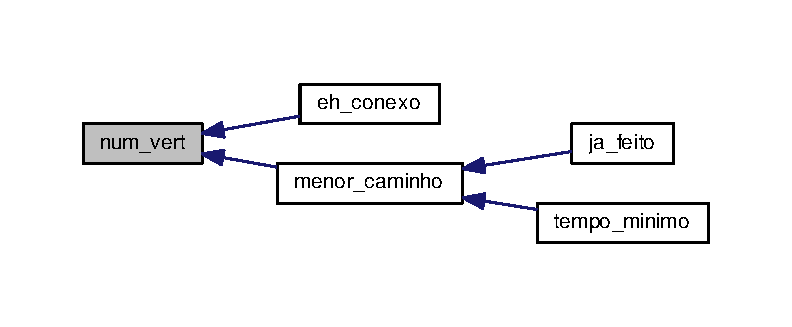
\includegraphics[width=350pt]{grafo_8h_a31c64875fe3134ba04439feb7d119cf3_icgraph}
\end{center}
\end{figure}


\hypertarget{grafo_8h_ac16199e4256247b546b67d6d881be137}{}\index{grafo.\+h@{grafo.\+h}!remover\+\_\+aresta@{remover\+\_\+aresta}}
\index{remover\+\_\+aresta@{remover\+\_\+aresta}!grafo.\+h@{grafo.\+h}}
\subsubsection[{remover\+\_\+aresta(grafo\+\_\+priv\+\_\+t $\ast$meu\+\_\+grafo, int id\+\_\+externo1, int id\+\_\+externo2)}]{\setlength{\rightskip}{0pt plus 5cm}void remover\+\_\+aresta (
\begin{DoxyParamCaption}
\item[{{\bf grafo\+\_\+priv\+\_\+t} $\ast$}]{meu\+\_\+grafo, }
\item[{int}]{id\+\_\+externo1, }
\item[{int}]{id\+\_\+externo2}
\end{DoxyParamCaption}
)}\label{grafo_8h_ac16199e4256247b546b67d6d881be137}


Definição na linha 440 do arquivo grafo.\+cpp.



Referências achar\+\_\+id(), lista\+\_\+vert\+::antecessores, existe\+\_\+aresta(), existe\+\_\+vert(), lista\+\_\+vert\+::id, lista\+\_\+aresta\+::next, lista\+\_\+vert\+::next, lista\+\_\+vert\+::sucessores, T\+R\+U\+E\+\_\+\+T e grafo\+\_\+priv\+::vert.



Referenciado por remover\+\_\+vert().



Este é o diagrama das funções utilizadas por esta função\+:\nopagebreak
\begin{figure}[H]
\begin{center}
\leavevmode
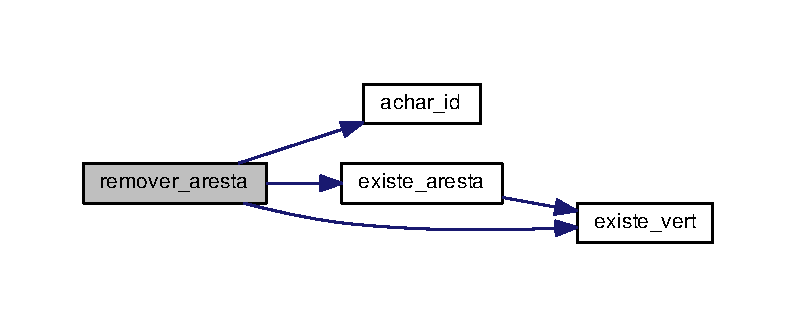
\includegraphics[width=350pt]{grafo_8h_ac16199e4256247b546b67d6d881be137_cgraph}
\end{center}
\end{figure}




Este é o diagrama das funções que utilizam esta função\+:
\nopagebreak
\begin{figure}[H]
\begin{center}
\leavevmode
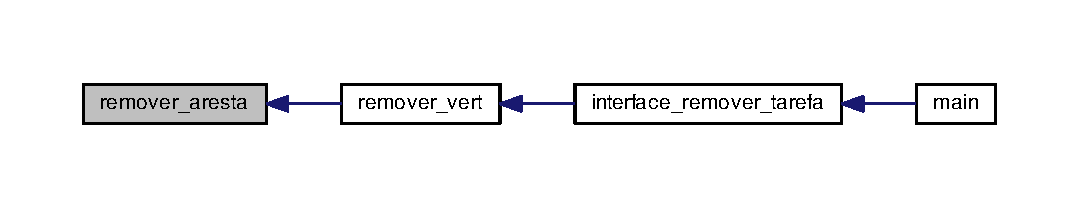
\includegraphics[width=350pt]{grafo_8h_ac16199e4256247b546b67d6d881be137_icgraph}
\end{center}
\end{figure}


\hypertarget{grafo_8h_a2812c8a1cbeaab16d0aaa6da10ec4372}{}\index{grafo.\+h@{grafo.\+h}!remover\+\_\+vert@{remover\+\_\+vert}}
\index{remover\+\_\+vert@{remover\+\_\+vert}!grafo.\+h@{grafo.\+h}}
\subsubsection[{remover\+\_\+vert(grafo\+\_\+priv\+\_\+t $\ast$meu\+\_\+grafo, int id\+\_\+externo)}]{\setlength{\rightskip}{0pt plus 5cm}void remover\+\_\+vert (
\begin{DoxyParamCaption}
\item[{{\bf grafo\+\_\+priv\+\_\+t} $\ast$}]{meu\+\_\+grafo, }
\item[{int}]{id\+\_\+externo}
\end{DoxyParamCaption}
)}\label{grafo_8h_a2812c8a1cbeaab16d0aaa6da10ec4372}


Definição na linha 340 do arquivo grafo.\+cpp.



Referências achar\+\_\+id(), lista\+\_\+aresta\+::destino, existe\+\_\+origem(), existe\+\_\+vert(), lista\+\_\+vert\+\_\+codigo\+::id, lista\+\_\+vert\+::id, lista\+\_\+vert\+::id\+\_\+externo, lista\+\_\+vert\+\_\+codigo\+::next, lista\+\_\+vert\+::next, remover\+\_\+aresta(), remover\+\_\+origem(), grafo\+\_\+priv\+::tabela, T\+R\+U\+E\+\_\+\+T e grafo\+\_\+priv\+::vert.



Referenciado por deletar\+\_\+grafo() e interface\+\_\+remover\+\_\+tarefa().



Este é o diagrama das funções utilizadas por esta função\+:\nopagebreak
\begin{figure}[H]
\begin{center}
\leavevmode
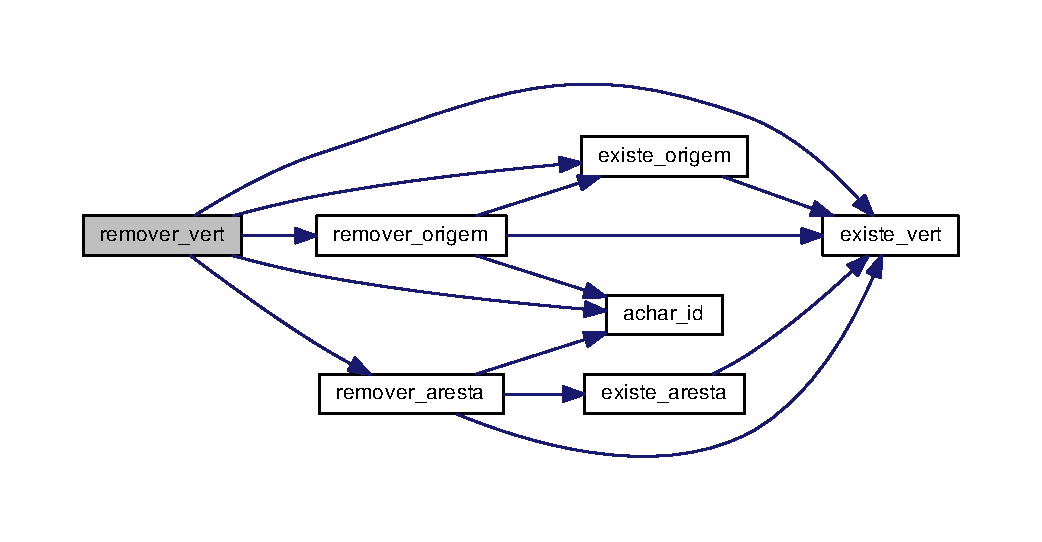
\includegraphics[width=350pt]{grafo_8h_a2812c8a1cbeaab16d0aaa6da10ec4372_cgraph}
\end{center}
\end{figure}




Este é o diagrama das funções que utilizam esta função\+:
\nopagebreak
\begin{figure}[H]
\begin{center}
\leavevmode
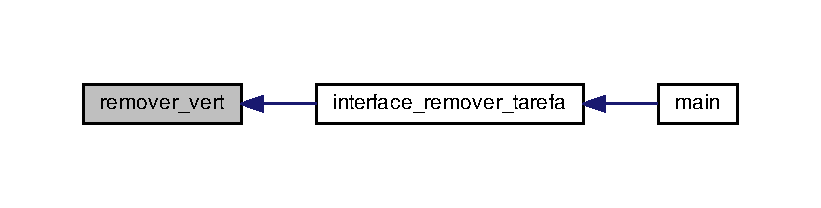
\includegraphics[width=350pt]{grafo_8h_a2812c8a1cbeaab16d0aaa6da10ec4372_icgraph}
\end{center}
\end{figure}


\hypertarget{grafo_8h_a14183876086781302e2d81ab2457dc4e}{}\index{grafo.\+h@{grafo.\+h}!tempo\+\_\+minimo@{tempo\+\_\+minimo}}
\index{tempo\+\_\+minimo@{tempo\+\_\+minimo}!grafo.\+h@{grafo.\+h}}
\subsubsection[{tempo\+\_\+minimo(const grafo\+\_\+priv\+\_\+t $\ast$meu\+\_\+grafo, int id\+\_\+fim)}]{\setlength{\rightskip}{0pt plus 5cm}int tempo\+\_\+minimo (
\begin{DoxyParamCaption}
\item[{const {\bf grafo\+\_\+priv\+\_\+t} $\ast$}]{meu\+\_\+grafo, }
\item[{int}]{id\+\_\+fim}
\end{DoxyParamCaption}
)}\label{grafo_8h_a14183876086781302e2d81ab2457dc4e}


Definição na linha 718 do arquivo grafo.\+cpp.



Referências menor\+\_\+caminho().



Este é o diagrama das funções utilizadas por esta função\+:\nopagebreak
\begin{figure}[H]
\begin{center}
\leavevmode
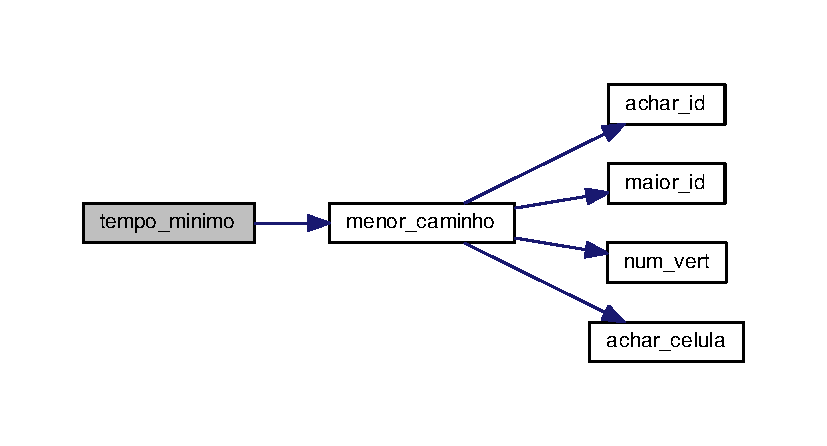
\includegraphics[width=350pt]{grafo_8h_a14183876086781302e2d81ab2457dc4e_cgraph}
\end{center}
\end{figure}



\hypertarget{grafo__priv_8h}{}\section{Referência do Arquivo /home/rafael/\+Projeto\+Final\+M\+P/\+Fase2\+Interface/include/grafo\+\_\+priv.h}
\label{grafo__priv_8h}\index{/home/rafael/\+Projeto\+Final\+M\+P/\+Fase2\+Interface/include/grafo\+\_\+priv.\+h@{/home/rafael/\+Projeto\+Final\+M\+P/\+Fase2\+Interface/include/grafo\+\_\+priv.\+h}}
{\ttfamily \#include \char`\"{}grafo.\+h\char`\"{}}\\*
Gráfico de dependência de inclusões para grafo\+\_\+priv.\+h\+:
\nopagebreak
\begin{figure}[H]
\begin{center}
\leavevmode
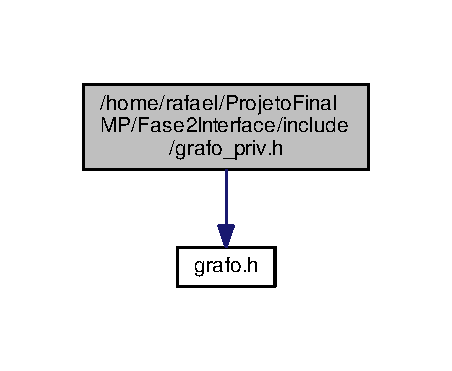
\includegraphics[width=217pt]{grafo__priv_8h__incl}
\end{center}
\end{figure}
Este grafo mostra quais arquivos estão direta ou indiretamente relacionados com este arquivo\+:
\nopagebreak
\begin{figure}[H]
\begin{center}
\leavevmode
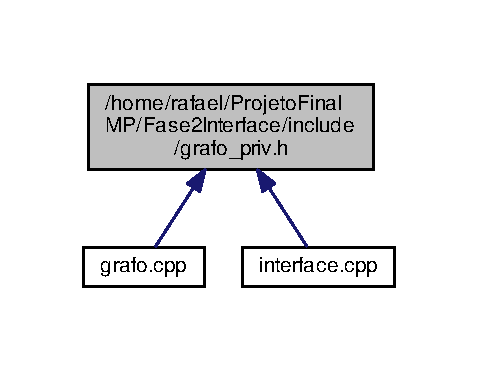
\includegraphics[width=230pt]{grafo__priv_8h__dep__incl}
\end{center}
\end{figure}
\subsection*{Estruturas de Dados}
\begin{DoxyCompactItemize}
\item 
struct \hyperlink{structCelula__priv}{Celula\+\_\+priv}
\item 
struct \hyperlink{structlista__vert__codigo}{lista\+\_\+vert\+\_\+codigo}
\item 
struct \hyperlink{structlista__aresta}{lista\+\_\+aresta}
\item 
struct \hyperlink{structlista__vert}{lista\+\_\+vert}
\item 
struct \hyperlink{structlista__origem}{lista\+\_\+origem}
\item 
struct \hyperlink{structgrafo__priv}{grafo\+\_\+priv}
\end{DoxyCompactItemize}
\subsection*{Definições de Tipos}
\begin{DoxyCompactItemize}
\item 
typedef struct \hyperlink{structCelula__priv}{Celula\+\_\+priv} \hyperlink{grafo__priv_8h_a54889edec2a20c11a5015e4437a6b656}{Celula\+\_\+priv\+\_\+t}
\item 
typedef struct \hyperlink{structlista__vert__codigo}{lista\+\_\+vert\+\_\+codigo} \hyperlink{grafo__priv_8h_ae17c76eddcd8bd44e7d91faf7c00e2e5}{lista\+\_\+vert\+\_\+codigo\+\_\+t}
\item 
typedef struct \hyperlink{structlista__aresta}{lista\+\_\+aresta} \hyperlink{grafo__priv_8h_a8c99b03365ae7f753c4cf1a20d9e9257}{lista\+\_\+aresta\+\_\+t}
\item 
typedef struct \hyperlink{structlista__vert}{lista\+\_\+vert} \hyperlink{grafo__priv_8h_aecb68281fecb412bf6427dd6a07d5077}{lista\+\_\+vert\+\_\+t}
\item 
typedef struct \hyperlink{structlista__origem}{lista\+\_\+origem} \hyperlink{grafo__priv_8h_a91c8b187403e9724a757c92c941ab631}{lista\+\_\+origem\+\_\+t}
\item 
typedef struct \hyperlink{structgrafo__priv}{grafo\+\_\+priv} \hyperlink{grafo__priv_8h_a35fb938b8d010a769f7317ea5d8cb237}{grafo\+\_\+priv\+\_\+t}
\end{DoxyCompactItemize}
\subsection*{Funções}
\begin{DoxyCompactItemize}
\item 
\hyperlink{grafo_8h_a64f906a639abdfda7fffa9ace7e4c286}{resposta} \hyperlink{grafo__priv_8h_aa7c7803e91592a28e4c0a85112b53fb8}{existe\+\_\+origem} (const \hyperlink{grafo_8h_a282167c584dceb79dde5c159a85b685b}{grafo\+\_\+priv\+\_\+t} $\ast$meu\+\_\+grafo, int id\+\_\+externo)
\item 
void \hyperlink{grafo__priv_8h_adc1a8c08d13a78eda202bc49275712f5}{inserir\+\_\+origem} (\hyperlink{grafo_8h_a282167c584dceb79dde5c159a85b685b}{grafo\+\_\+priv\+\_\+t} $\ast$meu\+\_\+grafo, \hyperlink{grafo_8h_ac2219b5d1f94e440b5895ce440ab23b9}{Celula\+\_\+priv\+\_\+t} $\ast$celula)
\item 
void \hyperlink{grafo__priv_8h_a2f6600bf1f6ecc3c960e244f3e7b5c8f}{remover\+\_\+origem} (\hyperlink{grafo_8h_a282167c584dceb79dde5c159a85b685b}{grafo\+\_\+priv\+\_\+t} $\ast$meu\+\_\+grafo, int id\+\_\+externo)
\end{DoxyCompactItemize}


\subsection{Definições dos tipos}
\hypertarget{grafo__priv_8h_a54889edec2a20c11a5015e4437a6b656}{}\index{grafo\+\_\+priv.\+h@{grafo\+\_\+priv.\+h}!Celula\+\_\+priv\+\_\+t@{Celula\+\_\+priv\+\_\+t}}
\index{Celula\+\_\+priv\+\_\+t@{Celula\+\_\+priv\+\_\+t}!grafo\+\_\+priv.\+h@{grafo\+\_\+priv.\+h}}
\subsubsection[{Celula\+\_\+priv\+\_\+t}]{\setlength{\rightskip}{0pt plus 5cm}typedef struct {\bf Celula\+\_\+priv}  {\bf Celula\+\_\+priv\+\_\+t}}\label{grafo__priv_8h_a54889edec2a20c11a5015e4437a6b656}
\hypertarget{grafo__priv_8h_a35fb938b8d010a769f7317ea5d8cb237}{}\index{grafo\+\_\+priv.\+h@{grafo\+\_\+priv.\+h}!grafo\+\_\+priv\+\_\+t@{grafo\+\_\+priv\+\_\+t}}
\index{grafo\+\_\+priv\+\_\+t@{grafo\+\_\+priv\+\_\+t}!grafo\+\_\+priv.\+h@{grafo\+\_\+priv.\+h}}
\subsubsection[{grafo\+\_\+priv\+\_\+t}]{\setlength{\rightskip}{0pt plus 5cm}typedef struct {\bf grafo\+\_\+priv}  {\bf grafo\+\_\+priv\+\_\+t}}\label{grafo__priv_8h_a35fb938b8d010a769f7317ea5d8cb237}
\hypertarget{grafo__priv_8h_a8c99b03365ae7f753c4cf1a20d9e9257}{}\index{grafo\+\_\+priv.\+h@{grafo\+\_\+priv.\+h}!lista\+\_\+aresta\+\_\+t@{lista\+\_\+aresta\+\_\+t}}
\index{lista\+\_\+aresta\+\_\+t@{lista\+\_\+aresta\+\_\+t}!grafo\+\_\+priv.\+h@{grafo\+\_\+priv.\+h}}
\subsubsection[{lista\+\_\+aresta\+\_\+t}]{\setlength{\rightskip}{0pt plus 5cm}typedef struct {\bf lista\+\_\+aresta}  {\bf lista\+\_\+aresta\+\_\+t}}\label{grafo__priv_8h_a8c99b03365ae7f753c4cf1a20d9e9257}
\hypertarget{grafo__priv_8h_a91c8b187403e9724a757c92c941ab631}{}\index{grafo\+\_\+priv.\+h@{grafo\+\_\+priv.\+h}!lista\+\_\+origem\+\_\+t@{lista\+\_\+origem\+\_\+t}}
\index{lista\+\_\+origem\+\_\+t@{lista\+\_\+origem\+\_\+t}!grafo\+\_\+priv.\+h@{grafo\+\_\+priv.\+h}}
\subsubsection[{lista\+\_\+origem\+\_\+t}]{\setlength{\rightskip}{0pt plus 5cm}typedef struct {\bf lista\+\_\+origem}  {\bf lista\+\_\+origem\+\_\+t}}\label{grafo__priv_8h_a91c8b187403e9724a757c92c941ab631}
\hypertarget{grafo__priv_8h_ae17c76eddcd8bd44e7d91faf7c00e2e5}{}\index{grafo\+\_\+priv.\+h@{grafo\+\_\+priv.\+h}!lista\+\_\+vert\+\_\+codigo\+\_\+t@{lista\+\_\+vert\+\_\+codigo\+\_\+t}}
\index{lista\+\_\+vert\+\_\+codigo\+\_\+t@{lista\+\_\+vert\+\_\+codigo\+\_\+t}!grafo\+\_\+priv.\+h@{grafo\+\_\+priv.\+h}}
\subsubsection[{lista\+\_\+vert\+\_\+codigo\+\_\+t}]{\setlength{\rightskip}{0pt plus 5cm}typedef struct {\bf lista\+\_\+vert\+\_\+codigo}  {\bf lista\+\_\+vert\+\_\+codigo\+\_\+t}}\label{grafo__priv_8h_ae17c76eddcd8bd44e7d91faf7c00e2e5}
\hypertarget{grafo__priv_8h_aecb68281fecb412bf6427dd6a07d5077}{}\index{grafo\+\_\+priv.\+h@{grafo\+\_\+priv.\+h}!lista\+\_\+vert\+\_\+t@{lista\+\_\+vert\+\_\+t}}
\index{lista\+\_\+vert\+\_\+t@{lista\+\_\+vert\+\_\+t}!grafo\+\_\+priv.\+h@{grafo\+\_\+priv.\+h}}
\subsubsection[{lista\+\_\+vert\+\_\+t}]{\setlength{\rightskip}{0pt plus 5cm}typedef struct {\bf lista\+\_\+vert}  {\bf lista\+\_\+vert\+\_\+t}}\label{grafo__priv_8h_aecb68281fecb412bf6427dd6a07d5077}


\subsection{Funções}
\hypertarget{grafo__priv_8h_aa7c7803e91592a28e4c0a85112b53fb8}{}\index{grafo\+\_\+priv.\+h@{grafo\+\_\+priv.\+h}!existe\+\_\+origem@{existe\+\_\+origem}}
\index{existe\+\_\+origem@{existe\+\_\+origem}!grafo\+\_\+priv.\+h@{grafo\+\_\+priv.\+h}}
\subsubsection[{existe\+\_\+origem(const grafo\+\_\+priv\+\_\+t $\ast$meu\+\_\+grafo, int id\+\_\+externo)}]{\setlength{\rightskip}{0pt plus 5cm}{\bf resposta} existe\+\_\+origem (
\begin{DoxyParamCaption}
\item[{const {\bf grafo\+\_\+priv\+\_\+t} $\ast$}]{meu\+\_\+grafo, }
\item[{int}]{id\+\_\+externo}
\end{DoxyParamCaption}
)}\label{grafo__priv_8h_aa7c7803e91592a28e4c0a85112b53fb8}


Definição na linha 56 do arquivo grafo.\+cpp.



Referências lista\+\_\+origem\+::destino, existe\+\_\+vert(), F\+A\+L\+S\+E\+\_\+\+T, lista\+\_\+vert\+::id\+\_\+externo, lista\+\_\+origem\+::next, grafo\+\_\+priv\+::origem e T\+R\+U\+E\+\_\+\+T.



Referenciado por inserir\+\_\+origem(), remover\+\_\+origem() e remover\+\_\+vert().



Este é o diagrama das funções utilizadas por esta função\+:
\nopagebreak
\begin{figure}[H]
\begin{center}
\leavevmode
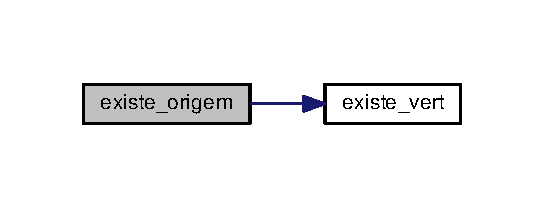
\includegraphics[width=261pt]{grafo__priv_8h_aa7c7803e91592a28e4c0a85112b53fb8_cgraph}
\end{center}
\end{figure}




Este é o diagrama das funções que utilizam esta função\+:
\nopagebreak
\begin{figure}[H]
\begin{center}
\leavevmode
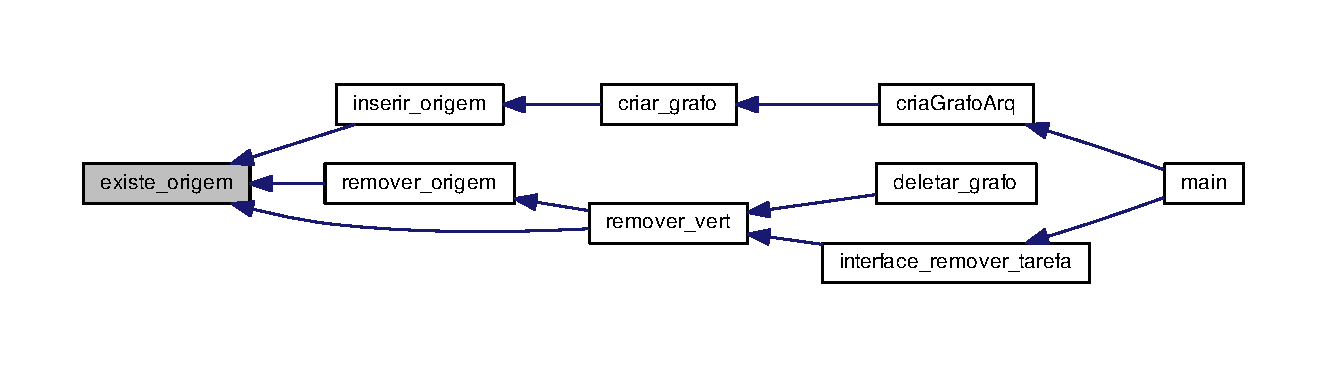
\includegraphics[width=350pt]{grafo__priv_8h_aa7c7803e91592a28e4c0a85112b53fb8_icgraph}
\end{center}
\end{figure}


\hypertarget{grafo__priv_8h_adc1a8c08d13a78eda202bc49275712f5}{}\index{grafo\+\_\+priv.\+h@{grafo\+\_\+priv.\+h}!inserir\+\_\+origem@{inserir\+\_\+origem}}
\index{inserir\+\_\+origem@{inserir\+\_\+origem}!grafo\+\_\+priv.\+h@{grafo\+\_\+priv.\+h}}
\subsubsection[{inserir\+\_\+origem(grafo\+\_\+priv\+\_\+t $\ast$meu\+\_\+grafo, Celula\+\_\+priv\+\_\+t $\ast$celula)}]{\setlength{\rightskip}{0pt plus 5cm}void inserir\+\_\+origem (
\begin{DoxyParamCaption}
\item[{{\bf grafo\+\_\+priv\+\_\+t} $\ast$}]{meu\+\_\+grafo, }
\item[{{\bf Celula\+\_\+priv\+\_\+t} $\ast$}]{celula}
\end{DoxyParamCaption}
)}\label{grafo__priv_8h_adc1a8c08d13a78eda202bc49275712f5}


Definição na linha 184 do arquivo grafo.\+cpp.



Referências achar\+\_\+id(), lista\+\_\+origem\+::destino, existe\+\_\+origem(), existe\+\_\+vert(), F\+A\+L\+S\+E\+\_\+\+T, lista\+\_\+vert\+::id, Celula\+\_\+priv\+::id\+\_\+externo, lista\+\_\+vert\+::next, lista\+\_\+origem\+::next, Celula\+\_\+priv\+::nome, grafo\+\_\+priv\+::origem, T\+R\+U\+E\+\_\+\+T e grafo\+\_\+priv\+::vert.



Referenciado por criar\+\_\+grafo().



Este é o diagrama das funções utilizadas por esta função\+:
\nopagebreak
\begin{figure}[H]
\begin{center}
\leavevmode
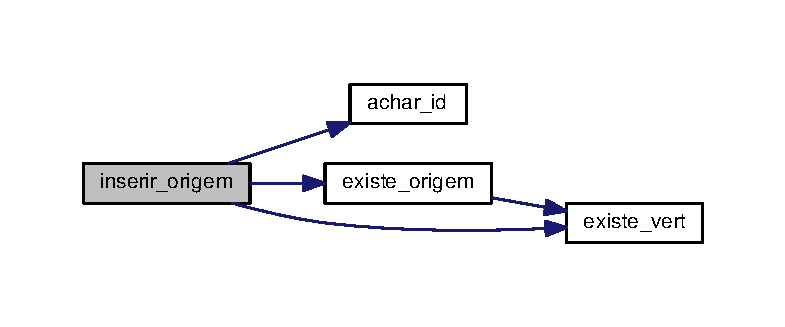
\includegraphics[width=350pt]{grafo__priv_8h_adc1a8c08d13a78eda202bc49275712f5_cgraph}
\end{center}
\end{figure}




Este é o diagrama das funções que utilizam esta função\+:
\nopagebreak
\begin{figure}[H]
\begin{center}
\leavevmode
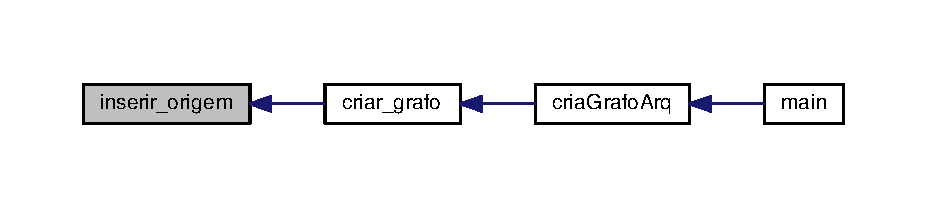
\includegraphics[width=335pt]{grafo__priv_8h_adc1a8c08d13a78eda202bc49275712f5_icgraph}
\end{center}
\end{figure}


\hypertarget{grafo__priv_8h_a2f6600bf1f6ecc3c960e244f3e7b5c8f}{}\index{grafo\+\_\+priv.\+h@{grafo\+\_\+priv.\+h}!remover\+\_\+origem@{remover\+\_\+origem}}
\index{remover\+\_\+origem@{remover\+\_\+origem}!grafo\+\_\+priv.\+h@{grafo\+\_\+priv.\+h}}
\subsubsection[{remover\+\_\+origem(grafo\+\_\+priv\+\_\+t $\ast$meu\+\_\+grafo, int id\+\_\+externo)}]{\setlength{\rightskip}{0pt plus 5cm}void remover\+\_\+origem (
\begin{DoxyParamCaption}
\item[{{\bf grafo\+\_\+priv\+\_\+t} $\ast$}]{meu\+\_\+grafo, }
\item[{int}]{id\+\_\+externo}
\end{DoxyParamCaption}
)}\label{grafo__priv_8h_a2f6600bf1f6ecc3c960e244f3e7b5c8f}


Definição na linha 395 do arquivo grafo.\+cpp.



Referências achar\+\_\+id(), lista\+\_\+origem\+::destino, existe\+\_\+origem(), existe\+\_\+vert(), lista\+\_\+vert\+::id, lista\+\_\+origem\+::next, grafo\+\_\+priv\+::origem e T\+R\+U\+E\+\_\+\+T.



Referenciado por remover\+\_\+vert().



Este é o diagrama das funções utilizadas por esta função\+:
\nopagebreak
\begin{figure}[H]
\begin{center}
\leavevmode
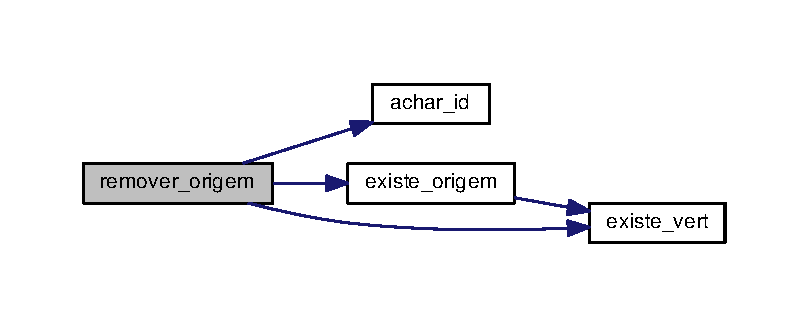
\includegraphics[width=350pt]{grafo__priv_8h_a2f6600bf1f6ecc3c960e244f3e7b5c8f_cgraph}
\end{center}
\end{figure}




Este é o diagrama das funções que utilizam esta função\+:
\nopagebreak
\begin{figure}[H]
\begin{center}
\leavevmode
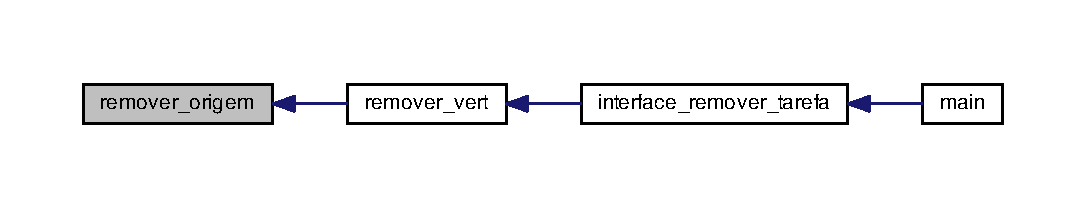
\includegraphics[width=350pt]{grafo__priv_8h_a2f6600bf1f6ecc3c960e244f3e7b5c8f_icgraph}
\end{center}
\end{figure}



\hypertarget{grafo_8cpp}{}\section{Referência do Arquivo grafo.\+cpp}
\label{grafo_8cpp}\index{grafo.\+cpp@{grafo.\+cpp}}
{\ttfamily \#include $<$stdio.\+h$>$}\\*
{\ttfamily \#include $<$stdlib.\+h$>$}\\*
{\ttfamily \#include $<$string.\+h$>$}\\*
{\ttfamily \#include \char`\"{}grafo\+\_\+priv.\+h\char`\"{}}\\*
{\ttfamily \#include \char`\"{}grafo.\+h\char`\"{}}\\*
{\ttfamily \#include $<$algorithm$>$}\\*
{\ttfamily \#include $<$curses.\+h$>$}\\*
Gráfico de dependência de inclusões para grafo.\+cpp\+:\nopagebreak
\begin{figure}[H]
\begin{center}
\leavevmode
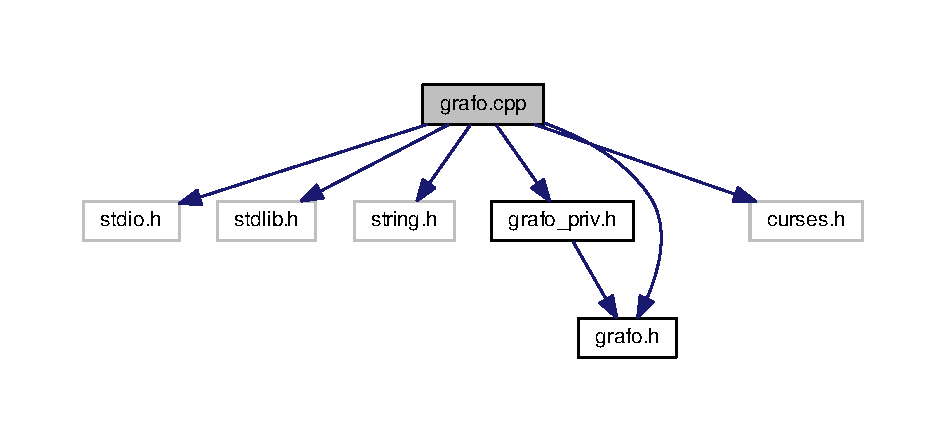
\includegraphics[width=350pt]{grafo_8cpp__incl}
\end{center}
\end{figure}
\subsection*{Definições e Macros}
\begin{DoxyCompactItemize}
\item 
\#define \hyperlink{grafo_8cpp_ad72dbcf6d0153db1b8d8a58001feed83}{D\+E\+B\+U\+G}
\end{DoxyCompactItemize}
\subsection*{Funções}
\begin{DoxyCompactItemize}
\item 
\hyperlink{grafo_8h_a282167c584dceb79dde5c159a85b685b}{grafo\+\_\+priv\+\_\+t} $\ast$ \hyperlink{grafo_8cpp_a3e61bf2ada0f9af7e2e9883241496606}{criar\+\_\+grafo} (void)
\begin{DoxyCompactList}\small\item\em Cria grafo. \end{DoxyCompactList}\item 
\hyperlink{grafo_8h_a282167c584dceb79dde5c159a85b685b}{grafo\+\_\+priv\+\_\+t} $\ast$ \hyperlink{grafo_8cpp_af4f0fbcdd746c0f494e9601a83ddc9fe}{deletar\+\_\+grafo} (\hyperlink{grafo_8h_a282167c584dceb79dde5c159a85b685b}{grafo\+\_\+priv\+\_\+t} $\ast$meu\+\_\+grafo)
\begin{DoxyCompactList}\small\item\em Deleta grafo. \end{DoxyCompactList}\item 
\hyperlink{grafo_8h_a64f906a639abdfda7fffa9ace7e4c286}{resposta} \hyperlink{grafo_8cpp_ac70f5a4fd6ff7c6913f0ce99de099263}{existe\+\_\+vert} (const \hyperlink{grafo_8h_a282167c584dceb79dde5c159a85b685b}{grafo\+\_\+priv\+\_\+t} $\ast$meu\+\_\+grafo, int id\+\_\+externo)
\item 
\hyperlink{grafo_8h_a64f906a639abdfda7fffa9ace7e4c286}{resposta} \hyperlink{grafo_8cpp_aa7c7803e91592a28e4c0a85112b53fb8}{existe\+\_\+origem} (const \hyperlink{grafo_8h_a282167c584dceb79dde5c159a85b685b}{grafo\+\_\+priv\+\_\+t} $\ast$meu\+\_\+grafo, int id\+\_\+externo)
\item 
\hyperlink{grafo_8h_a64f906a639abdfda7fffa9ace7e4c286}{resposta} \hyperlink{grafo_8cpp_a56edc294bdf9e834989d9c8d31ed3a64}{existe\+\_\+aresta} (const \hyperlink{grafo_8h_a282167c584dceb79dde5c159a85b685b}{grafo\+\_\+priv\+\_\+t} $\ast$meu\+\_\+grafo, int id\+\_\+externo1, int id\+\_\+externo2)
\item 
int \hyperlink{grafo_8cpp_ac428ee7436d16b5251b093aa79183fda}{achar\+\_\+id} (const \hyperlink{grafo_8h_a282167c584dceb79dde5c159a85b685b}{grafo\+\_\+priv\+\_\+t} $\ast$meu\+\_\+grafo, int id\+\_\+externo)
\item 
\hyperlink{grafo_8h_ac2219b5d1f94e440b5895ce440ab23b9}{Celula\+\_\+priv\+\_\+t} $\ast$ \hyperlink{grafo_8cpp_a90390d2135067928e2c69cd964c9bec5}{achar\+\_\+celula} (const \hyperlink{grafo_8h_a282167c584dceb79dde5c159a85b685b}{grafo\+\_\+priv\+\_\+t} $\ast$meu\+\_\+grafo, int id\+\_\+externo)
\item 
void \hyperlink{grafo_8cpp_a659b567cb7e165b526b6fe05a433452e}{inserir\+\_\+vert} (\hyperlink{grafo_8h_a282167c584dceb79dde5c159a85b685b}{grafo\+\_\+priv\+\_\+t} $\ast$meu\+\_\+grafo, \hyperlink{grafo_8h_ac2219b5d1f94e440b5895ce440ab23b9}{Celula\+\_\+priv\+\_\+t} $\ast$celula)
\item 
void \hyperlink{grafo_8cpp_adc1a8c08d13a78eda202bc49275712f5}{inserir\+\_\+origem} (\hyperlink{grafo_8h_a282167c584dceb79dde5c159a85b685b}{grafo\+\_\+priv\+\_\+t} $\ast$meu\+\_\+grafo, \hyperlink{grafo_8h_ac2219b5d1f94e440b5895ce440ab23b9}{Celula\+\_\+priv\+\_\+t} $\ast$celula)
\item 
void \hyperlink{grafo_8cpp_a0e69707897c891bf77319d494cae8f26}{inserir\+\_\+aresta} (\hyperlink{grafo_8h_a282167c584dceb79dde5c159a85b685b}{grafo\+\_\+priv\+\_\+t} $\ast$meu\+\_\+grafo, int id\+\_\+externo1, \hyperlink{grafo_8h_ac2219b5d1f94e440b5895ce440ab23b9}{Celula\+\_\+priv\+\_\+t} $\ast$celula2, int peso)
\item 
void \hyperlink{grafo_8cpp_a2812c8a1cbeaab16d0aaa6da10ec4372}{remover\+\_\+vert} (\hyperlink{grafo_8h_a282167c584dceb79dde5c159a85b685b}{grafo\+\_\+priv\+\_\+t} $\ast$meu\+\_\+grafo, int id\+\_\+externo)
\item 
void \hyperlink{grafo_8cpp_a2f6600bf1f6ecc3c960e244f3e7b5c8f}{remover\+\_\+origem} (\hyperlink{grafo_8h_a282167c584dceb79dde5c159a85b685b}{grafo\+\_\+priv\+\_\+t} $\ast$meu\+\_\+grafo, int id\+\_\+externo)
\item 
void \hyperlink{grafo_8cpp_ac16199e4256247b546b67d6d881be137}{remover\+\_\+aresta} (\hyperlink{grafo_8h_a282167c584dceb79dde5c159a85b685b}{grafo\+\_\+priv\+\_\+t} $\ast$meu\+\_\+grafo, int id\+\_\+externo1, int id\+\_\+externo2)
\item 
int \hyperlink{grafo_8cpp_a5bedfb800e326da354b0403421e0d1ef}{maior\+\_\+id} (const \hyperlink{grafo_8h_a282167c584dceb79dde5c159a85b685b}{grafo\+\_\+priv\+\_\+t} $\ast$meu\+\_\+grafo)
\item 
int \hyperlink{grafo_8cpp_a31c64875fe3134ba04439feb7d119cf3}{num\+\_\+vert} (const \hyperlink{grafo_8h_a282167c584dceb79dde5c159a85b685b}{grafo\+\_\+priv\+\_\+t} $\ast$meu\+\_\+grafo)
\item 
int \hyperlink{grafo_8cpp_ac94be03e94792b9b868abb38c7e17e36}{num\+\_\+arestas} (const \hyperlink{grafo_8h_a282167c584dceb79dde5c159a85b685b}{grafo\+\_\+priv\+\_\+t} $\ast$meu\+\_\+grafo)
\item 
int \hyperlink{grafo_8cpp_ad507a38f9feef6cad69436ec774b535f}{menor\+\_\+caminho} (const \hyperlink{grafo_8h_a282167c584dceb79dde5c159a85b685b}{grafo\+\_\+priv\+\_\+t} $\ast$meu\+\_\+grafo, int $\ast$$\ast$dist)
\item 
int \hyperlink{grafo_8cpp_a8081c2a1fc44913609de1a49fb491c3b}{dfs} (const \hyperlink{grafo_8h_a282167c584dceb79dde5c159a85b685b}{grafo\+\_\+priv\+\_\+t} $\ast$meu\+\_\+grafo, \hyperlink{grafo__priv_8h_aecb68281fecb412bf6427dd6a07d5077}{lista\+\_\+vert\+\_\+t} $\ast$atual, int $\ast$marc)
\item 
\hyperlink{grafo_8h_a64f906a639abdfda7fffa9ace7e4c286}{resposta} \hyperlink{grafo_8cpp_a46f8363c4da6edf056e5fffba46e1bc7}{eh\+\_\+conexo} (const \hyperlink{grafo_8h_a282167c584dceb79dde5c159a85b685b}{grafo\+\_\+priv\+\_\+t} $\ast$meu\+\_\+grafo)
\item 
void \hyperlink{grafo_8cpp_a1dd7cc6696ade339827db4d2019239fc}{Imprime\+\_\+\+Tarefas} (const \hyperlink{grafo_8h_a282167c584dceb79dde5c159a85b685b}{grafo\+\_\+priv\+\_\+t} $\ast$meu\+\_\+grafo, int linha, int coluna)
\item 
void \hyperlink{grafo_8cpp_aadbd57b376954aeeb119120d5a4a196f}{Grava\+\_\+\+Arq} (\hyperlink{grafo_8h_a282167c584dceb79dde5c159a85b685b}{grafo\+\_\+priv\+\_\+t} $\ast$meu\+\_\+grafo, char $\ast$Nome\+Arq)
\item 
void \hyperlink{grafo_8cpp_a79154a07716d283ad68106cf54beaf07}{editar\+\_\+celula} (\hyperlink{grafo_8h_a282167c584dceb79dde5c159a85b685b}{grafo\+\_\+priv\+\_\+t} $\ast$meu\+\_\+grafo, int I\+D)
\item 
int \hyperlink{grafo_8cpp_a14183876086781302e2d81ab2457dc4e}{tempo\+\_\+minimo} (const \hyperlink{grafo_8h_a282167c584dceb79dde5c159a85b685b}{grafo\+\_\+priv\+\_\+t} $\ast$meu\+\_\+grafo, int id\+\_\+fim)
\item 
void \hyperlink{grafo_8cpp_acb5b55f7d1508a1b35b76e43bc817623}{ja\+\_\+feito} (const \hyperlink{grafo_8h_a282167c584dceb79dde5c159a85b685b}{grafo\+\_\+priv\+\_\+t} $\ast$meu\+\_\+grafo, int d)
\item 
\hyperlink{grafo_8h_a282167c584dceb79dde5c159a85b685b}{grafo\+\_\+priv\+\_\+t} $\ast$ \hyperlink{grafo_8cpp_a1bb7038cecd5aa54025b6c5931bc0205}{cria\+Grafo\+Arq} (char $\ast$nome\+Arq)
\end{DoxyCompactItemize}


\subsection{Definições e macros}
\hypertarget{grafo_8cpp_ad72dbcf6d0153db1b8d8a58001feed83}{}\index{grafo.\+cpp@{grafo.\+cpp}!D\+E\+B\+U\+G@{D\+E\+B\+U\+G}}
\index{D\+E\+B\+U\+G@{D\+E\+B\+U\+G}!grafo.\+cpp@{grafo.\+cpp}}
\subsubsection[{D\+E\+B\+U\+G}]{\setlength{\rightskip}{0pt plus 5cm}\#define D\+E\+B\+U\+G}\label{grafo_8cpp_ad72dbcf6d0153db1b8d8a58001feed83}


Definição na linha 13 do arquivo grafo.\+cpp.



\subsection{Funções}
\hypertarget{grafo_8cpp_a90390d2135067928e2c69cd964c9bec5}{}\index{grafo.\+cpp@{grafo.\+cpp}!achar\+\_\+celula@{achar\+\_\+celula}}
\index{achar\+\_\+celula@{achar\+\_\+celula}!grafo.\+cpp@{grafo.\+cpp}}
\subsubsection[{achar\+\_\+celula(const grafo\+\_\+priv\+\_\+t $\ast$meu\+\_\+grafo, int id\+\_\+externo)}]{\setlength{\rightskip}{0pt plus 5cm}{\bf Celula\+\_\+priv\+\_\+t}$\ast$ achar\+\_\+celula (
\begin{DoxyParamCaption}
\item[{const {\bf grafo\+\_\+priv\+\_\+t} $\ast$}]{meu\+\_\+grafo, }
\item[{int}]{id\+\_\+externo}
\end{DoxyParamCaption}
)}\label{grafo_8cpp_a90390d2135067928e2c69cd964c9bec5}


Definição na linha 99 do arquivo grafo.\+cpp.



Referências lista\+\_\+vert\+\_\+codigo\+::dado, Celula\+\_\+priv\+::id\+\_\+externo, lista\+\_\+vert\+\_\+codigo\+::next e grafo\+\_\+priv\+::tabela.



Referenciado por editar\+\_\+celula(), interface\+\_\+vizualizar\+\_\+determinada\+\_\+tarefa() e menor\+\_\+caminho().



Este é o diagrama das funções que utilizam esta função\+:\nopagebreak
\begin{figure}[H]
\begin{center}
\leavevmode
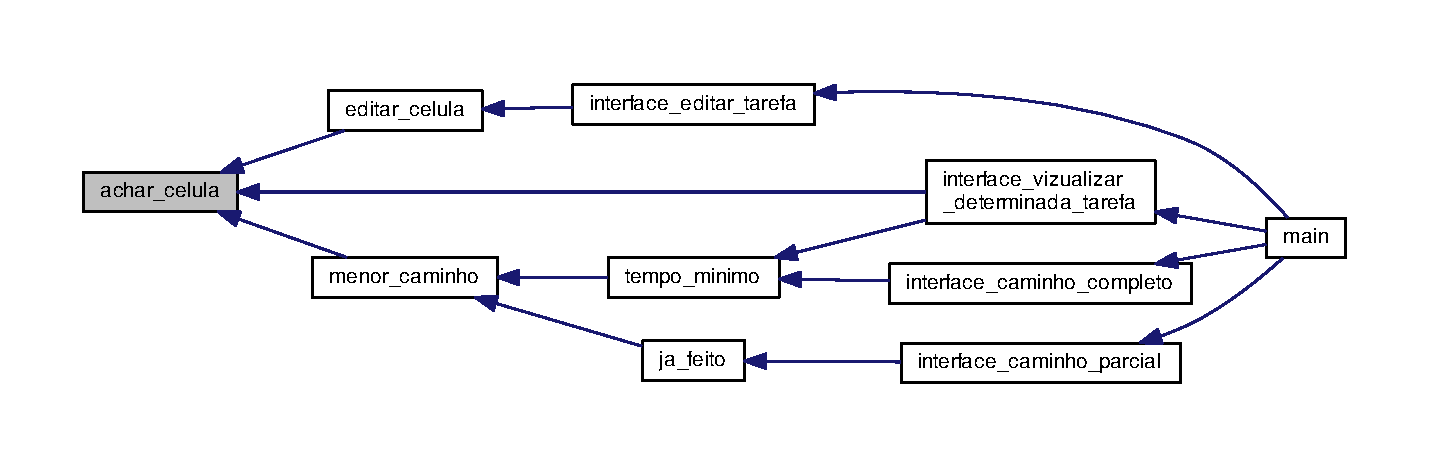
\includegraphics[width=350pt]{grafo_8cpp_a90390d2135067928e2c69cd964c9bec5_icgraph}
\end{center}
\end{figure}


\hypertarget{grafo_8cpp_ac428ee7436d16b5251b093aa79183fda}{}\index{grafo.\+cpp@{grafo.\+cpp}!achar\+\_\+id@{achar\+\_\+id}}
\index{achar\+\_\+id@{achar\+\_\+id}!grafo.\+cpp@{grafo.\+cpp}}
\subsubsection[{achar\+\_\+id(const grafo\+\_\+priv\+\_\+t $\ast$meu\+\_\+grafo, int id\+\_\+externo)}]{\setlength{\rightskip}{0pt plus 5cm}int achar\+\_\+id (
\begin{DoxyParamCaption}
\item[{const {\bf grafo\+\_\+priv\+\_\+t} $\ast$}]{meu\+\_\+grafo, }
\item[{int}]{id\+\_\+externo}
\end{DoxyParamCaption}
)}\label{grafo_8cpp_ac428ee7436d16b5251b093aa79183fda}


Definição na linha 89 do arquivo grafo.\+cpp.



Referências lista\+\_\+vert\+\_\+codigo\+::dado, lista\+\_\+vert\+\_\+codigo\+::id, Celula\+\_\+priv\+::id\+\_\+externo, lista\+\_\+vert\+\_\+codigo\+::next e grafo\+\_\+priv\+::tabela.



Referenciado por inserir\+\_\+aresta(), inserir\+\_\+origem(), menor\+\_\+caminho(), remover\+\_\+aresta(), remover\+\_\+origem() e remover\+\_\+vert().



Este é o diagrama das funções que utilizam esta função\+:
\nopagebreak
\begin{figure}[H]
\begin{center}
\leavevmode
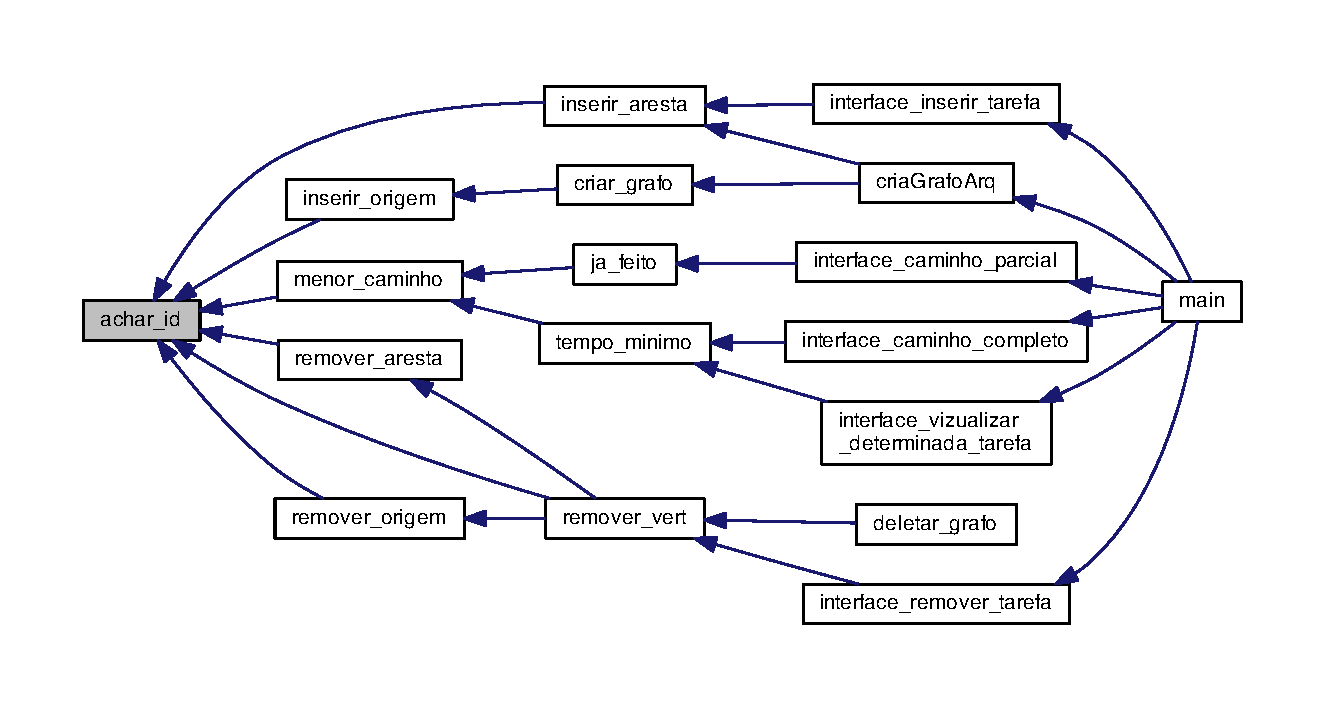
\includegraphics[width=350pt]{grafo_8cpp_ac428ee7436d16b5251b093aa79183fda_icgraph}
\end{center}
\end{figure}


\hypertarget{grafo_8cpp_a1bb7038cecd5aa54025b6c5931bc0205}{}\index{grafo.\+cpp@{grafo.\+cpp}!cria\+Grafo\+Arq@{cria\+Grafo\+Arq}}
\index{cria\+Grafo\+Arq@{cria\+Grafo\+Arq}!grafo.\+cpp@{grafo.\+cpp}}
\subsubsection[{cria\+Grafo\+Arq(char $\ast$nome\+Arq)}]{\setlength{\rightskip}{0pt plus 5cm}{\bf grafo\+\_\+priv\+\_\+t}$\ast$ cria\+Grafo\+Arq (
\begin{DoxyParamCaption}
\item[{char $\ast$}]{nome\+Arq}
\end{DoxyParamCaption}
)}\label{grafo_8cpp_a1bb7038cecd5aa54025b6c5931bc0205}


Definição na linha 732 do arquivo grafo.\+cpp.



Referências criar\+\_\+grafo(), Celula\+\_\+priv\+::duracao, Celula\+\_\+priv\+::executada, Celula\+\_\+priv\+::id\+\_\+externo, Celula\+\_\+priv\+::ini\+\_\+min, inserir\+\_\+aresta(), inserir\+\_\+vert(), Celula\+\_\+priv\+::nome, Celula\+\_\+priv\+::pre\+\_\+req e Celula\+\_\+priv\+::reqs.



Referenciado por main().



Este é o diagrama das funções utilizadas por esta função\+:
\nopagebreak
\begin{figure}[H]
\begin{center}
\leavevmode
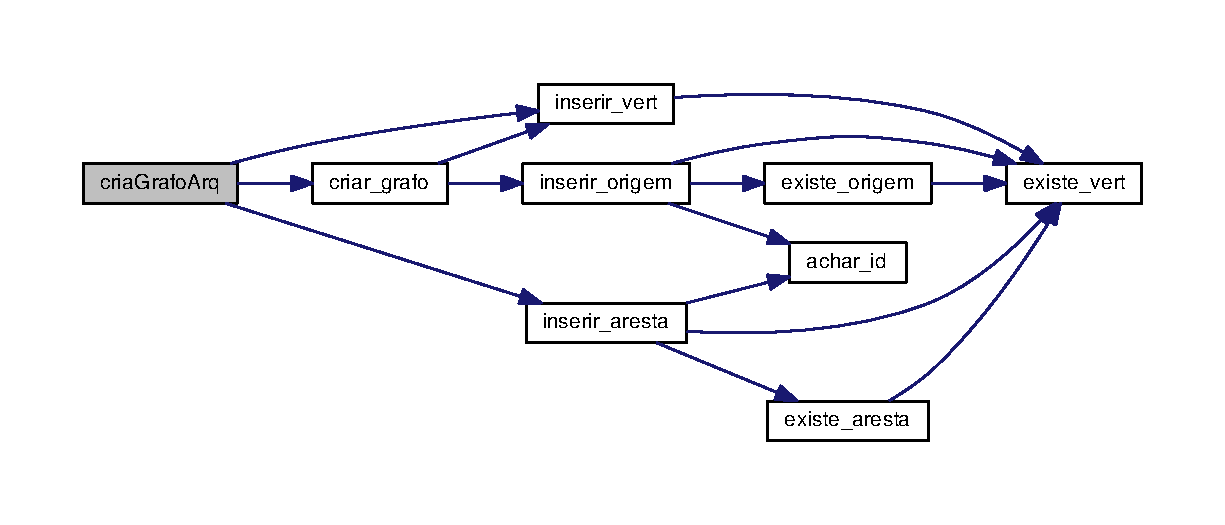
\includegraphics[width=350pt]{grafo_8cpp_a1bb7038cecd5aa54025b6c5931bc0205_cgraph}
\end{center}
\end{figure}




Este é o diagrama das funções que utilizam esta função\+:
\nopagebreak
\begin{figure}[H]
\begin{center}
\leavevmode
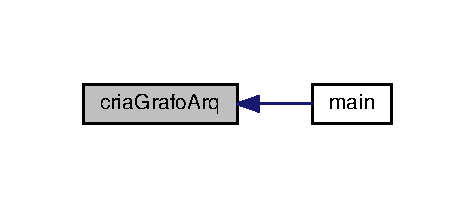
\includegraphics[width=228pt]{grafo_8cpp_a1bb7038cecd5aa54025b6c5931bc0205_icgraph}
\end{center}
\end{figure}


\hypertarget{grafo_8cpp_a3e61bf2ada0f9af7e2e9883241496606}{}\index{grafo.\+cpp@{grafo.\+cpp}!criar\+\_\+grafo@{criar\+\_\+grafo}}
\index{criar\+\_\+grafo@{criar\+\_\+grafo}!grafo.\+cpp@{grafo.\+cpp}}
\subsubsection[{criar\+\_\+grafo(void)}]{\setlength{\rightskip}{0pt plus 5cm}{\bf grafo\+\_\+priv\+\_\+t}$\ast$ criar\+\_\+grafo (
\begin{DoxyParamCaption}
\item[{void}]{}
\end{DoxyParamCaption}
)}\label{grafo_8cpp_a3e61bf2ada0f9af7e2e9883241496606}


Cria grafo. 

\hypertarget{grafo_8cpp_desc}{}\subsection{Descrição}\label{grafo_8cpp_desc}
Aloca a memória necessária e inicializa um grafo \hypertarget{grafo_8cpp_para}{}\subsection{Parâmetros}\label{grafo_8cpp_para}
Não ha parâmetros, a alocação e inicializam não dependem de nenhum parâmetro do usuário

\begin{DoxyReturn}{Retorna}
Se retorna um ponteiro para a grafo criado
\end{DoxyReturn}
\hypertarget{grafo_8cpp_assert}{}\subsection{Assertiva de saída}\label{grafo_8cpp_assert}
O grafo gerado é consistente e não possui nenhum vértice, origem ou aresta. 

Definição na linha 15 do arquivo grafo.\+cpp.



Referências Celula\+\_\+priv\+::executada, Celula\+\_\+priv\+::id\+\_\+externo, Celula\+\_\+priv\+::ini\+\_\+min, inserir\+\_\+origem(), inserir\+\_\+vert(), Celula\+\_\+priv\+::nome, grafo\+\_\+priv\+::origem, Celula\+\_\+priv\+::pre\+\_\+req, grafo\+\_\+priv\+::tabela e grafo\+\_\+priv\+::vert.



Referenciado por cria\+Grafo\+Arq().



Este é o diagrama das funções utilizadas por esta função\+:\nopagebreak
\begin{figure}[H]
\begin{center}
\leavevmode
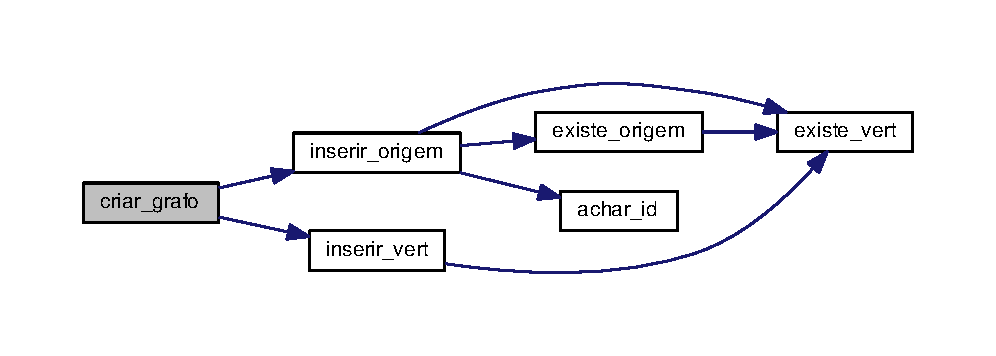
\includegraphics[width=350pt]{grafo_8cpp_a3e61bf2ada0f9af7e2e9883241496606_cgraph}
\end{center}
\end{figure}




Este é o diagrama das funções que utilizam esta função\+:
\nopagebreak
\begin{figure}[H]
\begin{center}
\leavevmode
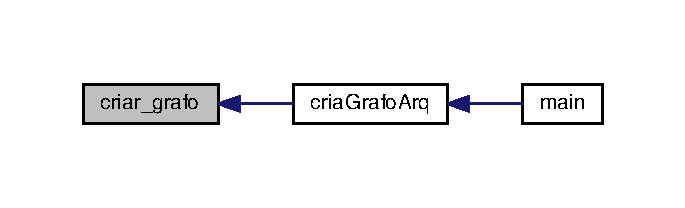
\includegraphics[width=329pt]{grafo_8cpp_a3e61bf2ada0f9af7e2e9883241496606_icgraph}
\end{center}
\end{figure}


\hypertarget{grafo_8cpp_af4f0fbcdd746c0f494e9601a83ddc9fe}{}\index{grafo.\+cpp@{grafo.\+cpp}!deletar\+\_\+grafo@{deletar\+\_\+grafo}}
\index{deletar\+\_\+grafo@{deletar\+\_\+grafo}!grafo.\+cpp@{grafo.\+cpp}}
\subsubsection[{deletar\+\_\+grafo(grafo\+\_\+priv\+\_\+t $\ast$meu\+\_\+grafo)}]{\setlength{\rightskip}{0pt plus 5cm}{\bf grafo\+\_\+priv\+\_\+t}$\ast$ deletar\+\_\+grafo (
\begin{DoxyParamCaption}
\item[{{\bf grafo\+\_\+priv\+\_\+t} $\ast$}]{meu\+\_\+grafo}
\end{DoxyParamCaption}
)}\label{grafo_8cpp_af4f0fbcdd746c0f494e9601a83ddc9fe}


Deleta grafo. 

\hypertarget{grafo_8cpp_desc}{}\subsection{Descrição}\label{grafo_8cpp_desc}
Desaloca toda a memória utilizada pelo grafo


\begin{DoxyParams}{Parâmetros}
{\em meu\+\_\+grafo} & -\/ Deve ser passado um ponteiro para um grafo inicializado\\
\hline
\end{DoxyParams}
\begin{DoxyReturn}{Retorna}
Retorna um ponteiro para o grafo, que será N\+U\+L\+L. O valor de retorno é muito importante, uma vez que se ele não for utilizado o grafo do usuário apontará para um endereço não alocado e qualquer tentativa de utilizá-\/lo poderá gerar erros no sistema. Caso o grafo passado não tenha sido inicializado, o programa poderá parar a execução
\end{DoxyReturn}
\hypertarget{grafo_8cpp_assert}{}\subsection{Assertiva de saída}\label{grafo_8cpp_assert}
O grafo já deve ter sido inicializado por \hyperlink{grafo_8h_a3e61bf2ada0f9af7e2e9883241496606}{criar\+\_\+grafo()} Assertiva de saída Se retornará um ponteiro para o mesmo grafo passado, após a deleção que será N\+U\+L\+L. 

Definição na linha 35 do arquivo grafo.\+cpp.



Referências grafo\+\_\+priv\+::tabela.

\hypertarget{grafo_8cpp_a8081c2a1fc44913609de1a49fb491c3b}{}\index{grafo.\+cpp@{grafo.\+cpp}!dfs@{dfs}}
\index{dfs@{dfs}!grafo.\+cpp@{grafo.\+cpp}}
\subsubsection[{dfs(const grafo\+\_\+priv\+\_\+t $\ast$meu\+\_\+grafo, lista\+\_\+vert\+\_\+t $\ast$atual, int $\ast$marc)}]{\setlength{\rightskip}{0pt plus 5cm}int dfs (
\begin{DoxyParamCaption}
\item[{const {\bf grafo\+\_\+priv\+\_\+t} $\ast$}]{meu\+\_\+grafo, }
\item[{{\bf lista\+\_\+vert\+\_\+t} $\ast$}]{atual, }
\item[{int $\ast$}]{marc}
\end{DoxyParamCaption}
)}\label{grafo_8cpp_a8081c2a1fc44913609de1a49fb491c3b}


Definição na linha 544 do arquivo grafo.\+cpp.



Referências lista\+\_\+aresta\+::destino, lista\+\_\+vert\+::id, lista\+\_\+aresta\+::next e lista\+\_\+vert\+::sucessores.



Referenciado por eh\+\_\+conexo().



Este é o diagrama das funções que utilizam esta função\+:\nopagebreak
\begin{figure}[H]
\begin{center}
\leavevmode
\includegraphics[width=213pt]{grafo_8cpp_a8081c2a1fc44913609de1a49fb491c3b_icgraph}
\end{center}
\end{figure}


\hypertarget{grafo_8cpp_a79154a07716d283ad68106cf54beaf07}{}\index{grafo.\+cpp@{grafo.\+cpp}!editar\+\_\+celula@{editar\+\_\+celula}}
\index{editar\+\_\+celula@{editar\+\_\+celula}!grafo.\+cpp@{grafo.\+cpp}}
\subsubsection[{editar\+\_\+celula(grafo\+\_\+priv\+\_\+t $\ast$meu\+\_\+grafo, int I\+D)}]{\setlength{\rightskip}{0pt plus 5cm}void editar\+\_\+celula (
\begin{DoxyParamCaption}
\item[{{\bf grafo\+\_\+priv\+\_\+t} $\ast$}]{meu\+\_\+grafo, }
\item[{int}]{I\+D}
\end{DoxyParamCaption}
)}\label{grafo_8cpp_a79154a07716d283ad68106cf54beaf07}


Definição na linha 641 do arquivo grafo.\+cpp.



Referências achar\+\_\+celula(), Celula\+\_\+priv\+::duracao, Celula\+\_\+priv\+::executada, Celula\+\_\+priv\+::id\+\_\+externo, Celula\+\_\+priv\+::ini\+\_\+min, Celula\+\_\+priv\+::nome, Celula\+\_\+priv\+::pre\+\_\+req e Celula\+\_\+priv\+::reqs.



Referenciado por interface\+\_\+editar\+\_\+tarefa().



Este é o diagrama das funções utilizadas por esta função\+:\nopagebreak
\begin{figure}[H]
\begin{center}
\leavevmode
\includegraphics[width=264pt]{grafo_8cpp_a79154a07716d283ad68106cf54beaf07_cgraph}
\end{center}
\end{figure}




Este é o diagrama das funções que utilizam esta função\+:\nopagebreak
\begin{figure}[H]
\begin{center}
\leavevmode
\includegraphics[width=350pt]{grafo_8cpp_a79154a07716d283ad68106cf54beaf07_icgraph}
\end{center}
\end{figure}


\hypertarget{grafo_8cpp_a46f8363c4da6edf056e5fffba46e1bc7}{}\index{grafo.\+cpp@{grafo.\+cpp}!eh\+\_\+conexo@{eh\+\_\+conexo}}
\index{eh\+\_\+conexo@{eh\+\_\+conexo}!grafo.\+cpp@{grafo.\+cpp}}
\subsubsection[{eh\+\_\+conexo(const grafo\+\_\+priv\+\_\+t $\ast$meu\+\_\+grafo)}]{\setlength{\rightskip}{0pt plus 5cm}{\bf resposta} eh\+\_\+conexo (
\begin{DoxyParamCaption}
\item[{const {\bf grafo\+\_\+priv\+\_\+t} $\ast$}]{meu\+\_\+grafo}
\end{DoxyParamCaption}
)}\label{grafo_8cpp_a46f8363c4da6edf056e5fffba46e1bc7}


Definição na linha 560 do arquivo grafo.\+cpp.



Referências lista\+\_\+origem\+::destino, dfs(), F\+A\+L\+S\+E\+\_\+\+T, lista\+\_\+vert\+::id, maior\+\_\+id(), lista\+\_\+origem\+::next, num\+\_\+vert(), grafo\+\_\+priv\+::origem e T\+R\+U\+E\+\_\+\+T.



Este é o diagrama das funções utilizadas por esta função\+:\nopagebreak
\begin{figure}[H]
\begin{center}
\leavevmode
\includegraphics[width=240pt]{grafo_8cpp_a46f8363c4da6edf056e5fffba46e1bc7_cgraph}
\end{center}
\end{figure}


\hypertarget{grafo_8cpp_a56edc294bdf9e834989d9c8d31ed3a64}{}\index{grafo.\+cpp@{grafo.\+cpp}!existe\+\_\+aresta@{existe\+\_\+aresta}}
\index{existe\+\_\+aresta@{existe\+\_\+aresta}!grafo.\+cpp@{grafo.\+cpp}}
\subsubsection[{existe\+\_\+aresta(const grafo\+\_\+priv\+\_\+t $\ast$meu\+\_\+grafo, int id\+\_\+externo1, int id\+\_\+externo2)}]{\setlength{\rightskip}{0pt plus 5cm}{\bf resposta} existe\+\_\+aresta (
\begin{DoxyParamCaption}
\item[{const {\bf grafo\+\_\+priv\+\_\+t} $\ast$}]{meu\+\_\+grafo, }
\item[{int}]{id\+\_\+externo1, }
\item[{int}]{id\+\_\+externo2}
\end{DoxyParamCaption}
)}\label{grafo_8cpp_a56edc294bdf9e834989d9c8d31ed3a64}


Definição na linha 69 do arquivo grafo.\+cpp.



Referências lista\+\_\+aresta\+::destino, existe\+\_\+vert(), F\+A\+L\+S\+E\+\_\+\+T, lista\+\_\+vert\+::id\+\_\+externo, lista\+\_\+aresta\+::next, lista\+\_\+vert\+::next, lista\+\_\+vert\+::sucessores, T\+R\+U\+E\+\_\+\+T e grafo\+\_\+priv\+::vert.



Referenciado por inserir\+\_\+aresta() e remover\+\_\+aresta().



Este é o diagrama das funções utilizadas por esta função\+:\nopagebreak
\begin{figure}[H]
\begin{center}
\leavevmode
\includegraphics[width=258pt]{grafo_8cpp_a56edc294bdf9e834989d9c8d31ed3a64_cgraph}
\end{center}
\end{figure}




Este é o diagrama das funções que utilizam esta função\+:
\nopagebreak
\begin{figure}[H]
\begin{center}
\leavevmode
\includegraphics[width=350pt]{grafo_8cpp_a56edc294bdf9e834989d9c8d31ed3a64_icgraph}
\end{center}
\end{figure}


\hypertarget{grafo_8cpp_aa7c7803e91592a28e4c0a85112b53fb8}{}\index{grafo.\+cpp@{grafo.\+cpp}!existe\+\_\+origem@{existe\+\_\+origem}}
\index{existe\+\_\+origem@{existe\+\_\+origem}!grafo.\+cpp@{grafo.\+cpp}}
\subsubsection[{existe\+\_\+origem(const grafo\+\_\+priv\+\_\+t $\ast$meu\+\_\+grafo, int id\+\_\+externo)}]{\setlength{\rightskip}{0pt plus 5cm}{\bf resposta} existe\+\_\+origem (
\begin{DoxyParamCaption}
\item[{const {\bf grafo\+\_\+priv\+\_\+t} $\ast$}]{meu\+\_\+grafo, }
\item[{int}]{id\+\_\+externo}
\end{DoxyParamCaption}
)}\label{grafo_8cpp_aa7c7803e91592a28e4c0a85112b53fb8}


Definição na linha 56 do arquivo grafo.\+cpp.



Referências lista\+\_\+origem\+::destino, existe\+\_\+vert(), F\+A\+L\+S\+E\+\_\+\+T, lista\+\_\+vert\+::id\+\_\+externo, lista\+\_\+origem\+::next, grafo\+\_\+priv\+::origem e T\+R\+U\+E\+\_\+\+T.



Referenciado por inserir\+\_\+origem(), remover\+\_\+origem() e remover\+\_\+vert().



Este é o diagrama das funções utilizadas por esta função\+:\nopagebreak
\begin{figure}[H]
\begin{center}
\leavevmode
\includegraphics[width=261pt]{grafo_8cpp_aa7c7803e91592a28e4c0a85112b53fb8_cgraph}
\end{center}
\end{figure}




Este é o diagrama das funções que utilizam esta função\+:
\nopagebreak
\begin{figure}[H]
\begin{center}
\leavevmode
\includegraphics[width=350pt]{grafo_8cpp_aa7c7803e91592a28e4c0a85112b53fb8_icgraph}
\end{center}
\end{figure}


\hypertarget{grafo_8cpp_ac70f5a4fd6ff7c6913f0ce99de099263}{}\index{grafo.\+cpp@{grafo.\+cpp}!existe\+\_\+vert@{existe\+\_\+vert}}
\index{existe\+\_\+vert@{existe\+\_\+vert}!grafo.\+cpp@{grafo.\+cpp}}
\subsubsection[{existe\+\_\+vert(const grafo\+\_\+priv\+\_\+t $\ast$meu\+\_\+grafo, int id\+\_\+externo)}]{\setlength{\rightskip}{0pt plus 5cm}{\bf resposta} existe\+\_\+vert (
\begin{DoxyParamCaption}
\item[{const {\bf grafo\+\_\+priv\+\_\+t} $\ast$}]{meu\+\_\+grafo, }
\item[{int}]{id\+\_\+externo}
\end{DoxyParamCaption}
)}\label{grafo_8cpp_ac70f5a4fd6ff7c6913f0ce99de099263}


Definição na linha 46 do arquivo grafo.\+cpp.



Referências lista\+\_\+vert\+\_\+codigo\+::dado, F\+A\+L\+S\+E\+\_\+\+T, Celula\+\_\+priv\+::id\+\_\+externo, lista\+\_\+vert\+\_\+codigo\+::next, grafo\+\_\+priv\+::tabela e T\+R\+U\+E\+\_\+\+T.



Referenciado por existe\+\_\+aresta(), existe\+\_\+origem(), inserir\+\_\+aresta(), inserir\+\_\+origem(), inserir\+\_\+vert(), remover\+\_\+aresta(), remover\+\_\+origem() e remover\+\_\+vert().



Este é o diagrama das funções que utilizam esta função\+:
\nopagebreak
\begin{figure}[H]
\begin{center}
\leavevmode
\includegraphics[width=350pt]{grafo_8cpp_ac70f5a4fd6ff7c6913f0ce99de099263_icgraph}
\end{center}
\end{figure}


\hypertarget{grafo_8cpp_aadbd57b376954aeeb119120d5a4a196f}{}\index{grafo.\+cpp@{grafo.\+cpp}!Grava\+\_\+\+Arq@{Grava\+\_\+\+Arq}}
\index{Grava\+\_\+\+Arq@{Grava\+\_\+\+Arq}!grafo.\+cpp@{grafo.\+cpp}}
\subsubsection[{Grava\+\_\+\+Arq(grafo\+\_\+priv\+\_\+t $\ast$meu\+\_\+grafo, char $\ast$\+Nome\+Arq)}]{\setlength{\rightskip}{0pt plus 5cm}void Grava\+\_\+\+Arq (
\begin{DoxyParamCaption}
\item[{{\bf grafo\+\_\+priv\+\_\+t} $\ast$}]{meu\+\_\+grafo, }
\item[{char $\ast$}]{Nome\+Arq}
\end{DoxyParamCaption}
)}\label{grafo_8cpp_aadbd57b376954aeeb119120d5a4a196f}


Definição na linha 615 do arquivo grafo.\+cpp.



Referências lista\+\_\+vert\+\_\+codigo\+::dado, Celula\+\_\+priv\+::duracao, Celula\+\_\+priv\+::executada, Celula\+\_\+priv\+::id\+\_\+externo, Celula\+\_\+priv\+::ini\+\_\+min, lista\+\_\+vert\+\_\+codigo\+::next, Celula\+\_\+priv\+::nome, Celula\+\_\+priv\+::pre\+\_\+req, Celula\+\_\+priv\+::reqs e grafo\+\_\+priv\+::tabela.



Referenciado por main().



Este é o diagrama das funções que utilizam esta função\+:\nopagebreak
\begin{figure}[H]
\begin{center}
\leavevmode
\includegraphics[width=220pt]{grafo_8cpp_aadbd57b376954aeeb119120d5a4a196f_icgraph}
\end{center}
\end{figure}


\hypertarget{grafo_8cpp_a1dd7cc6696ade339827db4d2019239fc}{}\index{grafo.\+cpp@{grafo.\+cpp}!Imprime\+\_\+\+Tarefas@{Imprime\+\_\+\+Tarefas}}
\index{Imprime\+\_\+\+Tarefas@{Imprime\+\_\+\+Tarefas}!grafo.\+cpp@{grafo.\+cpp}}
\subsubsection[{Imprime\+\_\+\+Tarefas(const grafo\+\_\+priv\+\_\+t $\ast$meu\+\_\+grafo, int linha, int coluna)}]{\setlength{\rightskip}{0pt plus 5cm}void Imprime\+\_\+\+Tarefas (
\begin{DoxyParamCaption}
\item[{const {\bf grafo\+\_\+priv\+\_\+t} $\ast$}]{meu\+\_\+grafo, }
\item[{int}]{linha, }
\item[{int}]{coluna}
\end{DoxyParamCaption}
)}\label{grafo_8cpp_a1dd7cc6696ade339827db4d2019239fc}


Definição na linha 595 do arquivo grafo.\+cpp.



Referências lista\+\_\+vert\+\_\+codigo\+::dado, Celula\+\_\+priv\+::duracao, Celula\+\_\+priv\+::executada, Celula\+\_\+priv\+::id\+\_\+externo, Celula\+\_\+priv\+::ini\+\_\+min, lista\+\_\+vert\+\_\+codigo\+::next, Celula\+\_\+priv\+::nome, Celula\+\_\+priv\+::pre\+\_\+req, Celula\+\_\+priv\+::reqs e grafo\+\_\+priv\+::tabela.



Referenciado por interface\+\_\+vizualizar\+\_\+tarefas().



Este é o diagrama das funções que utilizam esta função\+:\nopagebreak
\begin{figure}[H]
\begin{center}
\leavevmode
\includegraphics[width=350pt]{grafo_8cpp_a1dd7cc6696ade339827db4d2019239fc_icgraph}
\end{center}
\end{figure}


\hypertarget{grafo_8cpp_a0e69707897c891bf77319d494cae8f26}{}\index{grafo.\+cpp@{grafo.\+cpp}!inserir\+\_\+aresta@{inserir\+\_\+aresta}}
\index{inserir\+\_\+aresta@{inserir\+\_\+aresta}!grafo.\+cpp@{grafo.\+cpp}}
\subsubsection[{inserir\+\_\+aresta(grafo\+\_\+priv\+\_\+t $\ast$meu\+\_\+grafo, int id\+\_\+externo1, Celula\+\_\+priv\+\_\+t $\ast$celula2, int peso)}]{\setlength{\rightskip}{0pt plus 5cm}void inserir\+\_\+aresta (
\begin{DoxyParamCaption}
\item[{{\bf grafo\+\_\+priv\+\_\+t} $\ast$}]{meu\+\_\+grafo, }
\item[{int}]{id\+\_\+externo1, }
\item[{{\bf Celula\+\_\+priv\+\_\+t} $\ast$}]{celula2, }
\item[{int}]{peso}
\end{DoxyParamCaption}
)}\label{grafo_8cpp_a0e69707897c891bf77319d494cae8f26}


Definição na linha 232 do arquivo grafo.\+cpp.



Referências achar\+\_\+id(), lista\+\_\+aresta\+::destino, existe\+\_\+aresta(), existe\+\_\+vert(), F\+A\+L\+S\+E\+\_\+\+T, Celula\+\_\+priv\+::id\+\_\+externo, lista\+\_\+aresta\+::next, lista\+\_\+vert\+::next, Celula\+\_\+priv\+::nome, lista\+\_\+aresta\+::peso, lista\+\_\+vert\+::sucessores, T\+R\+U\+E\+\_\+\+T e grafo\+\_\+priv\+::vert.



Referenciado por cria\+Grafo\+Arq() e interface\+\_\+inserir\+\_\+tarefa().



Este é o diagrama das funções utilizadas por esta função\+:\nopagebreak
\begin{figure}[H]
\begin{center}
\leavevmode
\includegraphics[width=350pt]{grafo_8cpp_a0e69707897c891bf77319d494cae8f26_cgraph}
\end{center}
\end{figure}




Este é o diagrama das funções que utilizam esta função\+:
\nopagebreak
\begin{figure}[H]
\begin{center}
\leavevmode
\includegraphics[width=350pt]{grafo_8cpp_a0e69707897c891bf77319d494cae8f26_icgraph}
\end{center}
\end{figure}


\hypertarget{grafo_8cpp_adc1a8c08d13a78eda202bc49275712f5}{}\index{grafo.\+cpp@{grafo.\+cpp}!inserir\+\_\+origem@{inserir\+\_\+origem}}
\index{inserir\+\_\+origem@{inserir\+\_\+origem}!grafo.\+cpp@{grafo.\+cpp}}
\subsubsection[{inserir\+\_\+origem(grafo\+\_\+priv\+\_\+t $\ast$meu\+\_\+grafo, Celula\+\_\+priv\+\_\+t $\ast$celula)}]{\setlength{\rightskip}{0pt plus 5cm}void inserir\+\_\+origem (
\begin{DoxyParamCaption}
\item[{{\bf grafo\+\_\+priv\+\_\+t} $\ast$}]{meu\+\_\+grafo, }
\item[{{\bf Celula\+\_\+priv\+\_\+t} $\ast$}]{celula}
\end{DoxyParamCaption}
)}\label{grafo_8cpp_adc1a8c08d13a78eda202bc49275712f5}


Definição na linha 184 do arquivo grafo.\+cpp.



Referências achar\+\_\+id(), lista\+\_\+origem\+::destino, existe\+\_\+origem(), existe\+\_\+vert(), F\+A\+L\+S\+E\+\_\+\+T, lista\+\_\+vert\+::id, Celula\+\_\+priv\+::id\+\_\+externo, lista\+\_\+vert\+::next, lista\+\_\+origem\+::next, Celula\+\_\+priv\+::nome, grafo\+\_\+priv\+::origem, T\+R\+U\+E\+\_\+\+T e grafo\+\_\+priv\+::vert.



Referenciado por criar\+\_\+grafo().



Este é o diagrama das funções utilizadas por esta função\+:\nopagebreak
\begin{figure}[H]
\begin{center}
\leavevmode
\includegraphics[width=350pt]{grafo_8cpp_adc1a8c08d13a78eda202bc49275712f5_cgraph}
\end{center}
\end{figure}




Este é o diagrama das funções que utilizam esta função\+:
\nopagebreak
\begin{figure}[H]
\begin{center}
\leavevmode
\includegraphics[width=350pt]{grafo_8cpp_adc1a8c08d13a78eda202bc49275712f5_icgraph}
\end{center}
\end{figure}


\hypertarget{grafo_8cpp_a659b567cb7e165b526b6fe05a433452e}{}\index{grafo.\+cpp@{grafo.\+cpp}!inserir\+\_\+vert@{inserir\+\_\+vert}}
\index{inserir\+\_\+vert@{inserir\+\_\+vert}!grafo.\+cpp@{grafo.\+cpp}}
\subsubsection[{inserir\+\_\+vert(grafo\+\_\+priv\+\_\+t $\ast$meu\+\_\+grafo, Celula\+\_\+priv\+\_\+t $\ast$celula)}]{\setlength{\rightskip}{0pt plus 5cm}void inserir\+\_\+vert (
\begin{DoxyParamCaption}
\item[{{\bf grafo\+\_\+priv\+\_\+t} $\ast$}]{meu\+\_\+grafo, }
\item[{{\bf Celula\+\_\+priv\+\_\+t} $\ast$}]{celula}
\end{DoxyParamCaption}
)}\label{grafo_8cpp_a659b567cb7e165b526b6fe05a433452e}


Definição na linha 110 do arquivo grafo.\+cpp.



Referências lista\+\_\+vert\+::antecessores, existe\+\_\+vert(), F\+A\+L\+S\+E\+\_\+\+T, lista\+\_\+vert\+\_\+codigo\+::id, lista\+\_\+vert\+::id, Celula\+\_\+priv\+::id\+\_\+externo, lista\+\_\+vert\+::id\+\_\+externo, Celula\+\_\+priv\+::ini\+\_\+min, lista\+\_\+vert\+\_\+codigo\+::next, lista\+\_\+vert\+::next, Celula\+\_\+priv\+::nome, Celula\+\_\+priv\+::pre\+\_\+req, lista\+\_\+vert\+::sucessores, grafo\+\_\+priv\+::tabela e grafo\+\_\+priv\+::vert.



Referenciado por cria\+Grafo\+Arq(), criar\+\_\+grafo() e interface\+\_\+inserir\+\_\+tarefa().



Este é o diagrama das funções utilizadas por esta função\+:\nopagebreak
\begin{figure}[H]
\begin{center}
\leavevmode
\includegraphics[width=246pt]{grafo_8cpp_a659b567cb7e165b526b6fe05a433452e_cgraph}
\end{center}
\end{figure}




Este é o diagrama das funções que utilizam esta função\+:
\nopagebreak
\begin{figure}[H]
\begin{center}
\leavevmode
\includegraphics[width=350pt]{grafo_8cpp_a659b567cb7e165b526b6fe05a433452e_icgraph}
\end{center}
\end{figure}


\hypertarget{grafo_8cpp_acb5b55f7d1508a1b35b76e43bc817623}{}\index{grafo.\+cpp@{grafo.\+cpp}!ja\+\_\+feito@{ja\+\_\+feito}}
\index{ja\+\_\+feito@{ja\+\_\+feito}!grafo.\+cpp@{grafo.\+cpp}}
\subsubsection[{ja\+\_\+feito(const grafo\+\_\+priv\+\_\+t $\ast$meu\+\_\+grafo, int d)}]{\setlength{\rightskip}{0pt plus 5cm}void ja\+\_\+feito (
\begin{DoxyParamCaption}
\item[{const {\bf grafo\+\_\+priv\+\_\+t} $\ast$}]{meu\+\_\+grafo, }
\item[{int}]{d}
\end{DoxyParamCaption}
)}\label{grafo_8cpp_acb5b55f7d1508a1b35b76e43bc817623}


Definição na linha 712 do arquivo grafo.\+cpp.



Referências lista\+\_\+vert\+\_\+codigo\+::id, menor\+\_\+caminho(), lista\+\_\+vert\+\_\+codigo\+::next e grafo\+\_\+priv\+::tabela.



Este é o diagrama das funções utilizadas por esta função\+:\nopagebreak
\begin{figure}[H]
\begin{center}
\leavevmode
\includegraphics[width=350pt]{grafo_8cpp_acb5b55f7d1508a1b35b76e43bc817623_cgraph}
\end{center}
\end{figure}


\hypertarget{grafo_8cpp_a5bedfb800e326da354b0403421e0d1ef}{}\index{grafo.\+cpp@{grafo.\+cpp}!maior\+\_\+id@{maior\+\_\+id}}
\index{maior\+\_\+id@{maior\+\_\+id}!grafo.\+cpp@{grafo.\+cpp}}
\subsubsection[{maior\+\_\+id(const grafo\+\_\+priv\+\_\+t $\ast$meu\+\_\+grafo)}]{\setlength{\rightskip}{0pt plus 5cm}int maior\+\_\+id (
\begin{DoxyParamCaption}
\item[{const {\bf grafo\+\_\+priv\+\_\+t} $\ast$}]{meu\+\_\+grafo}
\end{DoxyParamCaption}
)}\label{grafo_8cpp_a5bedfb800e326da354b0403421e0d1ef}


Definição na linha 472 do arquivo grafo.\+cpp.



Referências lista\+\_\+vert\+\_\+codigo\+::id, lista\+\_\+vert\+\_\+codigo\+::next e grafo\+\_\+priv\+::tabela.



Referenciado por eh\+\_\+conexo() e menor\+\_\+caminho().



Este é o diagrama das funções que utilizam esta função\+:\nopagebreak
\begin{figure}[H]
\begin{center}
\leavevmode
\includegraphics[width=350pt]{grafo_8cpp_a5bedfb800e326da354b0403421e0d1ef_icgraph}
\end{center}
\end{figure}


\hypertarget{grafo_8cpp_ad507a38f9feef6cad69436ec774b535f}{}\index{grafo.\+cpp@{grafo.\+cpp}!menor\+\_\+caminho@{menor\+\_\+caminho}}
\index{menor\+\_\+caminho@{menor\+\_\+caminho}!grafo.\+cpp@{grafo.\+cpp}}
\subsubsection[{menor\+\_\+caminho(const grafo\+\_\+priv\+\_\+t $\ast$meu\+\_\+grafo, int $\ast$$\ast$dist)}]{\setlength{\rightskip}{0pt plus 5cm}int menor\+\_\+caminho (
\begin{DoxyParamCaption}
\item[{const {\bf grafo\+\_\+priv\+\_\+t} $\ast$}]{meu\+\_\+grafo, }
\item[{int $\ast$$\ast$}]{dist}
\end{DoxyParamCaption}
)}\label{grafo_8cpp_ad507a38f9feef6cad69436ec774b535f}


Definição na linha 506 do arquivo grafo.\+cpp.



Referências achar\+\_\+celula(), achar\+\_\+id(), lista\+\_\+aresta\+::destino, lista\+\_\+vert\+::id, Celula\+\_\+priv\+::ini\+\_\+min, maior\+\_\+id(), lista\+\_\+aresta\+::next, lista\+\_\+vert\+::next, num\+\_\+vert(), lista\+\_\+aresta\+::peso, lista\+\_\+vert\+::sucessores e grafo\+\_\+priv\+::vert.



Referenciado por ja\+\_\+feito() e tempo\+\_\+minimo().



Este é o diagrama das funções utilizadas por esta função\+:\nopagebreak
\begin{figure}[H]
\begin{center}
\leavevmode
\includegraphics[width=279pt]{grafo_8cpp_ad507a38f9feef6cad69436ec774b535f_cgraph}
\end{center}
\end{figure}




Este é o diagrama das funções que utilizam esta função\+:\nopagebreak
\begin{figure}[H]
\begin{center}
\leavevmode
\includegraphics[width=287pt]{grafo_8cpp_ad507a38f9feef6cad69436ec774b535f_icgraph}
\end{center}
\end{figure}


\hypertarget{grafo_8cpp_ac94be03e94792b9b868abb38c7e17e36}{}\index{grafo.\+cpp@{grafo.\+cpp}!num\+\_\+arestas@{num\+\_\+arestas}}
\index{num\+\_\+arestas@{num\+\_\+arestas}!grafo.\+cpp@{grafo.\+cpp}}
\subsubsection[{num\+\_\+arestas(const grafo\+\_\+priv\+\_\+t $\ast$meu\+\_\+grafo)}]{\setlength{\rightskip}{0pt plus 5cm}int num\+\_\+arestas (
\begin{DoxyParamCaption}
\item[{const {\bf grafo\+\_\+priv\+\_\+t} $\ast$}]{meu\+\_\+grafo}
\end{DoxyParamCaption}
)}\label{grafo_8cpp_ac94be03e94792b9b868abb38c7e17e36}


Definição na linha 493 do arquivo grafo.\+cpp.



Referências lista\+\_\+aresta\+::next, lista\+\_\+vert\+::next, lista\+\_\+vert\+::sucessores e grafo\+\_\+priv\+::vert.

\hypertarget{grafo_8cpp_a31c64875fe3134ba04439feb7d119cf3}{}\index{grafo.\+cpp@{grafo.\+cpp}!num\+\_\+vert@{num\+\_\+vert}}
\index{num\+\_\+vert@{num\+\_\+vert}!grafo.\+cpp@{grafo.\+cpp}}
\subsubsection[{num\+\_\+vert(const grafo\+\_\+priv\+\_\+t $\ast$meu\+\_\+grafo)}]{\setlength{\rightskip}{0pt plus 5cm}int num\+\_\+vert (
\begin{DoxyParamCaption}
\item[{const {\bf grafo\+\_\+priv\+\_\+t} $\ast$}]{meu\+\_\+grafo}
\end{DoxyParamCaption}
)}\label{grafo_8cpp_a31c64875fe3134ba04439feb7d119cf3}


Definição na linha 483 do arquivo grafo.\+cpp.



Referências lista\+\_\+vert\+::next e grafo\+\_\+priv\+::vert.



Referenciado por eh\+\_\+conexo() e menor\+\_\+caminho().



Este é o diagrama das funções que utilizam esta função\+:\nopagebreak
\begin{figure}[H]
\begin{center}
\leavevmode
\includegraphics[width=350pt]{grafo_8cpp_a31c64875fe3134ba04439feb7d119cf3_icgraph}
\end{center}
\end{figure}


\hypertarget{grafo_8cpp_ac16199e4256247b546b67d6d881be137}{}\index{grafo.\+cpp@{grafo.\+cpp}!remover\+\_\+aresta@{remover\+\_\+aresta}}
\index{remover\+\_\+aresta@{remover\+\_\+aresta}!grafo.\+cpp@{grafo.\+cpp}}
\subsubsection[{remover\+\_\+aresta(grafo\+\_\+priv\+\_\+t $\ast$meu\+\_\+grafo, int id\+\_\+externo1, int id\+\_\+externo2)}]{\setlength{\rightskip}{0pt plus 5cm}void remover\+\_\+aresta (
\begin{DoxyParamCaption}
\item[{{\bf grafo\+\_\+priv\+\_\+t} $\ast$}]{meu\+\_\+grafo, }
\item[{int}]{id\+\_\+externo1, }
\item[{int}]{id\+\_\+externo2}
\end{DoxyParamCaption}
)}\label{grafo_8cpp_ac16199e4256247b546b67d6d881be137}


Definição na linha 422 do arquivo grafo.\+cpp.



Referências achar\+\_\+id(), lista\+\_\+vert\+::antecessores, existe\+\_\+aresta(), existe\+\_\+vert(), lista\+\_\+vert\+::id, lista\+\_\+aresta\+::next, lista\+\_\+vert\+::next, lista\+\_\+vert\+::sucessores, T\+R\+U\+E\+\_\+\+T e grafo\+\_\+priv\+::vert.



Referenciado por remover\+\_\+vert().



Este é o diagrama das funções utilizadas por esta função\+:\nopagebreak
\begin{figure}[H]
\begin{center}
\leavevmode
\includegraphics[width=350pt]{grafo_8cpp_ac16199e4256247b546b67d6d881be137_cgraph}
\end{center}
\end{figure}




Este é o diagrama das funções que utilizam esta função\+:\nopagebreak
\begin{figure}[H]
\begin{center}
\leavevmode
\includegraphics[width=350pt]{grafo_8cpp_ac16199e4256247b546b67d6d881be137_icgraph}
\end{center}
\end{figure}


\hypertarget{grafo_8cpp_a2f6600bf1f6ecc3c960e244f3e7b5c8f}{}\index{grafo.\+cpp@{grafo.\+cpp}!remover\+\_\+origem@{remover\+\_\+origem}}
\index{remover\+\_\+origem@{remover\+\_\+origem}!grafo.\+cpp@{grafo.\+cpp}}
\subsubsection[{remover\+\_\+origem(grafo\+\_\+priv\+\_\+t $\ast$meu\+\_\+grafo, int id\+\_\+externo)}]{\setlength{\rightskip}{0pt plus 5cm}void remover\+\_\+origem (
\begin{DoxyParamCaption}
\item[{{\bf grafo\+\_\+priv\+\_\+t} $\ast$}]{meu\+\_\+grafo, }
\item[{int}]{id\+\_\+externo}
\end{DoxyParamCaption}
)}\label{grafo_8cpp_a2f6600bf1f6ecc3c960e244f3e7b5c8f}


Definição na linha 395 do arquivo grafo.\+cpp.



Referências achar\+\_\+id(), lista\+\_\+origem\+::destino, existe\+\_\+origem(), existe\+\_\+vert(), lista\+\_\+vert\+::id, lista\+\_\+origem\+::next, grafo\+\_\+priv\+::origem e T\+R\+U\+E\+\_\+\+T.



Referenciado por remover\+\_\+vert().



Este é o diagrama das funções utilizadas por esta função\+:\nopagebreak
\begin{figure}[H]
\begin{center}
\leavevmode
\includegraphics[width=350pt]{grafo_8cpp_a2f6600bf1f6ecc3c960e244f3e7b5c8f_cgraph}
\end{center}
\end{figure}




Este é o diagrama das funções que utilizam esta função\+:\nopagebreak
\begin{figure}[H]
\begin{center}
\leavevmode
\includegraphics[width=350pt]{grafo_8cpp_a2f6600bf1f6ecc3c960e244f3e7b5c8f_icgraph}
\end{center}
\end{figure}


\hypertarget{grafo_8cpp_a2812c8a1cbeaab16d0aaa6da10ec4372}{}\index{grafo.\+cpp@{grafo.\+cpp}!remover\+\_\+vert@{remover\+\_\+vert}}
\index{remover\+\_\+vert@{remover\+\_\+vert}!grafo.\+cpp@{grafo.\+cpp}}
\subsubsection[{remover\+\_\+vert(grafo\+\_\+priv\+\_\+t $\ast$meu\+\_\+grafo, int id\+\_\+externo)}]{\setlength{\rightskip}{0pt plus 5cm}void remover\+\_\+vert (
\begin{DoxyParamCaption}
\item[{{\bf grafo\+\_\+priv\+\_\+t} $\ast$}]{meu\+\_\+grafo, }
\item[{int}]{id\+\_\+externo}
\end{DoxyParamCaption}
)}\label{grafo_8cpp_a2812c8a1cbeaab16d0aaa6da10ec4372}


Definição na linha 322 do arquivo grafo.\+cpp.



Referências achar\+\_\+id(), lista\+\_\+aresta\+::destino, existe\+\_\+origem(), existe\+\_\+vert(), lista\+\_\+vert\+\_\+codigo\+::id, lista\+\_\+vert\+::id, lista\+\_\+vert\+::id\+\_\+externo, lista\+\_\+vert\+\_\+codigo\+::next, lista\+\_\+vert\+::next, remover\+\_\+aresta(), remover\+\_\+origem(), grafo\+\_\+priv\+::tabela, T\+R\+U\+E\+\_\+\+T e grafo\+\_\+priv\+::vert.



Referenciado por interface\+\_\+remover\+\_\+tarefa().



Este é o diagrama das funções utilizadas por esta função\+:\nopagebreak
\begin{figure}[H]
\begin{center}
\leavevmode
\includegraphics[width=350pt]{grafo_8cpp_a2812c8a1cbeaab16d0aaa6da10ec4372_cgraph}
\end{center}
\end{figure}




Este é o diagrama das funções que utilizam esta função\+:\nopagebreak
\begin{figure}[H]
\begin{center}
\leavevmode
\includegraphics[width=350pt]{grafo_8cpp_a2812c8a1cbeaab16d0aaa6da10ec4372_icgraph}
\end{center}
\end{figure}


\hypertarget{grafo_8cpp_a14183876086781302e2d81ab2457dc4e}{}\index{grafo.\+cpp@{grafo.\+cpp}!tempo\+\_\+minimo@{tempo\+\_\+minimo}}
\index{tempo\+\_\+minimo@{tempo\+\_\+minimo}!grafo.\+cpp@{grafo.\+cpp}}
\subsubsection[{tempo\+\_\+minimo(const grafo\+\_\+priv\+\_\+t $\ast$meu\+\_\+grafo, int id\+\_\+fim)}]{\setlength{\rightskip}{0pt plus 5cm}int tempo\+\_\+minimo (
\begin{DoxyParamCaption}
\item[{const {\bf grafo\+\_\+priv\+\_\+t} $\ast$}]{meu\+\_\+grafo, }
\item[{int}]{id\+\_\+fim}
\end{DoxyParamCaption}
)}\label{grafo_8cpp_a14183876086781302e2d81ab2457dc4e}


Definição na linha 697 do arquivo grafo.\+cpp.



Referências menor\+\_\+caminho().



Este é o diagrama das funções utilizadas por esta função\+:\nopagebreak
\begin{figure}[H]
\begin{center}
\leavevmode
\includegraphics[width=350pt]{grafo_8cpp_a14183876086781302e2d81ab2457dc4e_cgraph}
\end{center}
\end{figure}



\hypertarget{interface_8cpp}{}\section{Referência do Arquivo interface.\+cpp}
\label{interface_8cpp}\index{interface.\+cpp@{interface.\+cpp}}
{\ttfamily \#include $<$curses.\+h$>$}\\*
{\ttfamily \#include $<$stdio.\+h$>$}\\*
{\ttfamily \#include $<$stdlib.\+h$>$}\\*
{\ttfamily \#include $<$string.\+h$>$}\\*
{\ttfamily \#include \char`\"{}grafo\+\_\+priv.\+h\char`\"{}}\\*
{\ttfamily \#include \char`\"{}grafo.\+h\char`\"{}}\\*
Gráfico de dependência de inclusões para interface.\+cpp\+:\nopagebreak
\begin{figure}[H]
\begin{center}
\leavevmode
\includegraphics[width=350pt]{interface_8cpp__incl}
\end{center}
\end{figure}
\subsection*{Definições e Macros}
\begin{DoxyCompactItemize}
\item 
\#define \hyperlink{interface_8cpp_a5a896ea5afb0dba0998e667f37cc4824}{N\+C\+U\+R\+S\+E\+S\+\_\+\+C\+O\+N\+S\+T}
\end{DoxyCompactItemize}
\subsection*{Funções}
\begin{DoxyCompactItemize}
\item 
void \hyperlink{interface_8cpp_ae481ead3e27aae5737f68899a0d8d588}{interface\+\_\+remover\+\_\+tarefa} (\hyperlink{grafo_8h_a282167c584dceb79dde5c159a85b685b}{grafo\+\_\+priv\+\_\+t} $\ast$meu\+\_\+grafo)
\item 
void \hyperlink{interface_8cpp_a82c53fa74aeeec1c1234672393299537}{interface\+\_\+editar\+\_\+tarefa} (\hyperlink{grafo_8h_a282167c584dceb79dde5c159a85b685b}{grafo\+\_\+priv\+\_\+t} $\ast$meu\+\_\+grafo)
\item 
void \hyperlink{interface_8cpp_a730338c13fb573bc4fc2d050488b66ec}{interface\+\_\+inserir\+\_\+tarefa} (\hyperlink{grafo_8h_a282167c584dceb79dde5c159a85b685b}{grafo\+\_\+priv\+\_\+t} $\ast$meu\+\_\+grafo)
\item 
void \hyperlink{interface_8cpp_a45d07639c68b6754482304399deea404}{interface\+\_\+caminho\+\_\+completo} (const \hyperlink{grafo_8h_a282167c584dceb79dde5c159a85b685b}{grafo\+\_\+priv\+\_\+t} $\ast$meu\+\_\+grafo)
\item 
void \hyperlink{interface_8cpp_a24af973236c7577368e0b5003d26b173}{interface\+\_\+caminho\+\_\+parcial} (\hyperlink{grafo_8h_a282167c584dceb79dde5c159a85b685b}{grafo\+\_\+priv\+\_\+t} $\ast$meu\+\_\+grafo)
\item 
void \hyperlink{interface_8cpp_a9b0c3c81c4a66fd4591e720a3c2b9015}{interface\+\_\+vizualizar\+\_\+tarefas} (const \hyperlink{grafo_8h_a282167c584dceb79dde5c159a85b685b}{grafo\+\_\+priv\+\_\+t} $\ast$meu\+\_\+grafo)
\item 
void \hyperlink{interface_8cpp_a79781e0e904f80b7525c4ee52c5e4f86}{interface\+\_\+vizualizar\+\_\+determinada\+\_\+tarefa} (const \hyperlink{grafo_8h_a282167c584dceb79dde5c159a85b685b}{grafo\+\_\+priv\+\_\+t} $\ast$meu\+\_\+grafo)
\item 
int \hyperlink{interface_8cpp_ae66f6b31b5ad750f1fe042a706a4e3d4}{main} ()
\end{DoxyCompactItemize}


\subsection{Definições e macros}
\hypertarget{interface_8cpp_a5a896ea5afb0dba0998e667f37cc4824}{}\index{interface.\+cpp@{interface.\+cpp}!N\+C\+U\+R\+S\+E\+S\+\_\+\+C\+O\+N\+S\+T@{N\+C\+U\+R\+S\+E\+S\+\_\+\+C\+O\+N\+S\+T}}
\index{N\+C\+U\+R\+S\+E\+S\+\_\+\+C\+O\+N\+S\+T@{N\+C\+U\+R\+S\+E\+S\+\_\+\+C\+O\+N\+S\+T}!interface.\+cpp@{interface.\+cpp}}
\subsubsection[{N\+C\+U\+R\+S\+E\+S\+\_\+\+C\+O\+N\+S\+T}]{\setlength{\rightskip}{0pt plus 5cm}\#define N\+C\+U\+R\+S\+E\+S\+\_\+\+C\+O\+N\+S\+T}\label{interface_8cpp_a5a896ea5afb0dba0998e667f37cc4824}


Definição na linha 1 do arquivo interface.\+cpp.



\subsection{Funções}
\hypertarget{interface_8cpp_a45d07639c68b6754482304399deea404}{}\index{interface.\+cpp@{interface.\+cpp}!interface\+\_\+caminho\+\_\+completo@{interface\+\_\+caminho\+\_\+completo}}
\index{interface\+\_\+caminho\+\_\+completo@{interface\+\_\+caminho\+\_\+completo}!interface.\+cpp@{interface.\+cpp}}
\subsubsection[{interface\+\_\+caminho\+\_\+completo(const grafo\+\_\+priv\+\_\+t $\ast$meu\+\_\+grafo)}]{\setlength{\rightskip}{0pt plus 5cm}void interface\+\_\+caminho\+\_\+completo (
\begin{DoxyParamCaption}
\item[{const {\bf grafo\+\_\+priv\+\_\+t} $\ast$}]{meu\+\_\+grafo}
\end{DoxyParamCaption}
)}\label{interface_8cpp_a45d07639c68b6754482304399deea404}


Definição na linha 114 do arquivo interface.\+cpp.



Referências lista\+\_\+vert\+\_\+codigo\+::dado, Celula\+\_\+priv\+::id\+\_\+externo, lista\+\_\+vert\+\_\+codigo\+::next, grafo\+\_\+priv\+::tabela e tempo\+\_\+minimo().



Referenciado por main().



Este é o diagrama das funções utilizadas por esta função\+:
\nopagebreak
\begin{figure}[H]
\begin{center}
\leavevmode
\includegraphics[width=350pt]{interface_8cpp_a45d07639c68b6754482304399deea404_cgraph}
\end{center}
\end{figure}




Este é o diagrama das funções que utilizam esta função\+:\nopagebreak
\begin{figure}[H]
\begin{center}
\leavevmode
\includegraphics[width=299pt]{interface_8cpp_a45d07639c68b6754482304399deea404_icgraph}
\end{center}
\end{figure}


\hypertarget{interface_8cpp_a24af973236c7577368e0b5003d26b173}{}\index{interface.\+cpp@{interface.\+cpp}!interface\+\_\+caminho\+\_\+parcial@{interface\+\_\+caminho\+\_\+parcial}}
\index{interface\+\_\+caminho\+\_\+parcial@{interface\+\_\+caminho\+\_\+parcial}!interface.\+cpp@{interface.\+cpp}}
\subsubsection[{interface\+\_\+caminho\+\_\+parcial(grafo\+\_\+priv\+\_\+t $\ast$meu\+\_\+grafo)}]{\setlength{\rightskip}{0pt plus 5cm}void interface\+\_\+caminho\+\_\+parcial (
\begin{DoxyParamCaption}
\item[{{\bf grafo\+\_\+priv\+\_\+t} $\ast$}]{meu\+\_\+grafo}
\end{DoxyParamCaption}
)}\label{interface_8cpp_a24af973236c7577368e0b5003d26b173}


Definição na linha 141 do arquivo interface.\+cpp.



Referências ja\+\_\+feito().



Referenciado por main().



Este é o diagrama das funções utilizadas por esta função\+:
\nopagebreak
\begin{figure}[H]
\begin{center}
\leavevmode
\includegraphics[width=350pt]{interface_8cpp_a24af973236c7577368e0b5003d26b173_cgraph}
\end{center}
\end{figure}




Este é o diagrama das funções que utilizam esta função\+:\nopagebreak
\begin{figure}[H]
\begin{center}
\leavevmode
\includegraphics[width=288pt]{interface_8cpp_a24af973236c7577368e0b5003d26b173_icgraph}
\end{center}
\end{figure}


\hypertarget{interface_8cpp_a82c53fa74aeeec1c1234672393299537}{}\index{interface.\+cpp@{interface.\+cpp}!interface\+\_\+editar\+\_\+tarefa@{interface\+\_\+editar\+\_\+tarefa}}
\index{interface\+\_\+editar\+\_\+tarefa@{interface\+\_\+editar\+\_\+tarefa}!interface.\+cpp@{interface.\+cpp}}
\subsubsection[{interface\+\_\+editar\+\_\+tarefa(grafo\+\_\+priv\+\_\+t $\ast$meu\+\_\+grafo)}]{\setlength{\rightskip}{0pt plus 5cm}void interface\+\_\+editar\+\_\+tarefa (
\begin{DoxyParamCaption}
\item[{{\bf grafo\+\_\+priv\+\_\+t} $\ast$}]{meu\+\_\+grafo}
\end{DoxyParamCaption}
)}\label{interface_8cpp_a82c53fa74aeeec1c1234672393299537}


Definição na linha 43 do arquivo interface.\+cpp.



Referências editar\+\_\+celula().



Referenciado por main().



Este é o diagrama das funções utilizadas por esta função\+:\nopagebreak
\begin{figure}[H]
\begin{center}
\leavevmode
\includegraphics[width=350pt]{interface_8cpp_a82c53fa74aeeec1c1234672393299537_cgraph}
\end{center}
\end{figure}




Este é o diagrama das funções que utilizam esta função\+:\nopagebreak
\begin{figure}[H]
\begin{center}
\leavevmode
\includegraphics[width=270pt]{interface_8cpp_a82c53fa74aeeec1c1234672393299537_icgraph}
\end{center}
\end{figure}


\hypertarget{interface_8cpp_a730338c13fb573bc4fc2d050488b66ec}{}\index{interface.\+cpp@{interface.\+cpp}!interface\+\_\+inserir\+\_\+tarefa@{interface\+\_\+inserir\+\_\+tarefa}}
\index{interface\+\_\+inserir\+\_\+tarefa@{interface\+\_\+inserir\+\_\+tarefa}!interface.\+cpp@{interface.\+cpp}}
\subsubsection[{interface\+\_\+inserir\+\_\+tarefa(grafo\+\_\+priv\+\_\+t $\ast$meu\+\_\+grafo)}]{\setlength{\rightskip}{0pt plus 5cm}void interface\+\_\+inserir\+\_\+tarefa (
\begin{DoxyParamCaption}
\item[{{\bf grafo\+\_\+priv\+\_\+t} $\ast$}]{meu\+\_\+grafo}
\end{DoxyParamCaption}
)}\label{interface_8cpp_a730338c13fb573bc4fc2d050488b66ec}


Definição na linha 64 do arquivo interface.\+cpp.



Referências Celula\+\_\+priv\+::duracao, Celula\+\_\+priv\+::executada, Celula\+\_\+priv\+::id\+\_\+externo, Celula\+\_\+priv\+::ini\+\_\+min, inserir\+\_\+aresta(), inserir\+\_\+vert(), Celula\+\_\+priv\+::nome, Celula\+\_\+priv\+::pre\+\_\+req e Celula\+\_\+priv\+::reqs.



Referenciado por main().



Este é o diagrama das funções utilizadas por esta função\+:
\nopagebreak
\begin{figure}[H]
\begin{center}
\leavevmode
\includegraphics[width=350pt]{interface_8cpp_a730338c13fb573bc4fc2d050488b66ec_cgraph}
\end{center}
\end{figure}




Este é o diagrama das funções que utilizam esta função\+:\nopagebreak
\begin{figure}[H]
\begin{center}
\leavevmode
\includegraphics[width=272pt]{interface_8cpp_a730338c13fb573bc4fc2d050488b66ec_icgraph}
\end{center}
\end{figure}


\hypertarget{interface_8cpp_ae481ead3e27aae5737f68899a0d8d588}{}\index{interface.\+cpp@{interface.\+cpp}!interface\+\_\+remover\+\_\+tarefa@{interface\+\_\+remover\+\_\+tarefa}}
\index{interface\+\_\+remover\+\_\+tarefa@{interface\+\_\+remover\+\_\+tarefa}!interface.\+cpp@{interface.\+cpp}}
\subsubsection[{interface\+\_\+remover\+\_\+tarefa(grafo\+\_\+priv\+\_\+t $\ast$meu\+\_\+grafo)}]{\setlength{\rightskip}{0pt plus 5cm}void interface\+\_\+remover\+\_\+tarefa (
\begin{DoxyParamCaption}
\item[{{\bf grafo\+\_\+priv\+\_\+t} $\ast$}]{meu\+\_\+grafo}
\end{DoxyParamCaption}
)}\label{interface_8cpp_ae481ead3e27aae5737f68899a0d8d588}


Definição na linha 21 do arquivo interface.\+cpp.



Referências remover\+\_\+vert().



Referenciado por main().



Este é o diagrama das funções utilizadas por esta função\+:
\nopagebreak
\begin{figure}[H]
\begin{center}
\leavevmode
\includegraphics[width=350pt]{interface_8cpp_ae481ead3e27aae5737f68899a0d8d588_cgraph}
\end{center}
\end{figure}




Este é o diagrama das funções que utilizam esta função\+:\nopagebreak
\begin{figure}[H]
\begin{center}
\leavevmode
\includegraphics[width=282pt]{interface_8cpp_ae481ead3e27aae5737f68899a0d8d588_icgraph}
\end{center}
\end{figure}


\hypertarget{interface_8cpp_a79781e0e904f80b7525c4ee52c5e4f86}{}\index{interface.\+cpp@{interface.\+cpp}!interface\+\_\+vizualizar\+\_\+determinada\+\_\+tarefa@{interface\+\_\+vizualizar\+\_\+determinada\+\_\+tarefa}}
\index{interface\+\_\+vizualizar\+\_\+determinada\+\_\+tarefa@{interface\+\_\+vizualizar\+\_\+determinada\+\_\+tarefa}!interface.\+cpp@{interface.\+cpp}}
\subsubsection[{interface\+\_\+vizualizar\+\_\+determinada\+\_\+tarefa(const grafo\+\_\+priv\+\_\+t $\ast$meu\+\_\+grafo)}]{\setlength{\rightskip}{0pt plus 5cm}void interface\+\_\+vizualizar\+\_\+determinada\+\_\+tarefa (
\begin{DoxyParamCaption}
\item[{const {\bf grafo\+\_\+priv\+\_\+t} $\ast$}]{meu\+\_\+grafo}
\end{DoxyParamCaption}
)}\label{interface_8cpp_a79781e0e904f80b7525c4ee52c5e4f86}


Definição na linha 187 do arquivo interface.\+cpp.



Referências achar\+\_\+celula(), Celula\+\_\+priv\+::duracao, Celula\+\_\+priv\+::executada, Celula\+\_\+priv\+::id\+\_\+externo, Celula\+\_\+priv\+::ini\+\_\+min, Celula\+\_\+priv\+::nome, Celula\+\_\+priv\+::pre\+\_\+req, Celula\+\_\+priv\+::reqs e tempo\+\_\+minimo().



Referenciado por main().



Este é o diagrama das funções utilizadas por esta função\+:
\nopagebreak
\begin{figure}[H]
\begin{center}
\leavevmode
\includegraphics[width=350pt]{interface_8cpp_a79781e0e904f80b7525c4ee52c5e4f86_cgraph}
\end{center}
\end{figure}




Este é o diagrama das funções que utilizam esta função\+:\nopagebreak
\begin{figure}[H]
\begin{center}
\leavevmode
\includegraphics[width=264pt]{interface_8cpp_a79781e0e904f80b7525c4ee52c5e4f86_icgraph}
\end{center}
\end{figure}


\hypertarget{interface_8cpp_a9b0c3c81c4a66fd4591e720a3c2b9015}{}\index{interface.\+cpp@{interface.\+cpp}!interface\+\_\+vizualizar\+\_\+tarefas@{interface\+\_\+vizualizar\+\_\+tarefas}}
\index{interface\+\_\+vizualizar\+\_\+tarefas@{interface\+\_\+vizualizar\+\_\+tarefas}!interface.\+cpp@{interface.\+cpp}}
\subsubsection[{interface\+\_\+vizualizar\+\_\+tarefas(const grafo\+\_\+priv\+\_\+t $\ast$meu\+\_\+grafo)}]{\setlength{\rightskip}{0pt plus 5cm}void interface\+\_\+vizualizar\+\_\+tarefas (
\begin{DoxyParamCaption}
\item[{const {\bf grafo\+\_\+priv\+\_\+t} $\ast$}]{meu\+\_\+grafo}
\end{DoxyParamCaption}
)}\label{interface_8cpp_a9b0c3c81c4a66fd4591e720a3c2b9015}


Definição na linha 170 do arquivo interface.\+cpp.



Referências Imprime\+\_\+\+Tarefas().



Referenciado por main().



Este é o diagrama das funções utilizadas por esta função\+:\nopagebreak
\begin{figure}[H]
\begin{center}
\leavevmode
\includegraphics[width=312pt]{interface_8cpp_a9b0c3c81c4a66fd4591e720a3c2b9015_cgraph}
\end{center}
\end{figure}




Este é o diagrama das funções que utilizam esta função\+:\nopagebreak
\begin{figure}[H]
\begin{center}
\leavevmode
\includegraphics[width=257pt]{interface_8cpp_a9b0c3c81c4a66fd4591e720a3c2b9015_icgraph}
\end{center}
\end{figure}


\hypertarget{interface_8cpp_ae66f6b31b5ad750f1fe042a706a4e3d4}{}\index{interface.\+cpp@{interface.\+cpp}!main@{main}}
\index{main@{main}!interface.\+cpp@{interface.\+cpp}}
\subsubsection[{main()}]{\setlength{\rightskip}{0pt plus 5cm}int main (
\begin{DoxyParamCaption}
{}
\end{DoxyParamCaption}
)}\label{interface_8cpp_ae66f6b31b5ad750f1fe042a706a4e3d4}


Definição na linha 225 do arquivo interface.\+cpp.



Referências cria\+Grafo\+Arq(), Grava\+\_\+\+Arq(), interface\+\_\+caminho\+\_\+completo(), interface\+\_\+caminho\+\_\+parcial(), interface\+\_\+editar\+\_\+tarefa(), interface\+\_\+inserir\+\_\+tarefa(), interface\+\_\+remover\+\_\+tarefa(), interface\+\_\+vizualizar\+\_\+determinada\+\_\+tarefa() e interface\+\_\+vizualizar\+\_\+tarefas().



Este é o diagrama das funções utilizadas por esta função\+:
\nopagebreak
\begin{figure}[H]
\begin{center}
\leavevmode
\includegraphics[width=350pt]{interface_8cpp_ae66f6b31b5ad750f1fe042a706a4e3d4_cgraph}
\end{center}
\end{figure}



%--- End generated contents ---

% Index
\backmatter
\newpage
\phantomsection
\clearemptydoublepage
\addcontentsline{toc}{chapter}{Índice}
\printindex

\end{document}
